%% ---------------------------------------------------------------------------
%%  Section: SMC on a binary space (Bayesian variable selection).
%%  To be inserted in main.tex, e.g. just before \section{Conclusion}.
%%  Uses only macros already defined in main.tex, except the four below.
%%  Requires the bibliography keys YangWainwrightJordan2016, Sinclair1992,
%%  Schafer2013-yq, 10.1214/aos/1033066201.
%% ---------------------------------------------------------------------------
\documentclass[aos]{imsart}%change to aos, custom is for arXiv

%% Packages
%\RequirePackage[numbers,sort&compress]{natbib}
\RequirePackage[authoryear]{natbib}%% uncomment this for author-year citations
%\RequirePackage[colorlinks,citecolor=blue,urlcolor=blue]{hyperref}
\RequirePackage{graphicx}


%% ours

%essentials
\usepackage{amsmath, amsfonts, amsthm, amssymb}
\usepackage{mathtools}

% table
\usepackage[table]{xcolor}
\usepackage{multirow}
\usepackage{makecell}
\usepackage{hhline}

% temporary
\usepackage{todonotes}

\usepackage{pgfplots}
\usepackage{pgfplotstable}
\pgfplotsset{compat=1.18}
% \usepackage{tikz}
\usepackage{dsfont}
\usepackage[titlenumbered,ruled,noend,vlined]{algorithm2e}

\makeatletter
\renewcommand*{\@algocf@post@ruled}{}
\makeatother

\usepackage{stmaryrd}
\usepackage{relsize}
\usepackage{subcaption}
\usetikzlibrary{spy}
\usepackage{nicematrix}
% \usepackage[legalpaper, margin=1in]{geometry}
\usepackage{enumitem}
\usepackage{accents}
\usepackage{algpseudocode}

\newlist{equivcond}{enumerate}{1}
\setlist[equivcond,1]{
    label=\normalfont\bfseries(\roman*),
    leftmargin=4em,
    noitemsep,
    ref=\roman*,
}

\usepackage[toc,page]{appendix}
\usepackage[colorlinks,citecolor=blue,urlcolor=blue,filecolor=blue,backref=page]{hyperref}
\usepackage[capitalise]{cleveref}
%%


\startlocaldefs



\DeclarePairedDelimiter{\norm}{\lVert}{\rVert}
\DeclarePairedDelimiter{\abs}{\lvert}{\rvert}
\DeclarePairedDelimiter{\bignorm}{\left\lVert}{\right\rVert}

\DeclareMathOperator{\vect}{vec}
\newcommand{\yvann}[1]{\textcolor{red}{Y: #1}}

\newcommand{\TVNorm}[1]{\norm{#1}_{\textup{TV}}}
\newcommand{\TV}[0]{\textup{TV}}

\newcommand{\ambientspace}[0]{\mathcal{X}}
\newcommand{\ambientalgebra}[0]{\mathbb{X}}

\renewcommand{\Pr}[0]{\textup{Pr}}

\newcommand{\bfA}[0]{\mathbf{A}}
\newcommand{\bfB}[0]{\mathbf{B}}
\newcommand{\bfC}[0]{\mathbf{C}}
\newcommand{\bfr}[0]{\mathbf{r}}

\newcommand{\dd}[0]{\mathrm{d}}
\newcommand{\bbE}[0]{\mathbb{E}}
\newcommand{\bbR}[0]{\mathbb{R}}
\newcommand{\bbRp}[0]{\bbR^{+}}
\newcommand{\bbV}[0]{\mathbb{V}}
\newcommand{\bbC}[0]{\mathbb{C}}
\newcommand{\calL}[0]{\mathcal{L}}
\newcommand{\calN}[0]{\mathcal{N}}
\newcommand{\calU}[0]{\mathcal{U}}
\newcommand{\wtX}[0]{\widetilde{X}}
\newcommand{\OO}{\mathcal{O}}  % complexity, e.g. O(N^2)
\newcommand{\oo}{o}  % small o notation, e.g. o(N^2)
\newcommand{\Var}{\mathrm{Var}}
\newcommand{\KL}{\mathrm{KL}}

% color background in Table 1
\newcommand{\newres}{\cellcolor{blue!15}}
\newcommand{\obviouscor}{\cellcolor{green!15}}
\newcommand{\na}{\cellcolor{red!15}}
\renewcommand{\arraystretch}{2.5} % make table cells larger

\newcommand\munderbar[1]{%
    \underaccent{\bar}{#1}}


\theoremstyle{plain}
\newtheorem{corollary}{Corollary}[section]
\newtheorem{theorem}{Theorem}[section]
\newtheorem{proposition}{Proposition}[section]
\newtheorem{remark}{Remark}[section]
\newtheorem{lemma}[theorem]{Lemma}
\newtheorem{refproof}{Proof}
%%%%%%%%%%%%%%%%%%%%%%%%%%%%%%%%%%%%%%%%%%%%%%
%%                                          %%
%% For Assumption, Definition, Example,     %%
%% Notation, Property, Remark, Fact         %%
%% use \theoremstyle{definition}            %%
%%                                          %%
%%%%%%%%%%%%%%%%%%%%%%%%%%%%%%%%%%%%%%%%%%%%%%
\theoremstyle{definition}
\newtheorem{definition}[theorem]{Definition}
\newtheorem{assumption}[theorem]{Assumption}
\newtheorem*{example}{Example}
%%%%%%%%%%%%%%%%%%%%%%%%%%%%%%%%%%%%%%%%%%%%%%
%% Please put your definitions here:        %%
%%%%%%%%%%%%%%%%%%%%%%%%%%%%%%%%%%%%%%%%%%%%%%

\endlocaldefs

\begin{document}

    \begin{frontmatter}
        \title{TITLE}
%\runtitle{A sample running head title}

        \begin{aug}
%%%%%%%%%%%%%%%%%%%%%%%%%%%%%%%%%%%%%%%%%%%%%%%
%% Only one address is permitted per author. %%
%% Only division, organization and e-mail is %%
%% included in the address.                  %%
%% Additional information such as            %%
%% identifying the corresponding author must %%
%% be included in in the Acknowledgments     %%
%% section if necessary.                     %%
%% ORCID can be inserted by command:         %%
%% \orcid{0000-0000-0000-0000}               %%
%%%%%%%%%%%%%%%%%%%%%%%%%%%%%%%%%%%%%%%%%%%%%%%
            \author[A]{\fnms{Yvann}~\snm{Le Fay}\ead[label=e1]{yvann.lefay@ensae.fr}}
            \author[A]{\fnms{Nicolas}~\snm{Chopin}\ead[label=e2]{nicolas.chopin@math.cnrs.fr}}%\orcid{0000-0000-0000-0000}
            \author[B]{\fnms{Matti}~\snm{Vihola}\ead[label=e3]{matti.s.vihola@jyu.fi}}
%%%%%%%%%%%%%%%%%%%%%%%%%%%%%%%%%%%%%%%%%%%%%%
%% Addresses                                %%
%%%%%%%%%%%%%%%%%%%%%%%%%%%%%%%%%%%%%%%%%%%%%%
            \address[A]{CREST, ENSAE, IP Paris\printead[presep={ ,\ }]{e1,e2}}

            \address[B]{Department of Mathematics and Statistics,
                University of Jyväskylä\printead[presep={,\ }]{e3}}
        \end{aug}


        \begin{abstract}
        \end{abstract}


        \begin{keyword}[class=MSC]
            \kwd[Primary ]{65C05}
            \kwd{65C35}
            \kwd[; secondary ]{62L20}
        \end{keyword}

        \begin{keyword}
            \kwd{Monte Carlo methods}
            \kwd{Stochastic particle methods}
            \kwd{Finite-sample bounds}
        \end{keyword}

    \end{frontmatter}

    \maketitle

    %% ------------------------------------------------------------------
    %%  Macros local to this section.  They are chosen so that no symbol
    %%  carries two meanings: this is a long section and the reader must
    %%  be able to decode every formula without scrolling back.
    %% ------------------------------------------------------------------
    \providecommand{\Ltil}{\widetilde{L}}
    \providecommand{\Proj}{\mathrm{P}}          % orthogonal projection
    \providecommand{\Prec}{\mathrm{Prec}}       % set of precedents
    \providecommand{\Gap}{\mathrm{Gap}}         % spectral gap
    \providecommand{\RE}{\mathrm{RE}}
    \providecommand{\IC}{\mathrm{IC}}
    \providecommand{\Dir}{\mathcal{E}}          % Dirichlet form
    \providecommand{\Energy}{\mathsf{E}}        % signal energy
    \providecommand{\Spread}{\Delta_{\mathrm{int}}} % interaction spread
    \providecommand{\Good}{\mathcal{H}_n}       % good event
    \providecommand{\Cong}{\varrho}             % path congestion
    \providecommand{\Len}{\ell}                 % path length


    \section{Application to a binary sampling problem}
    \label{sec:binary}

    Sections~\ref{sec:application} and~\ref{sec:spectral_gap_limitation} applied
    our bounds on $\ambientspace\subseteq\bbR^{d}$, where the intermediate
    distributions are log-concave and the Markov kernels are discretised
    diffusions. This section applies them on a finite space,
    $\ambientspace\subseteq\{0,1\}^{d}$, where neither log-concavity nor
    smoothness is available, for the Bayesian variable selection problem.

    Two pieces of the problem are already in the literature and we take them as
    given. \citet{Schafer2013-yq} showed that SMC is an effective sampler on
    large binary spaces, and their construction fixes the algorithmic choices we
    have to make: a tempering path, a Markov kernel, and an estimate of the
    normalising constant, which here is the marginal likelihood of the variable
    selection problem. \citet{YangWainwrightJordan2016} analysed the natural
    local Metropolis--Hastings kernel on the same model and proved that its
    spectral gap at the \emph{posterior} is at least of order $1/(ds_0^{2})$,
    where $s_0$ is a truncation level on the model size; this is the only
    polynomial lower bound on a spectral gap available for this problem.

    Neither reference supplies what the complexity bounds of
    Sections~\ref{sec:smc}--\ref{sec:spectral_gap_limitation} need. Those bounds
    are driven by three quantities: the number $T$ of intermediate
    distributions for which Assumption~\ref{ass:chisquare_is_small} holds; a
    lower bound on the spectral gap of the Markov kernel used at \emph{each} of
    those distributions, not only at the last one, which is
    Assumption~\ref{ass:spg}; and, for standard SMC, the $\beta$-mixing time
    $\tau_\beta$ rather than the spectral gap. Supplying the three is the object
    of this section, and the answers are
    Proposition~\ref{prop:binary_horizon}, Theorems~\ref{th:binary_gap_all}
    and~\ref{th:binary_gap_hybrid}, and Lemma~\ref{lemma:binary_taubeta}
    respectively. They are combined in Theorem~\ref{th:binary_main}, which is
    the complexity statement, and Section~\ref{sub:binary_practice} lists the
    algorithmic consequences.

    The section is self-contained: every object is defined here, and the only
    external inputs are the four probabilistic events of
    \citet{YangWainwrightJordan2016}, isolated once and for all in
    Section~\ref{sub:binary_assumptions}, and Sinclair's canonical path bound.
    We have kept the proofs long rather than short. Most of the difficulty is
    bookkeeping --- which states a path visits, which pairs of states use a
    given edge, which of $d$ and $s_0$ multiplies which constant --- and
    bookkeeping errors are invisible in a compressed proof.

    \paragraph{Road map.}
    Section~\ref{sub:binary_setting} sets up the model, the path, the kernel and
    the tools. Section~\ref{sub:binary_deterministic} collects the deterministic
    inequalities that the good event of \citet{YangWainwrightJordan2016} yields;
    they are used repeatedly afterwards and it is clearer to prove them once.
    Section~\ref{sub:binary_null} isolates the two conditions on the design
    and the one condition on the prior that everything else rests on, and shows
    what they cost.
    Section~\ref{sub:binary_horizon} bounds $T$.
    Sections~\ref{sub:binary_gap} and~\ref{sub:binary_adapted} give
    two lower bounds on the spectral gap valid at every temperature: a crude one
    requiring nothing beyond that condition, and a sharp one requiring in
    addition that the temperature is not at a value where the mode of the
    intermediate target is changing. Section~\ref{sub:binary_numerics} computes
    the exact spectral gap on small instances and reports how much of these
    bounds is real. Section~\ref{sub:binary_taubeta} converts
    spectral gaps into $\beta$-mixing times, Section~\ref{sub:binary_complexity}
    assembles the complexity, and Section~\ref{sub:binary_practice} draws the
    practical conclusions.


    %% ==================================================================
    \subsection{The model, the path and the sampler}
    \label{sub:binary_setting}
    %% ==================================================================

    \subsubsection{The Bayesian variable selection model}
    \label{sub:binary_model}

    Let $y\in\bbR^{n}$ be a response vector and $X\in\bbR^{n\times d}$ a design
    matrix, whose columns $X_1,\dots,X_d$ are normalised so that
    $\norm{X_j}_2^{2}=n$. We assume the data are generated by the linear model
    \begin{equation}
        \label{eq:binary_linear}
        y=X\beta^{\star}+w,\qquad w\sim\calN(0,\sigma_0^{2}I_n),
    \end{equation}
    with $\beta^\star\in\bbR^{d}$ and $\sigma_0>0$ both unknown, and we work in
    the high-dimensional regime $d\geq n$.

    A subset of the covariates is encoded by a binary vector $x\in\{0,1\}^{d}$.
    We use the same letter for the binary vector and for the subset
    $\{j\in[d]:x_j=1\}$ of $[d]\coloneq\{1,\dots,d\}$ that it indicates, so that
    $j\in x$, $x\cup\{j\}$, $x\subseteq x'$ and $\abs{x}=\sum_{j}x_j$ all have
    their obvious meaning. We write $X_x$ for the submatrix of $X$ with columns
    indexed by $x$, and
    \begin{equation*}
        \Proj_x\coloneq X_x(X_x^{\top}X_x)^{-1}X_x^{\top}
    \end{equation*}
    for the orthogonal projection onto the span of those columns, with
    $\Proj_\emptyset=0$.

    Fix a threshold $C_\beta>0$. The set of \emph{influential} covariates is
    \begin{equation}
        \label{eq:binary_S}
        S\coloneq\{j\in[d]:\abs{\beta^\star_j}\geq C_\beta\},
        \qquad
        S^{c}\coloneq[d]\setminus S,
        \qquad
        s^{\star}\coloneq\abs{S},
    \end{equation}
    and we write $x^\star$ for the binary vector indicating $S$. The
    coefficients $\beta^\star_{S^{c}}$ off the support are allowed to be
    non-zero, provided they are small; this is Assumption~A below. Throughout,
    the words \emph{influential} and \emph{null} refer to membership in $S$ and
    in $S^{c}$, never to the value of $\beta^\star_j$.

    Following \citet{YangWainwrightJordan2016}, the Bayesian model puts a flat
    prior $p(\phi)\propto1/\phi$ on the noise precision, Zellner's $g$-prior
    $\beta_x\mid x,\phi\sim\calN\bigl(0,g\phi^{-1}(X_x^{\top}X_x)^{-1}\bigr)$
    on the regression coefficients, and the sparsity prior
    \begin{equation}
        \label{eq:binary_prior}
        p(x)=\frac{d^{-\kappa\abs{x}}}
        {\sum_{z\in\ambientspace}d^{-\kappa\abs{z}}}
        \quad\text{on}\quad
        \ambientspace\coloneq\bigl\{x\in\{0,1\}^{d}:\abs{x}\leq s_0\bigr\},
    \end{equation}
    where $\kappa>0$ and the truncation level $s_0$ satisfies
    $s^\star<s_0<n$. Integrating out $(\beta_x,\phi)$ against these priors
    gives the marginal likelihood
    \begin{equation}
        \label{eq:binary_m}
        m(x)= (1+g)^{-\abs{x}/2}\bigl\{1+g(1-R_x^{2})\bigr\}^{-n/2},
        \qquad R^{2}_x\coloneq\frac{\norm{\Proj_x y}_2^{2}}{\norm{y}_2^{2}},
    \end{equation}
    up to a factor that does not depend on $x$ and therefore cancels
    everywhere below; see \citet[Appendix~A]{YangWainwrightJordan2016} for the
    computation. The posterior on models is
    $\pi(x)\propto p(x)m(x)$, and its normalising constant
    $\sum_{x\in\ambientspace}p(x)m(x)$ is the marginal likelihood of the
    variable selection problem, which is the quantity used for model
    comparison.

    Two elementary properties of~\eqref{eq:binary_m} are used constantly and it
    is worth recording them now. Both follow by inspection.

    \begin{lemma}
        \label{lemma:binary_ratio_formula}
        For every $x\in\ambientspace$ and every $j\notin x$ with
        $\abs{x}<s_0$,
        \begin{equation}
            \label{eq:binary_m_ratio}
            \frac{m(x\cup\{j\})}{m(x)}
            =(1+g)^{-1/2}
            \left\{1+\frac{R^{2}_{x\cup\{j\}}-R^{2}_x}
            {g^{-1}+1-R^{2}_{x\cup\{j\}}}\right\}^{n/2},
        \end{equation}
        and the numerator of the fraction satisfies
        \begin{equation}
            \label{eq:binary_gain}
            \bigl(R^{2}_{x\cup\{j\}}-R^{2}_x\bigr)\norm{y}_2^{2}
            =\norm{(\Proj_{x\cup\{j\}}-\Proj_x)y}_2^{2},
        \end{equation}
        while its denominator satisfies
        $\bigl(g^{-1}+1-R^{2}_{x\cup\{j\}}\bigr)\norm{y}_2^{2}
        =g^{-1}\norm{y}_2^{2}+\norm{(I-\Proj_{x\cup\{j\}})y}_2^{2}$.
    \end{lemma}

    \begin{proof}
        Write $z=x\cup\{j\}$. From~\eqref{eq:binary_m},
        \begin{equation*}
            \frac{m(z)}{m(x)}=(1+g)^{-1/2}
            \left\{\frac{1+g(1-R^{2}_{x})}{1+g(1-R^{2}_{z})}\right\}^{n/2},
        \end{equation*}
        and dividing numerator and denominator of the inner fraction by $g$
        gives $\{g^{-1}+1-R^{2}_x\}/\{g^{-1}+1-R^{2}_z\}$, which equals
        $1+(R^{2}_z-R^{2}_x)/(g^{-1}+1-R^{2}_z)$. This
        is~\eqref{eq:binary_m_ratio}. For~\eqref{eq:binary_gain}, note that
        $x\subset z$ implies $\Proj_z\Proj_x=\Proj_x$, so $\Proj_z-\Proj_x$ is
        itself an orthogonal projection, whence
        $\norm{\Proj_zy}_2^{2}-\norm{\Proj_xy}_2^{2}
        =y^{\top}(\Proj_z-\Proj_x)y=\norm{(\Proj_z-\Proj_x)y}_2^{2}$.
        Multiplying by $\norm{y}_2^{-2}$ gives the claim. The last identity is
        $1-R^{2}_z=\norm{(I-\Proj_z)y}_2^{2}/\norm{y}_2^{2}$.
    \end{proof}

    Formula~\eqref{eq:binary_m_ratio} says that adding a covariate costs a fixed
    \emph{Occam factor} $(1+g)^{-1/2}$ and buys a \emph{likelihood gain}
    governed by $\norm{(\Proj_{x\cup\{j\}}-\Proj_x)y}_2^{2}$, the amount of the
    response that the new column explains once the current ones have been
    projected out. Every computation below is a comparison of these two
    quantities.


    \subsubsection{Standing assumptions and the good event}
    \label{sub:binary_assumptions}

    We now restate the assumptions of \citet{YangWainwrightJordan2016} in our
    notation. They are used only through the four events of
    Lemma~\ref{lemma:binary_good_event}, so a reader willing to take that lemma
    on trust may skip to Section~\ref{sub:binary_path}.

    \begin{assumption}[Size of $\beta^\star$, their Assumption~A]
        \label{ass:binary_A}
        There is a constant $\Ltil<\infty$ with
        \begin{equation*}
            \norm{X\beta^\star}_2^{2}\leq g\,\sigma_0^{2}\log d,
            \qquad
            \norm{X_{S^{c}}\beta^\star_{S^{c}}}_2^{2}
            \leq\Ltil\,\sigma_0^{2}\log d .
        \end{equation*}
    \end{assumption}

    Two of the assumptions have to be imposed slightly above the truncation
    level, because Lemma~\ref{lemma:binary_residual} below compares a model
    $x\in\ambientspace$ with the model $x\cup x^{\star}$, whose size may exceed
    $s_0$. We therefore write
    \begin{equation}
        \label{eq:binary_splus}
        s_+\ \coloneq\ s_0+s^{\star}\ \leq\ 2s_0
    \end{equation}
    and impose Assumptions~B and~D of \citet{YangWainwrightJordan2016} at level
    $s_+$ rather than $s_0$. Since $s^{\star}<s_0$, this is a strengthening by
    a factor at most two in the model size, and by nothing else.

    \begin{assumption}[Design, their Assumption~B with $s=s_+$]
        \label{ass:binary_B}
        There are constants $C_m>0$ and $L<\infty$ such that, with
        $Z\sim\calN(0,I_n)$,
        \begin{equation*}
            \min_{\abs{x}\leq s_+}
            \lambda_{\min}\bigl(n^{-1}X_x^{\top}X_x\bigr)\geq C_m,
            \qquad
            \bbE_Z\Bigl[\max_{\abs{x}\leq s_+}\max_{k\in[d]\setminus x}
            n^{-1/2}\bigl|\langle(I-\Proj_x)X_k,Z\rangle\bigr|\Bigr]
            \leq\tfrac12\sqrt{L\,C_m\log d}.
        \end{equation*}
    \end{assumption}

    \begin{assumption}[Hyperparameters, their Assumption~C]
        \label{ass:binary_C}
        There are $\alpha>0$ and $1\leq c_1\leq c_2<\infty$ with
        $c_1d^{2\alpha}\leq g\leq c_2d^{2\alpha}$, and
        $\kappa+\alpha\geq c_\alpha(L+\Ltil)+2$ for the universal constant
        $c_\alpha$ of \citet{YangWainwrightJordan2016}.
    \end{assumption}

    \begin{assumption}[Sparsity control, their Assumption~D at level $s_+$]
        \label{ass:binary_D}
        With $\omega(X)\coloneq\max_{\abs{x}\leq
        s_+}\norm{(X_x^{\top}X_x)^{-1}X_x^{\top}X_{S\setminus x}}_{\mathrm{op}}^{2}$ and
        constants $r>4$ and $K\geq4+\alpha+c\Ltil$,
        \begin{equation*}
            \bigl(2C_m^{-2}\omega(X)+1\bigr)s^\star\ \leq\ s_0,
            \qquad
            s_+\ \leq\
            \frac{1}{8rK}\left\{\frac{n}{\log d}-16\Ltil\sigma_0^{2}\right\}.
        \end{equation*}
    \end{assumption}

    The constant $r$ here is the constant $C_0$ of
    \citet{YangWainwrightJordan2016}; we use the same letter for it and for
    the constant appearing in the event $B_n$ of
    Lemma~\ref{lemma:binary_good_event}, which is legitimate because both
    statements are monotone in that constant and we may take the larger of the
    two.

    We assume Assumptions~\ref{ass:binary_A}--\ref{ass:binary_D} throughout,
    together with the sample size requirement
    \begin{equation}
        \label{eq:binary_n}
        n\ \geq\ 32\bigl(r\,s_++\Ltil\bigr)\log d ,
    \end{equation}
    which is Assumption~\ref{ass:binary_D} with a different numerical constant
    and is used only in Lemma~\ref{lemma:binary_residual}.

    \begin{lemma}[Good event]
        \label{lemma:binary_good_event}
        Let $\ambientspace^{+}\coloneq\{x\in\{0,1\}^{d}:\abs{x}\leq s_+\}$
        and define
        \begin{align}
            \label{eq:binary_events}
            A_n&\coloneq\Bigl\{\max_{x_2\subset x_1\in\ambientspace^{+}}
            \frac{w^{\top}(\Proj_{x_1}-\Proj_{x_2})w}{\abs{x_1}-\abs{x_2}}
            \leq L\sigma_0^{2}\log d\Bigr\},
            &
            B_n&\coloneq\Bigl\{\max_{x\in\ambientspace^{+}}
            \frac{w^{\top}\Proj_xw}{\abs{x}}\leq r\sigma_0^{2}\log d\Bigr\},
            \\
            \nonumber
            C_n&\coloneq\Bigl\{\Bigl|\frac{\norm{w}_2^{2}}{n\sigma_0^{2}}-1
            \Bigr|\leq\tfrac12\Bigr\},
            &
            D_n&\coloneq\Bigl\{\frac{\norm{y}_2^{2}}{g}\leq
            \frac{5n\sigma_0^{2}}{s^{\star}}\Bigr\},
        \end{align}
        and $\Good\coloneq A_n\cap B_n\cap C_n\cap D_n$. Then
        $\Pr(\Good)\geq1-6d^{-c}$ for a universal constant $c>0$.
    \end{lemma}

    \begin{proof}
        This is Lemma~3 of \citet{YangWainwrightJordan2016} applied with their
        truncation level set to $s_+$ instead of $s_0$. Their model class is
        $\{x:\abs x\leq s_0\}$ and enters their proof only through that bound;
        the hypotheses of their lemma are Assumptions~A, B($s_0$), C and
        D($s_0$), which for the truncation level $s_+$ read exactly our
        Assumptions~\ref{ass:binary_A}, \ref{ass:binary_B},
        \ref{ass:binary_C} and~\ref{ass:binary_D}. With that substitution their
        model class is $\ambientspace^{+}$ and their four events
        are~\eqref{eq:binary_events}.

        It is worth recording why the substitution is harmless, since the
        events are maxima over exponentially many models. For $B_n$, the
        variable $w^{\top}\Proj_xw/\sigma_0^{2}$ is $\chi^{2}$ with $\abs x$
        degrees of freedom, and there are $\binom d\ell\leq d^{\ell}$ models of
        size $\ell$, so a union bound and a standard $\chi^{2}$ tail give
        \begin{equation*}
            \Pr(B_n^{c})\ \leq\ \sum_{\ell=1}^{s_+}\binom d\ell
            \Pr\bigl(\chi^{2}_\ell\geq r\ell\log d\bigr)
            \ \leq\ \sum_{\ell\geq1}d^{\ell}e^{-(r/4)\ell\log d}
            \ \leq\ 2d^{-(r/4-1)},
        \end{equation*}
        which does not depend on the truncation level at all: the factor
        $\ell$ in the exponent absorbs the $d^{\ell}$ from the union bound, and
        the series converges because $r>4$. The same mechanism governs $A_n$,
        where the degrees of freedom are $\abs{x_1}-\abs{x_2}$ and the
        counting is controlled by the sparse projection condition of
        Assumption~\ref{ass:binary_B}; $C_n$ does not involve the model class;
        and $D_n$ involves it only through Assumption~\ref{ass:binary_D}.
    \end{proof}

    \emph{From now on all statements that mention $\Good$ are deterministic
    statements about a fixed realisation of $(y,w)$ lying in that event.} No
    further probabilistic argument occurs in this section.


    \subsubsection{The tempering path}
    \label{sub:binary_path}

    We take the sparsity prior as the dominating measure $\nu$ of
    Section~\ref{sub:background} and temper the marginal likelihood only:
    \begin{equation}
        \label{eq:binary_path}
        \nu\coloneq p,\qquad g_t\coloneq m^{\lambda_t},\qquad
        \pi_t(\dd x)=\frac{m(x)^{\lambda_t}\,p(\dd x)}{Z(\lambda_t)},
        \qquad Z(\lambda)\coloneq p(m^{\lambda})=\sum_{x\in\ambientspace}p(x)m(x)^{\lambda},
    \end{equation}
    along a schedule $0=\lambda_{-1}<\lambda_0<\dots<\lambda_T=1$. Then
    $G_t=m^{\lambda_t-\lambda_{t-1}}$, and $\pi_{-1}=\nu=p$ with $Z_{-1}=Z(0)=1$
    at one end, $\pi_T=\pi$ with $Z_T=p(m)$ at the other; the SMC estimate
    $\widehat Z_T$ therefore targets the marginal likelihood directly. For an
    arbitrary $\lambda\geq0$ we write
    \begin{equation}
        \label{eq:binary_pilambda}
        \pi_\lambda(x)\coloneq\frac{m(x)^{\lambda}p(x)}{Z(\lambda)},
        \qquad\text{so that}\qquad \pi_t=\pi_{\lambda_t},\quad
        \pi_0=p,\quad\pi_1=\pi .
    \end{equation}
    Since $\ambientspace$ is finite and $m>0$ on it, $Z(\lambda)\in(0,\infty)$
    and $\pi_\lambda$ is well defined for every real $\lambda$; we shall use
    $\lambda\in[0,2]$.

    Three properties of the path~\eqref{eq:binary_path} are used repeatedly.

    \begin{enumerate}[label=(P\arabic*),leftmargin=3.4em]
        \item\label{P:exact} \emph{$\nu$ can be sampled exactly.} Draw
        $k\in\{0,\dots,s_0\}$ from the law proportional to
        $\binom{d}{k}d^{-\kappa k}$, then draw a uniform $k$-subset of $[d]$.
        Indeed $p(x)$ depends on $x$ only through $\abs{x}$, and there are
        $\binom dk$ vectors with $\abs x=k$.

        \item\label{P:level} \emph{The prior does not distort levels.} Because
        $p$ depends on $x$ only through $\abs x$, the restriction of
        $\pi_\lambda$ to a level set $\{\abs x=k\}$ is proportional to
        $m^{\lambda}$ there; at $\lambda=0$ it is uniform on that level.

        \item\label{P:penalty} \emph{The penalty is temperature-free.} For any
        $x$ and $j\notin x$ with $\abs x<s_0$,
        \begin{equation}
            \label{eq:binary_onestep}
            \frac{\pi_\lambda(x\cup\{j\})}{\pi_\lambda(x)}
            =d^{-\kappa}\left\{\frac{m(x\cup\{j\})}{m(x)}\right\}^{\lambda},
        \end{equation}
        so the factor $d^{-\kappa}$ charged for each extra covariate is the same
        at every temperature, whereas the likelihood gain is damped by
        $\lambda$.
    \end{enumerate}


    \subsubsection{The Markov kernel}
    \label{sub:binary_kernel}

    At temperature $\lambda$ we use the lazy version of the local
    Metropolis--Hastings kernel of \citet{YangWainwrightJordan2016}, which we
    call the \emph{flip-and-exchange} kernel and denote by $K_\lambda$. From the
    current state $x\in\ambientspace$ it acts as follows.

    \begin{enumerate}[label=(K\arabic*),leftmargin=3.4em,noitemsep]
        \item\label{K:lazy} With probability $1/2$, stay at $x$.
        \item\label{K:flip} Otherwise, with probability $1/2$, draw
        $j\in[d]$ uniformly and propose $x'$ with $x'_j=1-x_j$ (a
        \emph{flip}).
        \item\label{K:exch} Otherwise, draw $(k,\ell)$ uniformly in
        $\{j:x_j=1\}\times\{j:x_j=0\}$ and propose $x'$ with $x'_k=0$,
        $x'_\ell=1$ (an \emph{exchange}); if $x=\emptyset$, stay at $x$.
        \item\label{K:acc} Accept a proposal $x'$ with probability
        $\min\{1,\pi_\lambda(x')/\pi_\lambda(x)\}$ if $x'\in\ambientspace$, and
        reject it otherwise.
    \end{enumerate}

    One step costs one evaluation of $m$, that is $\OO(ns_0+s_0^{2})$
    operations if the Cholesky factor of $X_x^{\top}X_x$ is updated by rank
    one. The properties of $K_\lambda$ that the rest of the section uses are
    the following.

    \begin{lemma}
        \label{lemma:binary_kernel_basic}
        For every $\lambda\geq0$:
        \begin{equivcond}
            \item\label{it:binary_ker_supp} $\pi_\lambda(x)>0$ for every
            $x\in\ambientspace$;
            \item\label{it:binary_ker_rev} $K_\lambda$ is
            $\pi_\lambda$-reversible;
            \item\label{it:binary_ker_irr} $K_\lambda$ is irreducible and
            aperiodic on $\ambientspace$;
            \item\label{it:binary_ker_psd} $K_\lambda$ is non-negative definite
            as an operator on $\calL^{2}_{\pi_\lambda}$.
        \end{equivcond}
    \end{lemma}

    \begin{proof}
        \ref{it:binary_ker_supp} By~\eqref{eq:binary_m}, $m(x)\in(0,\infty)$
        for every $x$, since $R^{2}_x\in[0,1]$ and $g>0$ make both factors
        finite and positive; and $p(x)>0$ by~\eqref{eq:binary_prior}. Hence
        $Z(\lambda)\in(0,\infty)$ and $\pi_\lambda(x)>0$.

        \ref{it:binary_ker_rev} Write $q(x,x')$ for the probability that the
        kernel proposes $x'$ from $x$. Within scheme~\ref{K:flip},
        $q(x,x')=1/(4d)$ whenever $x$ and $x'$ differ by one coordinate, which
        is symmetric in $(x,x')$. Within scheme~\ref{K:exch}, if $x'$ is
        obtained from $x$ by moving a coordinate from $1$ to $0$ and another
        from $0$ to $1$, then $\abs{x'}=\abs{x}$ and
        $q(x,x')=\bigl(4\abs x(d-\abs x)\bigr)^{-1}=q(x',x)$. So $q$ is
        symmetric, and for $x\neq x'$ in $\ambientspace$,
        \begin{equation*}
            \pi_\lambda(x)K_\lambda(x,x')
            =\pi_\lambda(x)q(x,x')
            \min\Bigl\{1,\frac{\pi_\lambda(x')}{\pi_\lambda(x)}\Bigr\}
            =q(x,x')\min\{\pi_\lambda(x),\pi_\lambda(x')\},
        \end{equation*}
        which is symmetric in $(x,x')$. This is detailed balance, and it is
        also the identity used throughout in Lemma~\ref{lemma:binary_edge}.

        \ref{it:binary_ker_irr} Let $x\neq x'$ in $\ambientspace$. Delete the
        elements of $x$ one at a time and then add those of $x'$ one at a
        time; every intermediate state is a subset of $x$ or of $x'$, hence
        lies in $\ambientspace$, and consecutive states differ by one flip, so
        each transition has positive probability by~\ref{it:binary_ker_supp}
        and~\eqref{eq:binary_edge_flip}. Hence $K_\lambda$ is irreducible.
        Aperiodicity is $K_\lambda(x,x)\geq1/2>0$, which holds
        by~\ref{K:lazy}.

        \ref{it:binary_ker_psd} Let $\widetilde K_\lambda$ be the kernel
        obtained by deleting~\ref{K:lazy}, so that
        $K_\lambda=\tfrac12I+\tfrac12\widetilde K_\lambda$. The computation
        in~\ref{it:binary_ker_rev} shows that $\widetilde K_\lambda$ is also
        $\pi_\lambda$-reversible, hence self-adjoint on
        $\calL^{2}_{\pi_\lambda}$, and it is a Markov kernel, hence a
        contraction there. Its spectrum therefore lies in $[-1,1]$ and that of
        $K_\lambda$ in $[0,1]$.
    \end{proof}

    The single quantitative consequence of~\ref{K:lazy}--\ref{K:acc} that we
    use is the following lower bound on the edge weights of the chain. Recall
    that for a $\mu$-reversible kernel $K$ we write
    $Q(x,x')\coloneq\mu(x)K(x,x')$; it is symmetric in $(x,x')$.

    \begin{lemma}[Edge weights]
        \label{lemma:binary_edge}
        Let $\lambda\geq0$ and let $x\neq x'$ be two states of $\ambientspace$.
        Write $Q_\lambda(x,x')=\pi_\lambda(x)K_\lambda(x,x')$. If $x$ and $x'$
        differ by a single flip, then
        \begin{equation}
            \label{eq:binary_edge_flip}
            Q_\lambda(x,x')\ \geq\ \frac{1}{4d}
            \min\{\pi_\lambda(x),\pi_\lambda(x')\},
        \end{equation}
        and if they differ by an exchange, then
        $Q_\lambda(x,x')\geq(4ds_0)^{-1}\min\{\pi_\lambda(x),\pi_\lambda(x')\}$.
    \end{lemma}

    \begin{proof}
        Suppose first that $x'$ is obtained from $x$ by flipping coordinate
        $j$. The probability that the kernel proposes $x'$ is
        $\tfrac12\cdot\tfrac12\cdot\tfrac1d=1/(4d)$ by~\ref{K:lazy}
        and~\ref{K:flip}. Since $x'\in\ambientspace$ by hypothesis, the
        proposal is accepted with probability
        $\min\{1,\pi_\lambda(x')/\pi_\lambda(x)\}$, whence
        \begin{equation*}
            \pi_\lambda(x)K_\lambda(x,x')
            \geq\frac{\pi_\lambda(x)}{4d}
            \min\Bigl\{1,\frac{\pi_\lambda(x')}{\pi_\lambda(x)}\Bigr\}
            =\frac{1}{4d}\min\{\pi_\lambda(x),\pi_\lambda(x')\}.
        \end{equation*}
        If instead $x'$ is obtained from $x$ by exchanging $k\in x$ and
        $\ell\notin x$, the probability of proposing $x'$ is
        $\tfrac12\cdot\tfrac12\cdot\bigl(\abs{x}\,(d-\abs{x})\bigr)^{-1}
        \geq(4ds_0)^{-1}$, because $\abs x\leq s_0$ and $d-\abs x\leq d$. The
        same computation applies.
    \end{proof}

    The two constants $1/(4d)$ and $1/(4ds_0)$ differ by the factor $s_0$, and
    keeping track of which of the two a proof uses is what separates
    Theorem~\ref{th:binary_gap_margin} from Theorem~2 of
    \citet{YangWainwrightJordan2016}; see Remark~\ref{rem:binary_beats}.


    \subsubsection{Dirichlet forms, decomposition and canonical paths}
    \label{sub:binary_tools}

    We collect here the three tools used in
    Sections~\ref{sub:binary_gap} and~\ref{sub:binary_adapted}. Throughout,
    $\mu$ is a probability measure with full support on a finite set
    $\ambientspace$ and $K$ is a $\mu$-reversible Markov kernel on
    $\ambientspace$.

    \paragraph{Dirichlet form and spectral gap.}
    The Dirichlet form of $(K,\mu)$ is
    \begin{equation}
        \label{eq:binary_dirichlet}
        \Dir_{K,\mu}(f)\coloneq\tfrac12\sum_{x,y\in\ambientspace}
        \mu(x)K(x,y)\{f(x)-f(y)\}^{2}
        =\langle f,(I-K)f\rangle_\mu ,
    \end{equation}
    and the \emph{Poincar\'e constant} of $(K,\mu)$ is the largest
    $\gamma\geq0$ such that $\gamma\Var_\mu(f)\leq\Dir_{K,\mu}(f)$ for all
    $f:\ambientspace\to\bbR$.

    It equals $1-\lambda_2(K)$, where $1=\lambda_1(K)>\lambda_2(K)\geq\dots$
    are the eigenvalues of $K$ as a self-adjoint operator on
    $\calL^{2}_{\mu}$, provided $K$ is irreducible. Indeed, $K$ is self-adjoint
    by reversibility, $K\mathbf1=\mathbf1$, and $\mathbf1$ spans the eigenspace
    of $\lambda_1$ when $K$ is irreducible, so $\calL^{2}_{0,\mu}$ is
    $K$-invariant and $\lambda_2=\max\{\langle f,Kf\rangle_\mu:f\in
    \calL^{2}_{0,\mu},\ \norm f_\mu=1\}$ by the variational characterisation of
    eigenvalues. For $f\in\calL^{2}_{0,\mu}$ one has $\Var_\mu(f)=\norm
    f_\mu^{2}$ and, by~\eqref{eq:binary_dirichlet},
    $\Dir_{K,\mu}(f)=\norm f_\mu^{2}-\langle f,Kf\rangle_\mu$; taking the
    infimum of $\Dir_{K,\mu}(f)/\Var_\mu(f)$ over that subspace gives
    $1-\lambda_2$, and adding a constant to $f$ changes neither side.

    If moreover $K$ is non-negative definite, so that all its eigenvalues lie
    in $[0,1]$, then $\sup\{\norm{Kh}_\mu:h\in\calL^{2}_{0,\mu},\norm
    h_\mu=1\}=\lambda_2$, so the Poincar\'e constant coincides with the
    absolute spectral gap of Section~\ref{sub:background}; we then write
    $\Gap(K)$ for it without ambiguity. By
    Lemma~\ref{lemma:binary_kernel_basic} the kernel $K_\lambda$ qualifies.
    This is the only role of~\ref{K:lazy}, and it matters, because
    Assumption~\ref{ass:spg} and Lemma~\ref{lemma:binary_taubeta} both refer to
    the absolute gap, which for a reversible kernel that is not non-negative
    definite may be much smaller than $1-\lambda_2$.

    \paragraph{Restriction.}
    The next lemma records the elementary properties of the chain obtained by
    forbidding the moves that leave a block. It is used three times below and
    it is convenient to have it once.

    \begin{lemma}[Restriction]
        \label{lemma:binary_restriction}
        Let $\ambientspace=\bigsqcup_{a\in\mathcal{A}}B_a$ be a partition into
        non-empty blocks, and suppose $K(x,x)\geq\tfrac12$ for every $x$. For
        $a\in\mathcal A$ set $\mu_a\coloneq\mu(\cdot\mid B_a)$,
        $\bar\mu(a)\coloneq\mu(B_a)$, and define $K_a$ on $B_a$ by
        \begin{equation}
            \label{eq:binary_restriction}
            K_a(x,y)\coloneq K(x,y)\ \ (x\neq y\in B_a),
            \qquad
            K_a(x,x)\coloneq1-\sum_{y\in B_a\setminus\{x\}}K(x,y).
        \end{equation}
        Then, for each $a$, $K_a$ is a Markov kernel on $B_a$, it is
        $\mu_a$-reversible, it satisfies $K_a(x,x)\geq\tfrac12$ and it is
        non-negative definite on $\calL^{2}_{\mu_a}$. Moreover
        \begin{equation}
            \label{eq:binary_restriction_form}
            \sum_{a\in\mathcal{A}}\bar\mu(a)\,\Dir_{K_a,\mu_a}(f)
            \ \leq\ \Dir_{K,\mu}(f)
            \qquad\text{for every }f:\ambientspace\to\bbR,
        \end{equation}
        so that if the Poincar\'e constant of $(K_a,\mu_a)$ is at least
        $\gamma_{\mathrm{in}}$ for every $a$, then the first inequality
        of~\eqref{eq:binary_two_poincare} holds with that
        $\gamma_{\mathrm{in}}$.
    \end{lemma}

    \begin{proof}
        Fix $a$. The off-diagonal entries of $K_a$ are non-negative and its
        rows sum to $1$ by construction, and
        \begin{equation*}
            K_a(x,x)=1-\sum_{y\in B_a\setminus\{x\}}K(x,y)
            \ \geq\ 1-\sum_{y\neq x}K(x,y)=K(x,x)\ \geq\ \tfrac12,
        \end{equation*}
        so $K_a$ is a Markov kernel with the stated laziness. For
        reversibility, if $x\neq y$ in $B_a$ then
        $\bar\mu(a)\mu_a(x)K_a(x,y)=\mu(x)K(x,y)$, which is symmetric in
        $(x,y)$ because $K$ is $\mu$-reversible; dividing by $\bar\mu(a)>0$
        gives $\mu_a(x)K_a(x,y)=\mu_a(y)K_a(y,x)$, and the case $x=y$ is
        trivial. For non-negative definiteness, put $R\coloneq2K_a-I$. Its
        off-diagonal entries are $2K_a(x,y)\geq0$, its diagonal entries are
        $2K_a(x,x)-1\geq0$, and its rows sum to $2-1=1$, so $R$ is a Markov
        kernel; it is $\mu_a$-reversible because $K_a$ is, hence self-adjoint
        on $\calL^{2}_{\mu_a}$ with spectrum in $[-1,1]$. Therefore
        $K_a=\tfrac12(I+R)$ has spectrum in $[0,1]$.

        For~\eqref{eq:binary_restriction_form}, the diagonal terms of the
        Dirichlet form vanish, so
        \begin{equation*}
            \sum_{a}\bar\mu(a)\Dir_{K_a,\mu_a}(f)
            =\tfrac12\sum_{a}\sum_{x\neq y\in B_a}\mu(x)K(x,y)
            \{f(x)-f(y)\}^{2}
            \ \leq\ \tfrac12\sum_{x,y\in\ambientspace}\mu(x)K(x,y)
            \{f(x)-f(y)\}^{2}
            =\Dir_{K,\mu}(f),
        \end{equation*}
        because the ordered pairs lying in a common block form a subset of all
        ordered pairs and every summand is non-negative. The last claim follows
        by applying $\Var_{\mu_a}(f)\leq\gamma_{\mathrm{in}}^{-1}
        \Dir_{K_a,\mu_a}(f)$ for each $a$ and averaging against $\bar\mu$.
    \end{proof}

    \paragraph{Decomposition.} The next lemma reduces a Poincar\'e inequality
    on $\ambientspace$ to two Poincar\'e inequalities, one inside the blocks of
    a partition and one on the induced chain between blocks. It is a variant of
    the decomposition inequalities of \citet{MadrasRandall2002} and
    \citet{JerrumSonTetaliVigoda2004}; we give the proof in full because the constants matter.

    \begin{lemma}[Decomposition]
        \label{lemma:binary_decomposition}
        Let $\ambientspace=\bigsqcup_{a\in\mathcal{A}}B_a$ be a partition into
        non-empty blocks, write $a(x)$ for the index with $x\in B_{a(x)}$, and
        set
        \begin{equation*}
            \mu_a\coloneq\mu(\cdot\mid B_a),\qquad
            \bar\mu(a)\coloneq\mu(B_a),\qquad
            \bar f(a)\coloneq\bbE_{\mu_a}[f],
        \end{equation*}
        and let $\bar K$ be the kernel on $\mathcal{A}$ defined for $a\neq b$ by
        $\bar K(a,b)\coloneq\bar\mu(a)^{-1}\sum_{x\in B_a}\mu(x)K(x,B_b)$, with
        the diagonal fixed by $\sum_b\bar K(a,b)=1$. Suppose that there are
        $\gamma_{\mathrm{in}},\bar\gamma\in(0,1]$ such that
        \begin{equation}
            \label{eq:binary_two_poincare}
            \sum_{a\in\mathcal A}\bar\mu(a)\Var_{\mu_a}(f)
            \ \leq\ \frac{1}{\gamma_{\mathrm{in}}}\Dir_{K,\mu}(f)
            \quad\text{for all }f,
            \qquad
            \Var_{\bar\mu}(\bar g)\ \leq\ \frac{1}{\bar\gamma}
            \Dir_{\bar K,\bar\mu}(\bar g)
            \quad\text{for all }\bar g .
        \end{equation}
        Then $\Var_\mu(f)\leq7(\bar\gamma\gamma_{\mathrm{in}})^{-1}
        \Dir_{K,\mu}(f)$ for all $f$. In particular, if $K$ is non-negative
        definite then $\Gap(K)\geq\gamma_{\mathrm{in}}\bar\gamma/7$.
    \end{lemma}

    \begin{proof}
        Write $Q(x,y)=\mu(x)K(x,y)$ and, for $a\neq b$,
        $Q_{ab}\coloneq\sum_{x\in B_a}\sum_{y\in B_b}Q(x,y)$, and set
        \begin{equation*}
            V_{\mathrm{in}}\coloneq\sum_{a}\bar\mu(a)\Var_{\mu_a}(f)
            =\sum_{x\in\ambientspace}\mu(x)\{f(x)-\bar f(a(x))\}^{2},
        \end{equation*}
        the second equality being the definition of $\Var_{\mu_a}$ written out.

        \emph{Step 1: $\bar K$ is $\bar\mu$-reversible.} For $a\neq b$,
        $\bar\mu(a)\bar K(a,b)=\sum_{x\in B_a}\mu(x)K(x,B_b)=Q_{ab}$, and
        $Q_{ab}=Q_{ba}$ because $Q$ is symmetric. Hence
        $\Dir_{\bar K,\bar\mu}(\bar g)
        =\tfrac12\sum_{a\neq b}Q_{ab}\{\bar g(a)-\bar g(b)\}^{2}$, and the
        diagonal of $\bar K$ plays no role.

        \emph{Step 2: the projected Dirichlet form is controlled.} Fix $a\neq
        b$, $x\in B_a$ and $y\in B_b$. Decomposing
        \begin{equation*}
            \bar f(a)-\bar f(b)
            =\{\bar f(a)-f(x)\}+\{f(x)-f(y)\}+\{f(y)-\bar f(b)\}
        \end{equation*}
        and using $(u+v+w)^{2}\leq3(u^{2}+v^{2}+w^{2})$ gives
        \begin{equation*}
            \{\bar f(a)-\bar f(b)\}^{2}\leq
            3\bigl[\{f(x)-\bar f(a)\}^{2}+\{f(x)-f(y)\}^{2}
            +\{f(y)-\bar f(b)\}^{2}\bigr].
        \end{equation*}
        Multiply by $Q(x,y)\geq0$ and sum over $x\in B_a$ and $y\in B_b$; the
        left-hand side becomes $Q_{ab}\{\bar f(a)-\bar f(b)\}^{2}$. Now sum
        over ordered pairs $a\neq b$ and multiply by $\tfrac12$. The left-hand
        side becomes $\Dir_{\bar K,\bar\mu}(\bar f)$ by Step~1. On the right,
        the middle term contributes
        \begin{equation*}
            \tfrac32\sum_{a\neq b}\ \sum_{x\in B_a,\,y\in B_b}
            Q(x,y)\{f(x)-f(y)\}^{2}
            \ \leq\ \tfrac32\sum_{x,y\in\ambientspace}Q(x,y)\{f(x)-f(y)\}^{2}
            \ =\ 3\,\Dir_{K,\mu}(f),
        \end{equation*}
        since the pairs $(x,y)$ lying in distinct blocks form a subset of all
        pairs. The first term contributes
        \begin{equation*}
            \tfrac32\sum_{a\neq b}\ \sum_{x\in B_a,\,y\in B_b}
            Q(x,y)\{f(x)-\bar f(a)\}^{2}
            =\tfrac32\sum_{x\in\ambientspace}\mu(x)
            K\bigl(x,\ambientspace\setminus B_{a(x)}\bigr)
            \{f(x)-\bar f(a(x))\}^{2}
            \leq\tfrac32V_{\mathrm{in}},
        \end{equation*}
        where we first summed over $y$ and then over $b\neq a$, and used
        $K(x,\ambientspace\setminus B_{a(x)})\leq1$. The third term is equal to
        the first after exchanging the roles of $(a,x)$ and $(b,y)$, which is
        legitimate because we are summing over ordered pairs. Altogether
        \begin{equation}
            \label{eq:binary_proj_ineq}
            \Dir_{\bar K,\bar\mu}(\bar f)
            \ \leq\ 3\,\Dir_{K,\mu}(f)+3V_{\mathrm{in}} .
        \end{equation}

        \emph{Step 3: conclusion.} By the law of total variance,
        $\Var_\mu(f)=V_{\mathrm{in}}+\Var_{\bar\mu}(\bar f)$. Applying the
        second inequality of~\eqref{eq:binary_two_poincare} to $\bar g=\bar f$
        and then~\eqref{eq:binary_proj_ineq},
        \begin{equation*}
            \Var_\mu(f)\ \leq\ V_{\mathrm{in}}
            +\frac{3\Dir_{K,\mu}(f)+3V_{\mathrm{in}}}{\bar\gamma}
            \ \leq\ \left(\frac{1}{\gamma_{\mathrm{in}}}
            +\frac{3}{\bar\gamma}
            +\frac{3}{\bar\gamma\gamma_{\mathrm{in}}}\right)\Dir_{K,\mu}(f),
        \end{equation*}
        using the first inequality of~\eqref{eq:binary_two_poincare} twice.
        Since $\gamma_{\mathrm{in}},\bar\gamma\leq1$ we have
        $1/\gamma_{\mathrm{in}}\leq1/(\bar\gamma\gamma_{\mathrm{in}})$ and
        $3/\bar\gamma\leq3/(\bar\gamma\gamma_{\mathrm{in}})$, so the bracket is
        at most $7/(\bar\gamma\gamma_{\mathrm{in}})$.
    \end{proof}

    \begin{remark}
        \label{rem:binary_decomposition}
        The first inequality in~\eqref{eq:binary_two_poincare} is not the
        statement that each restricted chain has a Poincar\'e constant
        $\gamma_{\mathrm{in}}$; it is that statement summed against
        $\bar\mu$, which is weaker and is what
        Proposition~\ref{prop:binary_within} proves. The distinction matters
        because the restricted chains are indexed by $2^{s^\star}$ blocks and
        we do not want to lose a union bound over them.
    \end{remark}

    \paragraph{Canonical paths.}
    A \emph{canonical path ensemble} $\Gamma$ for $(K,\mu)$ assigns to each
    ordered pair $(x,x')$ of distinct states a simple path
    $\Gamma_{x,x'}=(x=z_0,z_1,\dots,z_k=x')$ in the graph on $\ambientspace$
    whose edges are the pairs $e=(z,z')$ with $Q(z,z')>0$. Its length and
    congestion are
    \begin{equation}
        \label{eq:binary_congestion}
        \Len(\Gamma)\coloneq\max_{x\neq x'}\abs{\Gamma_{x,x'}},
        \qquad
        \Cong(\Gamma)\coloneq\max_{e}\frac{1}{Q(e)}
        \sum_{(x,x'):\,e\in\Gamma_{x,x'}}\mu(x)\mu(x'),
    \end{equation}
    the maximum being over directed edges. \citet{Sinclair1992} proved that
    \begin{equation}
        \label{eq:binary_sinclair}
        \gamma\ \geq\ \frac{1}{\Cong(\Gamma)\,\Len(\Gamma)}
    \end{equation}
    for the Poincar\'e constant $\gamma$ of $(K,\mu)$.

    All our ensembles are built by the same device, which we state once.

    \begin{definition}[Ensemble generated by a map]
        \label{def:binary_generated}
        Let $F:\ambientspace\to\ambientspace$ and let $\Phi:\ambientspace\to
        \mathbb{N}$ satisfy $\Phi(F(z))=\Phi(z)-1$ whenever $\Phi(z)\geq1$, and
        $\{\Phi=0\}=\{z_\bullet\}$ for a single state $z_\bullet$ with
        $F(z_\bullet)=z_\bullet$. The \emph{orbit} of $x$ is
        $\mathcal{O}(x)\coloneq(x,F(x),\dots,F^{\Phi(x)}(x)=z_\bullet)$. The
        ensemble \emph{generated by} $F$ assigns to $(x,x')$ the path that
        follows $\mathcal{O}(x)$ up to the first state $v$ that also lies on
        $\mathcal{O}(x')$, and then follows $\mathcal{O}(x')$ backwards from
        $v$ to $x'$.
    \end{definition}

    \begin{lemma}
        \label{lemma:binary_generated}
        In the setting of Definition~\ref{def:binary_generated}, suppose in
        addition that $Q(z,F(z))>0$ for every $z\neq z_\bullet$. Then the
        ensemble generated by $F$ is a canonical path ensemble, with
        $\Len(\Gamma)\leq2\max_x\Phi(x)$; in particular $K$ is irreducible,
        since any two states are joined by a path of edges of positive weight. Moreover, writing
        \begin{equation}
            \label{eq:binary_prec}
            \Prec(z)\coloneq\{x\in\ambientspace: z\in\mathcal{O}(x)\}
        \end{equation}
        for the set of \emph{precedents} of $z$, every directed edge
        $e=(z,F(z))$ satisfies
        \begin{equation}
            \label{eq:binary_prec_bound}
            \sum_{(x,x'):\,e\in\Gamma_{x,x'}}\mu(x)\mu(x')
            \ \leq\ \mu[\Prec(z)] .
        \end{equation}
    \end{lemma}

    \begin{proof}
        \emph{Orbits are simple paths.} Since $\Phi(F(z))=\Phi(z)-1$ whenever
        $\Phi(z)\geq1$, the values $\Phi(x),\Phi(F(x)),\dots$ strictly decrease
        until they reach $0$, so $F^{\Phi(x)}(x)$ is the first iterate with
        $\Phi=0$, that is $z_\bullet$; the $\Phi(x)+1$ states of
        $\mathcal{O}(x)$ carry distinct values of $\Phi$ and are therefore
        distinct. Each consecutive pair is an edge by the hypothesis
        $Q(z,F(z))>0$.

        \emph{The meeting point.} Both orbits contain $z_\bullet$, so
        $\mathcal{O}(x)\cap\mathcal{O}(x')\neq\emptyset$ and $v$, the first
        state of $\mathcal{O}(x)$ lying on $\mathcal{O}(x')$, is well defined.

        \emph{The concatenation is a simple path.} Write
        $\mathcal{O}(x)=(x,\dots,v,\dots,z_\bullet)$ and
        $\mathcal{O}(x')=(x',\dots,v,\dots,z_\bullet)$, and let $P$ and $P'$
        be the portions strictly before $v$ of the first and of the second.
        No state of $P$ lies on $\mathcal{O}(x')$, by the minimality of $v$ in
        $\mathcal{O}(x)$; in particular $P\cap P'=\emptyset$ and $v\notin P$,
        $v\notin P'$. Hence the states of $P$, the state $v$, and the states of
        $P'$ are pairwise distinct, and the concatenation
        $P\to v\to\overline{P'}$ is a simple path from $x$ to $x'$. Its length
        is $\{\Phi(x)-\Phi(v)\}+\{\Phi(x')-\Phi(v)\}\leq\Phi(x)+\Phi(x')
        \leq2\max_z\Phi(z)$.

        \emph{Proof of~\eqref{eq:binary_prec_bound}.} Fix the directed edge
        $e=(z,F(z))$ and a pair $(x,x')$ whose path contains it. The path
        consists of the edges $(w,F(w))$ for $w\in P$ followed by the edges
        $(F(w),w)$ for $w\in P'$. If $e$ were one of the latter we would have
        $z=F(w)$ and $F(z)=w$ for some $w$, hence $F^{2}(z)=z$ and
        $\Phi(z)=\Phi(z)-2$, which is impossible. So $e=(w,F(w))$ for some
        $w\in P\subseteq\mathcal{O}(x)$, whence $z=w\in\mathcal{O}(x)$, that is
        $x\in\Prec(z)$. Therefore
        \begin{equation*}
            \sum_{(x,x'):\,e\in\Gamma_{x,x'}}\mu(x)\mu(x')
            \ \leq\ \sum_{x\in\Prec(z)}\ \sum_{x'\in\ambientspace}
            \mu(x)\mu(x')\ =\ \mu[\Prec(z)] .
        \end{equation*}
        The reverse directed edge $(F(z),z)$ is used only by pairs with
        $x'\in\Prec(z)$ and obeys the same bound, and $Q$ gives it the same
        weight, so the maximum in~\eqref{eq:binary_congestion} may be
        restricted to edges of the form $(z,F(z))$.
    \end{proof}

    Lemma~\ref{lemma:binary_generated} reduces every congestion computation
    below to two questions: how large is $\mu[\Prec(z)]/\mu(z)$, and how small
    can $Q(z,F(z))/\mu(z)$ be. The second is answered by
    Lemma~\ref{lemma:binary_edge} as soon as we know that $F$ does not move
    downhill too fast.


    %% ==================================================================
    \subsection{Deterministic consequences of the good event}
    \label{sub:binary_deterministic}
    %% ==================================================================

    Every statement in the remainder of this section that refers to the data
    goes through the three inequalities of this subsection. They are stated for
    a fixed realisation lying in $\Good$ and are purely deterministic. We use
    the abbreviations
    \begin{equation}
        \label{eq:binary_E}
        \Energy\coloneq\frac{\norm{X\beta^\star}_2^{2}}{\sigma_0^{2}}
        \qquad\text{(the \emph{signal energy}),}
        \qquad
        c_g\coloneq\tfrac12\log(2c_2),
        \qquad
        s^\star_+\coloneq\max(s^\star,2).
    \end{equation}
    Note that $\Energy$ is a signal-to-noise ratio and not a variance; it is
    bounded by $g\log d$ by Assumption~\ref{ass:binary_A}, and it will be of
    order $s^\star\log d$ in the regime of interest (Remark~\ref{rem:binary_E}).

    \begin{lemma}[Occam factor]
        \label{lemma:binary_occam}
        Under Assumption~\ref{ass:binary_C},
        $\alpha\log d\leq\tfrac12\log(1+g)\leq\alpha\log d+c_g$.
    \end{lemma}

    \begin{proof}
        For the upper bound, $g\geq c_1\geq1$ gives $1+g\leq2g\leq2c_2d^{2\alpha}$,
        so $\tfrac12\log(1+g)\leq\tfrac12\log(2c_2)+\alpha\log d$. For the lower
        bound, $1+g\geq g\geq c_1d^{2\alpha}\geq d^{2\alpha}$.
    \end{proof}

    \begin{lemma}[Uniform residual lower bound]
        \label{lemma:binary_residual}
        On $\Good$, and under~\eqref{eq:binary_n}, every $z\in\ambientspace$
        satisfies
        \begin{equation}
            \label{eq:binary_residual}
            \norm{(I-\Proj_z)y}_2^{2}\ \geq\ \frac{n\sigma_0^{2}}{8}.
        \end{equation}
    \end{lemma}

    \begin{proof}
        Fix $z\in\ambientspace$ and set $z^{+}\coloneq z\cup x^{\star}$, so that
        $\abs{z^{+}}\leq\abs z+s^{\star}\leq s_+$ and
        $z^{+}\in\ambientspace^{+}$. Since
        $z\subseteq z^{+}$, the range of $\Proj_z$ is contained in that of
        $\Proj_{z^{+}}$, hence $I-\Proj_z\succcurlyeq I-\Proj_{z^{+}}$ and
        \begin{equation}
            \label{eq:binary_res1}
            \norm{(I-\Proj_z)y}_2^{2}\ \geq\ \norm{(I-\Proj_{z^{+}})y}_2^{2}.
        \end{equation}
        Because $S\subseteq z^{+}$, the vector $X_S\beta^\star_S$ lies in the
        range of $\Proj_{z^{+}}$, so $(I-\Proj_{z^{+}})X_S\beta^\star_S=0$ and
        \begin{equation*}
            (I-\Proj_{z^{+}})y
            =(I-\Proj_{z^{+}})w+(I-\Proj_{z^{+}})X_{S^{c}}\beta^\star_{S^{c}} .
        \end{equation*}
        Apply the elementary inequality
        $\norm{a+b}_2^{2}\geq\tfrac12\norm a_2^{2}-\norm b_2^{2}$, which is
        $\tfrac12(\norm a_2-2\norm b_2)^{2}\geq0$ rearranged, with
        $a=(I-\Proj_{z^{+}})w$ and $b=(I-\Proj_{z^{+}})X_{S^{c}}
        \beta^\star_{S^{c}}$. Since projections are non-expansive,
        $\norm b_2^{2}\leq\norm{X_{S^{c}}\beta^\star_{S^{c}}}_2^{2}
        \leq\Ltil\sigma_0^{2}\log d$ by Assumption~\ref{ass:binary_A}, so
        \begin{equation*}
            \norm{(I-\Proj_{z^{+}})y}_2^{2}
            \ \geq\ \tfrac12\bigl(\norm w_2^{2}-w^{\top}\Proj_{z^{+}}w\bigr)
            -\Ltil\sigma_0^{2}\log d .
        \end{equation*}
        On $C_n$ we have $\norm w_2^{2}\geq n\sigma_0^{2}/2$, and on $B_n$,
        applied to $z^{+}\in\ambientspace^{+}$, we have
        $w^{\top}\Proj_{z^{+}}w\leq r\,s_+\sigma_0^{2}\log d$. Therefore
        \begin{equation*}
            \norm{(I-\Proj_{z^{+}})y}_2^{2}
            \ \geq\ \frac{n\sigma_0^{2}}{4}
            -\Bigl\{\frac{r\,s_+}{2}+\Ltil\Bigr\}\sigma_0^{2}\log d
            \ \geq\ \frac{n\sigma_0^{2}}{4}
            -\bigl\{r\,s_++\Ltil\bigr\}\sigma_0^{2}\log d .
        \end{equation*}
        By~\eqref{eq:binary_n} the subtracted term is at most
        $n\sigma_0^{2}/32$, so the right-hand side is at least
        $7n\sigma_0^{2}/32\geq n\sigma_0^{2}/8$. Combining
        with~\eqref{eq:binary_res1} finishes the proof.
    \end{proof}

    Inequality~\eqref{eq:binary_residual} is the workhorse. It says that no
    model in $\ambientspace$, however large or however well chosen, can explain
    more than a fixed fraction of $\norm y_2^{2}$ beyond the noise floor; the
    quantity $g^{-1}+1-R^{2}_z$ appearing in the denominator of
    Lemma~\ref{lemma:binary_ratio_formula} is therefore never small. Note that
    it is here, and only here, that the enlarged model class
    $\ambientspace^{+}$ of Lemma~\ref{lemma:binary_good_event} is used.

    \begin{lemma}[Likelihood comparison]
        \label{lemma:binary_comparison}
        On $\Good$, and under~\eqref{eq:binary_n}, every pair
        $z,z'\in\ambientspace$ satisfies
        \begin{equation}
            \label{eq:binary_comparison}
            \log\frac{m(z)}{m(z')}
            \ \leq\ \Bigl(\alpha\log d+c_g\Bigr)
            \bigl(\abs{z'}-\abs{z}\bigr)^{+}
            +\frac{4\norm{\Proj_zy}_2^{2}}{\sigma_0^{2}} ,
        \end{equation}
        where $u^{+}=\max(u,0)$.
    \end{lemma}

    \begin{proof}
        By~\eqref{eq:binary_m},
        \begin{equation}
            \label{eq:binary_comp_split}
            \log\frac{m(z)}{m(z')}
            =\underbrace{\tfrac12\log(1+g)\bigl(\abs{z'}-\abs{z}\bigr)}
            _{\text{Occam term}}
            +\underbrace{\frac n2
            \log\frac{g^{-1}+1-R^{2}_{z'}}{g^{-1}+1-R^{2}_{z}}}
            _{\text{fit term}},
        \end{equation}
        where we divided numerator and denominator inside the logarithm by $g$.
        The Occam term is at most $(\alpha\log d+c_g)(\abs{z'}-\abs z)^{+}$ by
        Lemma~\ref{lemma:binary_occam}, since $\tfrac12\log(1+g)\geq0$.

        For the fit term, if $R^{2}_{z}\leq R^{2}_{z'}$ the argument of the
        logarithm is at most $1$ and the term is non-positive. Assume therefore
        $R^{2}_{z}>R^{2}_{z'}$ and write
        \begin{equation*}
            \frac{g^{-1}+1-R^{2}_{z'}}{g^{-1}+1-R^{2}_{z}}
            =1+\frac{R^{2}_{z}-R^{2}_{z'}}{g^{-1}+1-R^{2}_{z}}
            \ \leq\ 1+\frac{R^{2}_{z}}{1-R^{2}_{z}}
            =1+\frac{\norm{\Proj_zy}_2^{2}}{\norm{(I-\Proj_z)y}_2^{2}} ,
        \end{equation*}
        where we dropped $g^{-1}\geq0$ and $-R^{2}_{z'}\leq0$ and then used
        $R^{2}_z\norm y_2^{2}=\norm{\Proj_zy}_2^{2}$ and
        $(1-R^{2}_z)\norm y_2^{2}=\norm{(I-\Proj_z)y}_2^{2}$. By
        Lemma~\ref{lemma:binary_residual} the denominator is at least
        $n\sigma_0^{2}/8$, so, using $\log(1+u)\leq u$,
        \begin{equation*}
            \frac n2\log\frac{g^{-1}+1-R^{2}_{z'}}{g^{-1}+1-R^{2}_{z}}
            \ \leq\ \frac n2\cdot
            \frac{8\norm{\Proj_zy}_2^{2}}{n\sigma_0^{2}}
            =\frac{4\norm{\Proj_zy}_2^{2}}{\sigma_0^{2}} . \qedhere
        \end{equation*}
    \end{proof}

    \begin{lemma}[Projection energy]
        \label{lemma:binary_projenergy}
        On $\Good$, every $z\subseteq x^{\star}$ satisfies
        \begin{equation}
            \label{eq:binary_projenergy}
            \frac{\norm{\Proj_zy}_2^{2}}{\sigma_0^{2}}\ \leq\ \Psi_\star
            \coloneq6\,\Energy+\bigl(9\Ltil+3rs^{\star}\bigr)\log d .
        \end{equation}
    \end{lemma}

    \begin{proof}
        Decompose $y=X_S\beta^\star_S+X_{S^{c}}\beta^\star_{S^{c}}+w$ and use
        $\norm{a+b+c}_2^{2}\leq3(\norm a_2^{2}+\norm b_2^{2}+\norm c_2^{2})$
        together with the non-expansiveness of $\Proj_z$:
        \begin{equation*}
            \norm{\Proj_zy}_2^{2}\ \leq\ 3\norm{X_S\beta^\star_S}_2^{2}
            +3\norm{X_{S^{c}}\beta^\star_{S^{c}}}_2^{2}
            +3\,w^{\top}\Proj_zw .
        \end{equation*}
        Since $X_S\beta^\star_S=X\beta^\star-X_{S^{c}}\beta^\star_{S^{c}}$ and
        $\norm{a-b}_2^{2}\leq2\norm a_2^{2}+2\norm b_2^{2}$,
        Assumption~\ref{ass:binary_A} gives
        $\norm{X_S\beta^\star_S}_2^{2}\leq2\sigma_0^{2}\Energy
        +2\Ltil\sigma_0^{2}\log d$ and
        $\norm{X_{S^{c}}\beta^\star_{S^{c}}}_2^{2}\leq\Ltil\sigma_0^{2}\log d$.
        Finally $\abs z\leq s^{\star}$ and the event $B_n$ give
        $w^{\top}\Proj_zw\leq rs^{\star}\sigma_0^{2}\log d$. Adding up,
        \begin{equation*}
            \frac{\norm{\Proj_zy}_2^{2}}{\sigma_0^{2}}
            \leq6\Energy+6\Ltil\log d+3\Ltil\log d+3rs^{\star}\log d
            =\Psi_\star . \qedhere
        \end{equation*}
    \end{proof}

    The two previous lemmas combine into the single quantity that controls both
    the length of the tempering schedule and the size of the spectral gap
    bound of Section~\ref{sub:binary_gap}:
    \begin{equation}
        \label{eq:binary_Omega}
        \Omega_\star\ \coloneq\ \bigl(\alpha\log d+c_g\bigr)s^\star_+
        +4\Psi_\star
        \ =\ \alpha s^\star_+\log d+c_gs^\star_++24\,\Energy
        +\bigl(36\Ltil+12rs^{\star}\bigr)\log d .
    \end{equation}

    \begin{corollary}
        \label{cor:binary_subsets}
        On $\Good$, and under~\eqref{eq:binary_n},
        $\log\{m(z)/m(z')\}\leq\Omega_\star$ for all
        $z,z'\subseteq x^{\star}$.
    \end{corollary}

    \begin{proof}
        Apply Lemma~\ref{lemma:binary_comparison} and bound
        $(\abs{z'}-\abs z)^{+}\leq s^{\star}\leq s^\star_+$ and
        $\norm{\Proj_zy}_2^{2}/\sigma_0^{2}\leq\Psi_\star$ by
        Lemma~\ref{lemma:binary_projenergy}.
    \end{proof}


    %% ==================================================================
    \subsection{Conditions on the design and on the prior}
    \label{sub:binary_null}
    %% ==================================================================

    Every bound in Sections~\ref{sub:binary_horizon}--\ref{sub:binary_adapted}
    is a comparison between the Occam factor $(1+g)^{-1/2}=d^{-\alpha+\OO(1)}$
    and the likelihood gain of Lemma~\ref{lemma:binary_ratio_formula}. It is
    convenient to name the two objects involved. For $x\in\ambientspace$ with
    $\abs x<s_0$ and $j\in[d]\setminus x$, put
    \begin{equation}
        \label{eq:binary_psi_G}
        \psi_j(x)\coloneq\log\frac{m(x\cup\{j\})}{m(x)},
        \qquad
        G_j(x)\coloneq\frac{\norm{(\Proj_{x\cup\{j\}}-\Proj_x)y}_2^{2}}
        {\sigma_0^{2}} .
    \end{equation}
    We call $\psi_j(x)$ the \emph{log-gain} and $G_j(x)$ the
    \emph{explained energy} of covariate $j$ in the context $x$. By
    \ref{P:penalty},
    \begin{equation}
        \label{eq:binary_onestep_psi}
        \frac{\pi_\lambda(x\cup\{j\})}{\pi_\lambda(x)}
        =\exp\bigl\{\lambda\psi_j(x)-\kappa\log d\bigr\},
    \end{equation}
    so that at temperature $\lambda$ covariate $j$ is worth adding to $x$
    exactly when $\lambda\psi_j(x)>\kappa\log d$. We assume from now on that
    $s^{\star}\geq1$; if $s^{\star}=0$, which is the low signal-to-noise regime
    of \citet{YangWainwrightJordan2016}, then $x^\star=\emptyset$, the block
    decomposition of Section~\ref{sub:binary_gap} is trivial and all the bounds
    below hold with $s^{\star}$ replaced by $1$.

    The next lemma sandwiches the log-gain by the explained energy. It is the
    only place where the data enter the analysis of the spectral gap.

    \begin{lemma}[Gain transfer]
        \label{lemma:binary_transfer}
        On $\Good$, and under~\eqref{eq:binary_n}, for every
        $x\in\ambientspace$ with $\abs x<s_0$ and every $j\notin x$,
        \begin{equation}
            \label{eq:binary_transfer}
            \frac n4\min\left\{\frac{G_j(x)}{b_n},1\right\}
            -\alpha\log d-c_g
            \ \leq\ \psi_j(x)\ \leq\ 4\,G_j(x)-\alpha\log d ,
            \qquad
            b_n\coloneq3n+\frac{5n}{s^{\star}}+2\Energy .
        \end{equation}
    \end{lemma}

    \begin{proof}
        Write $z=x\cup\{j\}$ and use Lemma~\ref{lemma:binary_ratio_formula}:
        \begin{equation}
            \label{eq:binary_transfer_split}
            \psi_j(x)=-\tfrac12\log(1+g)
            +\frac n2\log\Bigl(1+\frac{N}{D}\Bigr),
            \qquad
            N\coloneq\sigma_0^{2}G_j(x),
            \quad
            D\coloneq g^{-1}\norm y_2^{2}+\norm{(I-\Proj_z)y}_2^{2}.
        \end{equation}

        \emph{Upper bound.} Lemma~\ref{lemma:binary_occam} gives
        $-\tfrac12\log(1+g)\leq-\alpha\log d$. Discarding $g^{-1}\norm
        y_2^{2}\geq0$ and applying Lemma~\ref{lemma:binary_residual} to $z$
        yields $D\geq n\sigma_0^{2}/8$, so, by $\log(1+u)\leq u$,
        \begin{equation*}
            \frac n2\log\Bigl(1+\frac ND\Bigr)\leq\frac n2\cdot
            \frac{8\sigma_0^{2}G_j(x)}{n\sigma_0^{2}}=4G_j(x).
        \end{equation*}

        \emph{Lower bound.} Lemma~\ref{lemma:binary_occam} gives
        $-\tfrac12\log(1+g)\geq-\alpha\log d-c_g$. For $D$ we need an upper
        bound. On $D_n$, $g^{-1}\norm y_2^{2}\leq5n\sigma_0^{2}/s^{\star}$;
        moreover $\norm{(I-\Proj_z)y}_2^{2}\leq\norm y_2^{2}$ and, by
        $\norm{a+b}_2^{2}\leq2\norm a_2^{2}+2\norm b_2^{2}$ together with the
        bound $\norm w_2^{2}\leq\tfrac32n\sigma_0^{2}$ valid on $C_n$,
        \begin{equation*}
            \norm y_2^{2}\leq2\norm{X\beta^\star}_2^{2}+2\norm w_2^{2}
            \leq2\sigma_0^{2}\Energy+3n\sigma_0^{2}.
        \end{equation*}
        Hence $D\leq\sigma_0^{2}b_n$ and $N/D\geq G_j(x)/b_n$. Finally
        $\log(1+u)\geq\tfrac12\min(u,1)$ for all $u\geq0$: for $u\leq1$ this is
        $\log(1+u)\geq u-u^{2}/2\geq u/2$, and for $u\geq1$ it is
        $\log(1+u)\geq\log2\geq1/2$. Therefore
        $\tfrac n2\log(1+N/D)\geq\tfrac n4\min\{G_j(x)/b_n,1\}$.
    \end{proof}

    \subsubsection{Null covariates}

    The first condition says that a covariate outside $S$ never buys enough
    likelihood to pay for its Occam factor.

    \begin{assumption}[Null covariates are not worth buying]
        \label{ass:binary_null}
        There is $a_0\in\bbR$ such that, for every $x\in\ambientspace$
        with $\abs x<s_0$ and every $j\in S^{c}\setminus x$,
        \begin{equation}
            \label{eq:binary_nullbound}
            \psi_j(x)\ \leq\ (a_0-\alpha)\log d,
            \qquad\text{equivalently}\qquad
            \frac{m(x\cup\{j\})}{m(x)}\ \leq\ d^{\,a_0-\alpha} .
        \end{equation}
    \end{assumption}

    Assumption~\ref{ass:binary_null} is a statement about the design alone: it
    names the largest amount of likelihood that a covariate outside $S$ can
    buy, measured on the logarithmic scale $\log d$. It says nothing about
    whether that amount is affordable. Affordability is decided by the prior,
    and it is temperature-dependent, because by~\eqref{eq:binary_onestep_psi}
    the likelihood gain is damped by $\lambda$ while the penalty $d^{-\kappa}$
    is not: for $x\in\ambientspace$ with $\abs x<s_0$ and
    $j\in S^{c}\setminus x$,
    \begin{equation}
        \label{eq:binary_kappalambda}
        \frac{\pi_\lambda(x\cup\{j\})}{\pi_\lambda(x)}
        =\exp\bigl\{\lambda\psi_j(x)-\kappa\log d\bigr\}
        \ \leq\ d^{\,\lambda(a_0-\alpha)-\kappa}
        \ =\ d^{-\kappa_\lambda},
        \qquad
        \kappa_\lambda\ \coloneq\ \kappa-\lambda(a_0-\alpha),
    \end{equation}
    and we call $\kappa_\lambda$ the \emph{effective penalty exponent} at
    temperature $\lambda$. Since there are $\binom du\leq d^{u}$ ways of
    choosing $u$ null covariates to add, what must be true is that
    $d^{-\kappa_\lambda}$ beats $d$, with room to spare. This is the standing
    condition of the rest of the section.

    \begin{assumption}[Sparsity budget]
        \label{ass:binary_budget}
        There is $c_\kappa>0$ with $d^{-c_\kappa}\leq1/2$ such that
        \begin{equation}
            \label{eq:binary_budget}
            \kappa_\lambda\ \geq\ 1+c_\kappa
            \qquad\text{for every }\lambda\in[0,1].
        \end{equation}
    \end{assumption}

    \begin{remark}[Reading the budget]
        \label{rem:binary_budget}
        Since $\lambda\mapsto\kappa_\lambda$ is affine,
        \eqref{eq:binary_budget} need only be checked at the two endpoints,
        where it reads
        \begin{equation}
            \label{eq:binary_budget_endpoints}
            \underbrace{\kappa\ \geq\ 1+c_\kappa}_{\lambda=0}
            \qquad\text{and}\qquad
            \underbrace{\kappa+\alpha\ \geq\ 1+a_0+c_\kappa}_{\lambda=1}.
        \end{equation}
        At $\lambda=0$ the target is the prior, the likelihood is switched off,
        and only the sparsity exponent $\kappa$ is available to beat the $d$
        ways of adding a covariate. At $\lambda=1$ the full gain $d^{a_0}$ is
        in play, and both the sparsity prior and the Occam factor of the
        $g$-prior contribute, through $\kappa$ and $\alpha$ respectively. The
        second inequality has the same shape as
        Assumption~\ref{ass:binary_C}, which reads
        $\kappa+\alpha\geq c_\alpha(L+\Ltil)+2$; the two are compared in
        Remark~\ref{rem:binary_proxy}.

        Suppose the first inequality in~\eqref{eq:binary_budget_endpoints}
        holds and the second fails, so that $\kappa_\lambda\geq1+c_\kappa$
        holds exactly on $[0,\lambda_c]$ with
        \begin{equation}
            \label{eq:binary_lambdac}
            \lambda_c\ \coloneq\ \min\left\{1,\
            \frac{\kappa-1-c_\kappa}{(a_0-\alpha)_{+}}\right\}<1 .
        \end{equation}
        Then every statement below that is asserted for $\lambda\in[0,1]$
        holds instead for $\lambda\in[0,\lambda_c]$, with the same proof: the
        only uses of $\lambda\leq1$ are through~\eqref{eq:binary_budget} and
        through the monotonicity steps in Lemmas~\ref{lemma:binary_ratio}
        and~\ref{lemma:binary_drop}, all of which are valid a fortiori on the
        shorter interval. So $\lambda_c$ is the temperature beyond which the
        analysis of this section is silent, and it is computable from
        $(\kappa,\alpha,a_0)$.
    \end{remark}

    The next two propositions bound $a_0$.

    \begin{proposition}[Overfitted contexts]
        \label{prop:binary_null_over}
        On $\Good$, and under~\eqref{eq:binary_n},
        inequality~\eqref{eq:binary_nullbound} holds with
        $a_0=8(L+\Ltil)$ for every $x\supseteq x^{\star}$ with $\abs x<s_0$ and
        every $j\in S^{c}\setminus x$.
    \end{proposition}

    \begin{proof}
        Write $z=x\cup\{j\}$ and $\Pi\coloneq\Proj_z-\Proj_x$, an orthogonal
        projection of rank one. Since $S\subseteq x$, the vector
        $X_S\beta^\star_S$ lies in the range of $\Proj_x$, so
        $\Pi X_S\beta^\star_S=\Pi\Proj_xX_S\beta^\star_S=0$ and
        \begin{equation*}
            \sigma_0^{2}G_j(x)=\norm{\Pi y}_2^{2}
            =\norm{\Pi\bigl(X_{S^{c}}\beta^\star_{S^{c}}+w\bigr)}_2^{2}
            \leq2\norm{X_{S^{c}}\beta^\star_{S^{c}}}_2^{2}+2\,w^{\top}\Pi w .
        \end{equation*}
        By Assumption~\ref{ass:binary_A} the first term is at most
        $2\Ltil\sigma_0^{2}\log d$; by the event $A_n$, applied to the nested
        pair $x\subset z$ of $\ambientspace^{+}$ with
        $\abs z-\abs x=1$, the second is at most $2L\sigma_0^{2}\log d$. Hence
        $G_j(x)\leq2(L+\Ltil)\log d$ and the upper bound of
        Lemma~\ref{lemma:binary_transfer} gives
        $\psi_j(x)\leq8(L+\Ltil)\log d-\alpha\log d$.
    \end{proof}

    Proposition~\ref{prop:binary_null_over} recovers the exponent
    $8(L+\Ltil)-\alpha$ of the overfitted computation in the proof of Theorem~2
    of \citet{YangWainwrightJordan2016}. What it does not cover is an
    \emph{underfitted} context, in which a null covariate may act as a proxy
    for a missing influential one. The obstruction is exactly the quantity
    \begin{equation}
        \label{eq:binary_proxy}
        \Xi\ \coloneq\ \max_{\substack{x\in\ambientspace,\ \abs x<s_0}}\
        \max_{j\in S^{c}\setminus x}\
        \frac{\norm{(\Proj_{x\cup\{j\}}-\Proj_x)X_S\beta^\star_S}_2^{2}}
        {\sigma_0^{2}},
    \end{equation}
    which we call the \emph{proxy energy} of the design: it is the largest
    amount of true signal that a single null column can explain, whatever the
    covariates already in the model.

    \begin{proposition}[General contexts]
        \label{prop:binary_null_gen}
        On $\Good$, and under~\eqref{eq:binary_n},
        inequality~\eqref{eq:binary_nullbound} holds with
        \begin{equation*}
            a_0=12(L+\Ltil)+\frac{12\,\Xi}{\log d} .
        \end{equation*}
        Moreover $\Xi\leq2\Energy+2\Ltil\log d$ always, and $\Xi=0$ whenever
        the null columns are orthogonal to the influential ones, that is
        whenever $X_j^{\top}X_k=0$ for all $j\in S^{c}$ and $k\in S$.
    \end{proposition}

    \begin{proof}
        With $\Pi=\Proj_{x\cup\{j\}}-\Proj_x$ as above, decompose
        $y=X_S\beta^\star_S+X_{S^{c}}\beta^\star_{S^{c}}+w$ and use
        $\norm{a+b+c}_2^{2}\leq3(\norm a_2^{2}+\norm b_2^{2}+\norm c_2^{2})$:
        \begin{equation*}
            \sigma_0^{2}G_j(x)\leq
            3\norm{\Pi X_S\beta^\star_S}_2^{2}
            +3\norm{X_{S^{c}}\beta^\star_{S^{c}}}_2^{2}
            +3\,w^{\top}\Pi w
            \leq3\sigma_0^{2}\Xi+3\Ltil\sigma_0^{2}\log d
            +3L\sigma_0^{2}\log d,
        \end{equation*}
        using~\eqref{eq:binary_proxy}, Assumption~\ref{ass:binary_A} and the
        event $A_n$. The upper bound of Lemma~\ref{lemma:binary_transfer} then
        gives $\psi_j(x)\leq12\Xi+12(L+\Ltil)\log d-\alpha\log d$.

        For the two claims about $\Xi$, write $u\coloneq(I-\Proj_x)X_j$, so
        that $\Pi$ is the orthogonal projection onto $\mathrm{span}(u)$ and
        \begin{equation}
            \label{eq:binary_proxy_formula}
            \norm{\Pi X_S\beta^\star_S}_2^{2}
            =\frac{\langle u,X_S\beta^\star_S\rangle^{2}}{\norm u_2^{2}} .
        \end{equation}
        Since $\Pi=\Pi(I-\Proj_x)$, we have $\langle
        u,X_S\beta^\star_S\rangle=\langle u,(I-\Proj_x)X_S\beta^\star_S\rangle$,
        so Cauchy--Schwarz gives $\norm{\Pi X_S\beta^\star_S}_2^{2}
        \leq\norm{(I-\Proj_x)X_S\beta^\star_S}_2^{2}
        \leq\norm{X_S\beta^\star_S}_2^{2}\leq2\sigma_0^{2}\Energy
        +2\Ltil\sigma_0^{2}\log d$, the last step as in the proof of
        Lemma~\ref{lemma:binary_projenergy}.

        Finally suppose $X_j^{\top}X_k=0$ for $j\in S^{c}$, $k\in S$, and split
        $x=x_1\sqcup x_0$ with $x_1\subseteq S$ and $x_0\subseteq S^{c}$. The
        two column blocks are orthogonal, so
        $\Proj_x=\Proj_{x_1}+\Proj_{x_0}$. For $j\in S^{c}\setminus x$ we get
        $\Proj_{x_1}X_j=0$, hence $u=X_j-\Proj_{x_0}X_j$ lies in
        $\mathrm{span}(X_{S^{c}})$, which is orthogonal to
        $\mathrm{span}(X_S)\ni X_S\beta^\star_S$. Thus $\langle
        u,X_S\beta^\star_S\rangle=0$ and $\Xi=0$
        by~\eqref{eq:binary_proxy_formula}.
    \end{proof}

    \begin{remark}
        \label{rem:binary_proxy}
        The two bounds on $\Xi$ delimit what the sparsity
        budget~\eqref{eq:binary_budget_endpoints} costs, and $\Xi$ is the only
        quantity that separates the two regimes.

        If no null column can proxy for the signal --- orthogonality is the
        extreme case, and $\Xi$ is in general controlled by the quantity
        $\omega(X)$ of Assumption~\ref{ass:binary_D} --- then
        $\Xi=\OO(\log d)$, hence $a_0=\OO(L+\Ltil)$ and the budget reads
        $\kappa+\alpha\gtrsim L+\Ltil$. This is exactly the shape of
        Assumption~\ref{ass:binary_C}, and is implied by it as soon as the
        universal constant $c_\alpha$ there is at least $13$. In this regime
        the analysis of the present section asks for nothing that
        \citet{YangWainwrightJordan2016} do not already assume.

        At the other extreme, the trivial bound
        $\Xi\leq2\Energy+2\Ltil\log d$ together with
        $\Energy=\OO(s^{\star}\log d)$ (Remark~\ref{rem:binary_E}) gives only
        $a_0=\OO(s^{\star})$, so the budget demands
        $\kappa+\alpha=\Omega(s^{\star})$, that is $g=d^{\Omega(s^{\star})}$
        or a sparsity prior of comparable strength. Assumption~\ref{ass:binary_null}
        together with Assumption~\ref{ass:binary_budget} is therefore a genuine
        requirement, not a consequence of
        Assumptions~\ref{ass:binary_A}--\ref{ass:binary_D}: it is the price of
        controlling the sampler at \emph{every} temperature rather than at
        $\lambda=1$ only, where the posterior itself suppresses underfitted
        states.
    \end{remark}

    \subsubsection{Influential covariates}

    The second condition is the mirror image of the first: an influential
    covariate is always worth buying, whatever the other influential covariates
    already present. For $j\in S$ set
    \begin{equation}
        \label{eq:binary_spread}
        \psi_j^{-}\coloneq\min_{x\subseteq S\setminus\{j\}}\psi_j(x),
        \qquad
        \psi_j^{+}\coloneq\max_{x\subseteq S\setminus\{j\}}\psi_j(x),
        \qquad
        \Spread\coloneq\max_{j\in S}\bigl(\psi_j^{+}-\psi_j^{-}\bigr).
    \end{equation}
    We call $\Spread$ the \emph{interaction spread}: it measures by how much
    the gain from adding an influential covariate depends on which other
    influential covariates are already in the model. Note that only subsets of
    $S$ occur in~\eqref{eq:binary_spread}; the behaviour of $\psi_j$ in
    contexts containing null covariates is never needed.

    \begin{assumption}[Influential covariates are worth buying]
        \label{ass:binary_signal}
        There is $a_1>0$ with $d^{a_1}\geq2s^{\star}$ such that
        $\psi_j^{-}\geq(\kappa+a_1)\log d$ for every $j\in S$.
    \end{assumption}

    \begin{proposition}
        \label{prop:binary_signal_check}
        On $\Good$, and under~\eqref{eq:binary_n},
        Assumption~\ref{ass:binary_signal} holds as soon as
        \begin{equation}
            \label{eq:binary_signal_check}
            \min_{j\in S}\ \min_{x\subseteq S\setminus\{j\}}G_j(x)
            \ \geq\ \frac{4b_n}{n}\Bigl\{(\alpha+\kappa+a_1)\log d+c_g\Bigr\}
            \qquad\text{and}\qquad
            \frac{4}{n}\Bigl\{(\alpha+\kappa+a_1)\log d+c_g\Bigr\}\leq1 .
        \end{equation}
        In particular, if the columns of $X$ are orthogonal and the threshold
        satisfies the $\beta_{\min}$ condition
        $C_\beta^{2}\geq c_0(L+\Ltil+\alpha+\kappa)\sigma_0^{2}\log d/n$ with
        $c_0\geq4r$, then
        $\min_{j,x}G_j(x)\geq nC_\beta^{2}/(4\sigma_0^{2})
        \geq\tfrac{c_0}{4}(L+\Ltil+\alpha+\kappa)\log d$.
    \end{proposition}

    \begin{proof}
        The second condition in~\eqref{eq:binary_signal_check} makes the
        minimum in the lower bound of Lemma~\ref{lemma:binary_transfer} equal
        to $G_j(x)/b_n$ whenever the first condition holds, so that
        \begin{equation*}
            \psi_j(x)\ \geq\ \frac{n}{4}\cdot\frac{G_j(x)}{b_n}
            -\alpha\log d-c_g
            \ \geq\ (\alpha+\kappa+a_1)\log d+c_g-\alpha\log d-c_g
            =(\kappa+a_1)\log d
        \end{equation*}
        for every $j\in S$ and $x\subseteq S\setminus\{j\}$, which is
        Assumption~\ref{ass:binary_signal}.

        For the orthogonal case, $\Proj_{x\cup\{j\}}-\Proj_x$ is the projection
        onto $\mathrm{span}(X_j)$ for every $x\not\ni j$, so
        $\sigma_0^{2}G_j(x)=\langle X_j,y\rangle^{2}/n$, independently of $x$.
        Now $\langle X_j,y\rangle=n\beta^\star_j+\langle X_j,w\rangle$ because
        the columns are orthogonal and $\norm{X_j}_2^{2}=n$, while
        $\langle X_j,w\rangle^{2}/n=w^{\top}\Proj_{\{j\}}w\leq r\sigma_0^{2}
        \log d$ on the event $B_n$. Hence
        \begin{equation*}
            \sigma_0\sqrt{G_j(x)}\ \geq\ \sqrt n\,\abs{\beta^\star_j}
            -\sigma_0\sqrt{r\log d}
            \ \geq\ \sqrt n\,C_\beta-\sigma_0\sqrt{r\log d}
            \ \geq\ \tfrac12\sqrt n\,C_\beta,
        \end{equation*}
        the last step because $\sqrt nC_\beta\geq
        \sigma_0\sqrt{c_0(L+\Ltil+\alpha+\kappa)\log d}
        \geq2\sigma_0\sqrt{r\log d}$ when $c_0\geq4r$.
    \end{proof}

    The two assumptions together locate the maximum of $m$, which is what
    Section~\ref{sub:binary_horizon} needs. Note that
    Assumption~\ref{ass:binary_null} alone does not make $x^{\star}$ the
    maximiser, since it allows $m$ to increase, by a factor at most
    $d^{a_0-\alpha}$, when a null covariate is added; what it does give is
    that $m$ cannot exceed $m(x^{\star})$ by more than the accumulation of
    those factors.

    \begin{lemma}[Near-maximality of $x^{\star}$]
        \label{lemma:binary_max}
        Under Assumptions~\ref{ass:binary_null} and~\ref{ass:binary_signal},
        every $x\in\ambientspace$ satisfies
        \begin{equation}
            \label{eq:binary_nearmax}
            m(x)\ \leq\ d^{(a_0-\alpha)_{+}\abs{x\cap S^{c}}}\,m(x^{\star})
            \ \leq\ d^{(a_0-\alpha)_{+}s_0}\,m(x^{\star}),
        \end{equation}
        with $u^{+}=\max(u,0)$ as in Lemma~\ref{lemma:binary_comparison}. In
        particular $m(x^{\star})=\max_{x\in\ambientspace}m(x)$ when
        $a_0\leq\alpha$.
    \end{lemma}

    \begin{proof}
        Fix $x\in\ambientspace$, set $u\coloneq\abs{x\cap S^{c}}$ and
        enumerate $x\cap S^{c}=\{j_1,\dots,j_u\}$. Deleting these indices one
        at a time produces
        \begin{equation*}
            x=x_0\supset x_1\supset\dots\supset x_u=x\cap S,
            \qquad x_{i}=x_{i-1}\setminus\{j_i\} ,
        \end{equation*}
        all of which lie in $\ambientspace$, since deletion only decreases the
        cardinality, and all of which satisfy $\abs{x_i}=\abs x-i\leq s_0-1<s_0$
        for $i\geq1$. Since $x_{i-1}=x_i\cup\{j_i\}$ with
        $j_i\in S^{c}\setminus x_i$, Assumption~\ref{ass:binary_null} applies
        at the state $x_i$ and gives $m(x_{i-1})\leq d^{a_0-\alpha}m(x_i)$.
        Multiplying these $u$ inequalities and using
        $d^{a_0-\alpha}\leq d^{(a_0-\alpha)_{+}}$,
        \begin{equation}
            \label{eq:binary_nearmax_step1}
            m(x)\ \leq\ d^{\,u(a_0-\alpha)}\,m(x\cap S)
            \ \leq\ d^{\,u(a_0-\alpha)_{+}}\,m(x\cap S).
        \end{equation}
        Next enumerate $S\setminus x=\{k_1,\dots,k_v\}$ and add these indices
        one at a time, producing
        $x\cap S=z_0\subset z_1\subset\dots\subset z_v=x^{\star}$, all of them
        subsets of $S$ and hence of cardinality at most $s^{\star}<s_0$. At
        each step $z_{i-1}\subseteq S\setminus\{k_i\}$ with $k_i\in S$, so
        \eqref{eq:binary_spread} and Assumption~\ref{ass:binary_signal} give
        \begin{equation*}
            \psi_{k_i}(z_{i-1})\ \geq\ \psi_{k_i}^{-}
            \ \geq\ (\kappa+a_1)\log d\ >\ 0,
            \qquad\text{that is}\qquad m(z_{i-1})\leq m(z_i).
        \end{equation*}
        Hence $m(x\cap S)\leq m(x^{\star})$, which
        with~\eqref{eq:binary_nearmax_step1} and $u\leq\abs x\leq s_0$
        gives~\eqref{eq:binary_nearmax}. If $a_0\leq\alpha$ then
        $(a_0-\alpha)_{+}=0$ and~\eqref{eq:binary_nearmax} reads
        $m(x)\leq m(x^{\star})$.
    \end{proof}


    %% ==================================================================
    \subsection{How many distributions are needed}
    \label{sub:binary_horizon}
    %% ==================================================================

    Theorem~\ref{th:chi_log_concave} produces a schedule
    satisfying Assumption~\ref{ass:chisquare_is_small} when
    $\ambientspace=\bbR^{d}$ and the intermediate densities are log-concave and
    smooth. Neither hypothesis is available here. What replaces them is that
    $\lambda\mapsto\pi_\lambda$ is an exponential family in $\lambda$ with
    sufficient statistic $\log m$, so that the $\chi^{2}$-divergence between two
    of its members has a closed form in terms of the cumulant generating
    function
    \begin{equation}
        \label{eq:binary_psi_cgf}
        \varphi(\lambda)\coloneq\log Z(\lambda)
        =\log\sum_{x\in\ambientspace}p(x)m(x)^{\lambda},
    \end{equation}
    which is smooth and convex on $\bbR$. Everything is then controlled by the
    variance function
    \begin{equation}
        \label{eq:binary_V}
        V(\lambda)\coloneq\Var_{\pi_\lambda}[\log m]=\varphi''(\lambda),
    \end{equation}
    and, after integration in $\lambda$, by the symmetrised
    Kullback--Leibler divergence between the endpoints of the path.

    \subsubsection{A schedule from the variance function}

    \begin{proposition}
        \label{prop:binary_horizon}
        Let $\ambientspace$ be a finite set, $m:\ambientspace\to(0,\infty)$,
        and $\nu$ a probability measure with $\nu(x)>0$ for every
        $x\in\ambientspace$. Let
        $\pi_\lambda(x)=m(x)^{\lambda}\nu(x)/Z(\lambda)$ with
        $Z(\lambda)=\nu(m^{\lambda})$, let $V$ be as in~\eqref{eq:binary_V} and
        let $\bar V\coloneq\max_{\lambda\in[0,2]}V(\lambda)$.
        \begin{equivcond}
            \item\label{it:binary_chi_identity}
            For all $\lambda\geq0$ and $h\geq0$,
            \begin{equation}
                \label{eq:binary_chi_identity}
                1+\chi^{2}(\pi_{\lambda+h}\mid\pi_{\lambda})
                =\frac{Z(\lambda+2h)Z(\lambda)}{Z(\lambda+h)^{2}},
                \qquad
                \log\bigl\{1+\chi^{2}(\pi_{\lambda+h}\mid\pi_{\lambda})\bigr\}
                =\int_0^{h}\!\!\int_0^{h}\!V(\lambda+u+v)\,\dd u\,\dd v .
            \end{equation}

            \item\label{it:binary_schedule}
            Set $\lambda_{-1}=0$ and, for $t\geq0$,
            $\lambda_t=\lambda_{t-1}+\Delta_t$, where $\Delta_t$ is the largest
            number in $(0,1-\lambda_{t-1}]$ such that
            \begin{equation}
                \label{eq:binary_schedule}
                \Delta_t^{2}\,\max\bigl\{V(\lambda):
                \lambda\in[\lambda_{t-1},\lambda_{t-1}+2\Delta_t]\bigr\}
                \ \leq\ \log2 .
            \end{equation}
            Then $\Delta_t$ exists, the recursion reaches $\lambda_T=1$ in
            finitely many steps, the resulting sequence
            $(\pi_t)_{t=-1}^{T}$ satisfies
            Assumption~\ref{ass:chisquare_is_small}, and
            \begin{equation}
                \label{eq:binary_T_crude}
                T+1\ \leq\ \Bigl\lceil\sqrt{\bar V/\log2}\,\Bigr\rceil .
            \end{equation}

            \item\label{it:binary_horizon_kl}
            Suppose in addition that there is $C_V\geq1$ such that
            \begin{equation}
                \label{eq:binary_reg}
                V(\mu)\leq C_V\,V(\lambda)
                \qquad\text{whenever }\lambda\in[0,1],\ \mu\in[0,2],\
                \abs{\mu-\lambda}\leq2\sqrt{\log2/V(\lambda)} .
            \end{equation}
            Then the schedule of~\ref{it:binary_schedule} satisfies
            \begin{equation}
                \label{eq:binary_T_kl}
                T\ \leq\ \frac{C_V}{\sqrt{\log2}}
                \int_0^{1}\sqrt{V(\lambda)}\,\dd\lambda
                \ \leq\ \frac{C_V}{\sqrt{\log2}}\sqrt{\mathcal{J}},
                \qquad
                \mathcal{J}\coloneq\KL(\nu\mid\pi_1)+\KL(\pi_1\mid\nu).
            \end{equation}
        \end{equivcond}
    \end{proposition}

    \begin{proof}
        Throughout, $\ambientspace$ is finite and $m>0$, so
        $Z(\lambda)\in(0,\infty)$ for every real $\lambda$, all the
        $\pi_\lambda$ have full support and are mutually absolutely continuous,
        and $\varphi=\log Z$ is real analytic with
        \begin{equation}
            \label{eq:binary_cgf_derivs}
            \varphi'(\lambda)=\bbE_{\pi_\lambda}[\log m],
            \qquad
            \varphi''(\lambda)=\Var_{\pi_\lambda}[\log m]=V(\lambda)\geq0 .
        \end{equation}
        These are the standard exponential-family identities: differentiating
        $Z(\lambda)=\sum_x\nu(x)e^{\lambda\log m(x)}$ under the finite sum
        gives $Z'(\lambda)=\sum_x\nu(x)m(x)^{\lambda}\log m(x)
        =Z(\lambda)\bbE_{\pi_\lambda}[\log m]$, whence the first identity, and
        differentiating once more gives the second.

        \emph{Proof of~\ref{it:binary_chi_identity}.} By definition of the
        $\chi^{2}$-divergence between two measures with the same support,
        \begin{equation*}
            1+\chi^{2}(\pi_{\lambda+h}\mid\pi_\lambda)
            =\sum_{x\in\ambientspace}
            \frac{\pi_{\lambda+h}(x)^{2}}{\pi_\lambda(x)}
            =\sum_{x}\frac{\nu(x)^{2}m(x)^{2\lambda+2h}}{Z(\lambda+h)^{2}}
            \cdot\frac{Z(\lambda)}{\nu(x)m(x)^{\lambda}}
            =\frac{Z(\lambda)}{Z(\lambda+h)^{2}}
            \sum_x\nu(x)m(x)^{\lambda+2h},
        \end{equation*}
        and the remaining sum is $Z(\lambda+2h)$. This is the first identity.
        Taking logarithms, the left-hand side of the second identity equals
        \begin{equation*}
            \Phi(h)\coloneq\varphi(\lambda+2h)+\varphi(\lambda)
            -2\varphi(\lambda+h),
        \end{equation*}
        and we must show that $\Phi=\Psi$, where
        $\Psi(h)\coloneq\int_0^{h}\int_0^{h}V(\lambda+u+v)\dd u\dd v$. Both
        vanish at $h=0$. Differentiating $\Psi$ by the Leibniz rule, once for
        the upper limit in $u$ and once for the upper limit in $v$,
        \begin{equation*}
            \Psi'(h)=\int_0^{h}\!V(\lambda+h+v)\,\dd v
            +\int_0^{h}\!V(\lambda+u+h)\,\dd u
            =2\int_0^{h}\!V(\lambda+h+u)\,\dd u
            =2\bigl\{\varphi'(\lambda+2h)-\varphi'(\lambda+h)\bigr\},
        \end{equation*}
        by~\eqref{eq:binary_cgf_derivs}, while
        $\Phi'(h)=2\varphi'(\lambda+2h)-2\varphi'(\lambda+h)$. The two
        derivatives agree, so $\Phi\equiv\Psi$.

        \emph{Proof of~\ref{it:binary_schedule}.} Fix $t$ and write
        $a=\lambda_{t-1}\in[0,1)$ and
        \begin{equation*}
            M(\Delta)\coloneq\max\bigl\{V(\lambda):
            \lambda\in[a,a+2\Delta]\bigr\},
            \qquad
            h(\Delta)\coloneq\Delta^{2}M(\Delta),
            \qquad \Delta\in[0,1-a].
        \end{equation*}
        These are well defined: $a+2\Delta\leq a+2(1-a)=2-a\leq2$, so the
        interval $[a,a+2\Delta]$ lies in $[0,2]$, on which $V$ is continuous
        by~\eqref{eq:binary_cgf_derivs} and hence attains its maximum.

        $M$ is non-decreasing, because the intervals are nested, and it is
        continuous. For continuity, let $0\leq\Delta<\Delta'\leq1-a$ and let
        $\lambda'\in[a,a+2\Delta']$ attain $M(\Delta')$; the point
        $\lambda\coloneq\min\{\lambda',a+2\Delta\}$ lies in $[a,a+2\Delta]$
        and satisfies $\abs{\lambda-\lambda'}\leq2(\Delta'-\Delta)$, so
        \begin{equation*}
            0\ \leq\ M(\Delta')-M(\Delta)\ \leq\ V(\lambda')-V(\lambda)
            \ \leq\ \omega_V\bigl(2(\Delta'-\Delta)\bigr),
        \end{equation*}
        where $\omega_V$ is the modulus of continuity of $V$ on $[0,2]$, which
        tends to $0$ at $0$ because $V$ is uniformly continuous there. Hence
        $h$ is continuous and non-decreasing on $[0,1-a]$, with $h(0)=0<\log2$.

        Consequently $\mathcal{A}\coloneq\{\Delta\in[0,1-a]:h(\Delta)\leq
        \log2\}$ is a non-empty closed subinterval of $[0,1-a]$ containing
        $0$, and $\Delta_t\coloneq\max\mathcal{A}$ exists. If $\bar V=0$ then
        $V\equiv0$ on $[0,2]$, so $\log m$ is $\pi_\lambda$-a.s.\ constant,
        hence constant on $\ambientspace$; then $\pi_\lambda=\nu$ for all
        $\lambda$, $h\equiv0$, $\Delta_0=1$ and $T=0$. Assume therefore
        $\bar V>0$. Since $h(\Delta)\leq\Delta^{2}\bar V$, every
        $\Delta\leq\sqrt{\log2/\bar V}$ lies in $\mathcal{A}$, so
        \begin{equation}
            \label{eq:binary_delta_lower}
            \Delta_t\ \geq\ \min\Bigl\{1-\lambda_{t-1},
            \sqrt{\log2/\bar V}\Bigr\} .
        \end{equation}
        Consequently the schedule increases by at least
        $\sqrt{\log2/\bar V}$ at each step until it reaches $1$, so it does
        reach $1$ after at most $\lceil\sqrt{\bar V/\log2}\rceil$ steps. The
        steps of the schedule are $\Delta_0,\dots,\Delta_T$, that is $T+1$ of
        them, which gives~\eqref{eq:binary_T_crude}.

        It remains to check Assumption~\ref{ass:chisquare_is_small}, that is
        $1+\chi^{2}(\pi_t\mid\pi_{t-1})\leq2$ for every $t$. Apply the second
        identity of~\eqref{eq:binary_chi_identity} with $\lambda=\lambda_{t-1}$
        and $h=\Delta_t$. In the double integral, $u+v$ ranges over
        $[0,2\Delta_t]$, so the integrand is evaluated only on
        $[\lambda_{t-1},\lambda_{t-1}+2\Delta_t]$ and
        \begin{equation*}
            \log\bigl\{1+\chi^{2}(\pi_t\mid\pi_{t-1})\bigr\}
            \ \leq\ \Delta_t^{2}
            \max\bigl\{V(\lambda):\lambda\in[\lambda_{t-1},
            \lambda_{t-1}+2\Delta_t]\bigr\}\ \leq\ \log2
        \end{equation*}
        by~\eqref{eq:binary_schedule}.

        \emph{Proof of~\ref{it:binary_horizon_kl}.} We first improve
        \eqref{eq:binary_delta_lower} into a local bound. Fix $t$ and put
        $a=\lambda_{t-1}$. If $\Delta\leq\sqrt{\log2/(C_VV(a))}$ then, since
        $C_V\geq1$, $2\Delta\leq2\sqrt{\log2/V(a)}$, so every
        $\mu\in[a,a+2\Delta]$ is within $2\sqrt{\log2/V(a)}$ of $a\in[0,1]$
        and~\eqref{eq:binary_reg} gives $V(\mu)\leq C_VV(a)$. Hence
        $h(\Delta)\leq\Delta^{2}C_VV(a)\leq\log2$, so $\Delta$ is admissible
        and
        \begin{equation}
            \label{eq:binary_delta_local}
            \Delta_t\ \geq\ \sqrt{\frac{\log2}{C_V\,V(\lambda_{t-1})}}
            \qquad\text{whenever }
            \sqrt{\log2/(C_VV(\lambda_{t-1}))}\leq1-\lambda_{t-1},
        \end{equation}
        Conversely, if the displayed condition fails then
        $\Delta=1-\lambda_{t-1}$ is itself admissible, so
        $\Delta_t=1-\lambda_{t-1}$, $\lambda_t=1$ and $t=T$. Hence
        \eqref{eq:binary_delta_local} holds for every $t<T$: indeed $t<T$
        means $\lambda_t<1$, that is $\Delta_t<1-\lambda_{t-1}$, which excludes
        the second alternative. Counting the steps other than the last,
        \begin{equation}
            \label{eq:binary_count}
            T=\sum_{t=0}^{T-1}1
            \ \leq\ \sum_{t=0}^{T-1}\Delta_t
            \sqrt{\frac{C_V\,V(\lambda_{t-1})}{\log2}} ,
        \end{equation}
        the last step of the schedule being counted separately as the single
        unit already subtracted on the left.
        Now fix $t$ and $\lambda\in[\lambda_{t-1},\lambda_t]$. Since
        $\lambda\in[\lambda_{t-1},\lambda_{t-1}+2\Delta_t]$, the
        constraint~\eqref{eq:binary_schedule} gives
        $\Delta_t^{2}V(\lambda)\leq\log2$, that is
        $\abs{\lambda-\lambda_{t-1}}\leq\Delta_t\leq\sqrt{\log2/V(\lambda)}$;
        applying~\eqref{eq:binary_reg} with this $\lambda$ and
        $\mu=\lambda_{t-1}$ yields $V(\lambda_{t-1})\leq C_VV(\lambda)$, hence
        $\sqrt{C_VV(\lambda_{t-1})}\leq C_V\sqrt{V(\lambda)}$. Integrating this
        over $\lambda\in[\lambda_{t-1},\lambda_t]$, an interval of length
        $\Delta_t$,
        \begin{equation*}
            \Delta_t\sqrt{C_VV(\lambda_{t-1})}
            \ \leq\ C_V\int_{\lambda_{t-1}}^{\lambda_t}
            \sqrt{V(\lambda)}\,\dd\lambda ,
        \end{equation*}
        and summing over $t\leq T-1$ in~\eqref{eq:binary_count}, the intervals
        $[\lambda_{t-1},\lambda_t]$ being disjoint and contained in $[0,1]$,
        gives the first inequality of~\eqref{eq:binary_T_kl}.

        For the second, Cauchy--Schwarz on $[0,1]$ gives
        $\int_0^{1}\sqrt V\leq(\int_0^{1}V)^{1/2}$, and
        by~\eqref{eq:binary_cgf_derivs},
        \begin{equation*}
            \int_0^{1}V(\lambda)\,\dd\lambda=\varphi'(1)-\varphi'(0)
            =\bbE_{\pi_1}[\log m]-\bbE_{\nu}[\log m].
        \end{equation*}
        Since $\dd\pi_1/\dd\nu=m/Z(1)$, we have
        $\KL(\pi_1\mid\nu)=\bbE_{\pi_1}[\log m]-\log Z(1)$ and
        $\KL(\nu\mid\pi_1)=\log Z(1)-\bbE_{\nu}[\log m]$, whose sum is
        $\mathcal J$.
    \end{proof}

    \begin{remark}
        \label{rem:binary_schedule}
        Three comments on the schedule~\eqref{eq:binary_schedule}. First, it is
        an \emph{explicit} schedule, not an adaptive one: $V$ is a
        deterministic function of the data and could in principle be evaluated,
        although in practice one would use the adaptive
        effective-sample-size rule of \citet{Schafer2013-yq}, for which
        \eqref{eq:binary_schedule} provides the theoretical justification.
        Second, the constraint looks ahead to $\lambda_{t-1}+2\Delta_t$ rather
        than to $\lambda_t=\lambda_{t-1}+\Delta_t$: this is forced by the
        first identity in~\eqref{eq:binary_chi_identity}, in which the
        $\chi^{2}$-divergence at $(\lambda,\lambda+h)$ involves $Z$ at
        $\lambda+2h$. It is the discrete analogue of the fact that
        $\chi^{2}$ control requires a bound on the density ratio squared.
        Third, the regularity
        condition~\eqref{eq:binary_reg} is what turns the crude bound
        \eqref{eq:binary_T_crude}, which pays the worst variance along the
        whole path, into the integral bound~\eqref{eq:binary_T_kl}. It holds
        with $C_V=\OO(1)$ whenever $\log V$ is Lipschitz on $[0,2]$ with
        constant $\OO(\sqrt{V})$, which is the generic situation.
    \end{remark}

    \subsubsection{Bounding the symmetrised divergence}

    It remains to bound $\mathcal J$ for the path~\eqref{eq:binary_path}. This
    is where the data enter, through
    Section~\ref{sub:binary_deterministic}.

    \begin{corollary}
        \label{cor:binary_J}
        Assume~\ref{ass:binary_null}, \ref{ass:binary_signal}
        and~\ref{ass:binary_budget}, place yourself on $\Good$, and
        assume~\eqref{eq:binary_n}. Then, for the path~\eqref{eq:binary_path},
        \begin{equation}
            \label{eq:binary_Jstar}
            \mathcal{J}\ \leq\ \mathcal{J}_\star
            \ \coloneq\ \Omega_\star+(a_0-\alpha)_{+}\,s_0\log d ,
        \end{equation}
        with $\Omega_\star$ as in~\eqref{eq:binary_Omega}. In particular
        $\mathcal J\leq\Omega_\star$ when $a_0\leq\alpha$.
    \end{corollary}

    \begin{proof}
        By the computation at the end of the proof of
        Proposition~\ref{prop:binary_horizon},
        $\mathcal{J}=\bbE_{\pi}[\log m]-\bbE_{\nu}[\log m]$ with $\pi=\pi_1$.
        Bounding the first expectation by the maximum of its integrand and
        applying Lemma~\ref{lemma:binary_max},
        \begin{equation}
            \label{eq:binary_J_step0}
            \bbE_{\pi}[\log m]\ \leq\ \max_{x\in\ambientspace}\log m(x)
            \ \leq\ \log m(x^{\star})+(a_0-\alpha)_{+}s_0\log d ,
        \end{equation}
        so that
        \begin{equation}
            \label{eq:binary_J_step1}
            \mathcal{J}\ \leq\ (a_0-\alpha)_{+}s_0\log d
            +\bbE_{x\sim\nu}
            \left[\log\frac{m(x^{\star})}{m(x)}\right].
        \end{equation}
        Apply Lemma~\ref{lemma:binary_comparison} with $z=x^{\star}$ and
        $z'=x$, then Lemma~\ref{lemma:binary_projenergy} with
        $z=x^{\star}$:
        \begin{equation}
            \label{eq:binary_J_step2}
            \log\frac{m(x^{\star})}{m(x)}
            \ \leq\ \bigl(\alpha\log d+c_g\bigr)
            \bigl(\abs{x}-s^{\star}\bigr)^{+}+4\Psi_\star
            \ \leq\ \bigl(\alpha\log d+c_g\bigr)\abs{x}+4\Psi_\star .
        \end{equation}
        It remains to bound $\bbE_\nu[\abs x]$. Since
        $\nu(x)\propto d^{-\kappa\abs x}$ and there are $\binom dk\leq d^{k}$
        states with $\abs x=k$,
        \begin{equation*}
            \frac{\nu(\abs x=k)}{\nu(\abs x=0)}
            \leq\binom dk d^{-\kappa k}\leq d^{k(1-\kappa)}
            \leq d^{-c_\kappa k}\leq2^{-k},
        \end{equation*}
        using $\kappa\geq1+c_\kappa$, which is the $\lambda=0$ half
        of~\eqref{eq:binary_budget_endpoints}, and $d^{-c_\kappa}\leq1/2$.
        Hence, with
        $\nu(\abs x=0)\leq1$,
        \begin{equation}
            \label{eq:binary_Enu_size}
            \bbE_\nu[\abs x]=\sum_{k\geq1}k\,\nu(\abs x=k)
            \leq\sum_{k\geq1}k\,2^{-k}=2\leq s^\star_+ .
        \end{equation}
        Substituting into~\eqref{eq:binary_J_step2}
        and~\eqref{eq:binary_J_step1} gives
        \begin{equation*}
            \mathcal J\ \leq\ (a_0-\alpha)_{+}s_0\log d
            +(\alpha\log d+c_g)s^\star_++4\Psi_\star
            \ =\ (a_0-\alpha)_{+}s_0\log d+\Omega_\star
            \ =\ \mathcal{J}_\star
        \end{equation*}
        by~\eqref{eq:binary_Omega}.
    \end{proof}

    \begin{remark}
        \label{rem:binary_E}
        The horizon is therefore
        \begin{equation}
            \label{eq:binary_T}
            T\ \leq\ \frac{C_V}{\sqrt{\log2}}\sqrt{\mathcal{J}_\star},
            \qquad
            \mathcal{J}_\star=\Omega_\star+(a_0-\alpha)_{+}s_0\log d .
        \end{equation}
        To read off its size, suppose the signal sits at the detection
        threshold, $\abs{\beta^\star_j}\asymp C_\beta$ for $j\in S$ with
        $C_\beta^{2}\asymp(L+\Ltil+\alpha+\kappa)\sigma_0^{2}\log d/n$, and
        suppose the design satisfies an upper restricted eigenvalue condition,
        $\max_{\abs x\leq s_0}\lambda_{\max}(n^{-1}X_x^{\top}X_x)\leq C_M$,
        the companion of Assumption~\ref{ass:binary_B}. Then
        $\norm{X_S\beta^\star_S}_2^{2}\leq C_Mn\norm{\beta^\star_S}_2^{2}
        \asymp C_Mns^{\star}C_\beta^{2}$, so
        \begin{equation*}
            \Energy=\OO\bigl((L+\Ltil+\alpha+\kappa)\,s^{\star}\log d\bigr),
            \qquad
            \mathcal{J}_\star=\OO\bigl((\alpha+L+\Ltil+\kappa)\,
            s^\star_+\log d+(a_0-\alpha)_{+}s_0\log d\bigr),
            \qquad
            T=\OO\bigl(\sqrt{s^\star_+\log d}\bigr)
        \end{equation*}
        with $\kappa,\alpha,L,\Ltil,r,C_V=\OO(1)$ and $a_0\leq\alpha$; if
        instead $a_0>\alpha$, the second term of $\mathcal{J}_\star$ adds
        $\OO(\sqrt{(a_0-\alpha)s_0\log d})$ to the horizon, which by
        Assumption~\ref{ass:binary_budget} is at most
        $\OO(\sqrt{(\kappa-1)s_0\log d})$. Two features are worth noting. The horizon is governed by the true sparsity $s^{\star}$, not by
        the truncation level $s_0$: the prior $\nu$ already concentrates on
        models of size $\OO(1)$ by~\eqref{eq:binary_Enu_size}, so the path has
        only to travel a distance $s^{\star}$ in model space. And $n$ does not
        appear except through $\Energy$; at the detection threshold the growth
        of $n$ is exactly compensated by the shrinking of $C_\beta$. Without
        the upper eigenvalue condition, only the a priori bound
        $\Energy\leq g\log d$ of Assumption~\ref{ass:binary_A} is available,
        and $T=\OO(d^{\alpha}\sqrt{\log d})$; the upper eigenvalue condition is
        thus doing real work here, and we state it explicitly rather than
        leaving it implicit in the phrase ``at the detection threshold''.
    \end{remark}


    %% ==================================================================
    \subsection{The spectral gap at every temperature}
    \label{sub:binary_gap}
    %% ==================================================================

    Theorem~2 of \citet{YangWainwrightJordan2016} bounds the spectral gap of
    $K_1$, the kernel at the posterior. Assumption~\ref{ass:spg} needs a bound
    for all $T+1$ kernels of the path~\eqref{eq:binary_path}, and
    Theorem~\ref{th:main_thm} needs one for $\tau_\beta$ as well. This
    subsection gives such a bound; Section~\ref{sub:binary_adapted} sharpens it.

    \subsubsection{Why the ensemble of \citeauthor{YangWainwrightJordan2016}
    does not transfer}

    Their proof uses a canonical path ensemble on the whole of $\ambientspace$
    directed at $x^{\star}$, in the sense of
    Definition~\ref{def:binary_generated} with $z_\bullet=x^{\star}$: from an
    overfitted state one deletes a null covariate, from an underfitted state
    one adds an influential one. The congestion bound then
    reads $\Cong\leq4d\max_z\pi_\lambda[\Prec(z)]/\pi_\lambda(z)$, and it is
    finite because each step of the map increases $\pi_1$ by a factor $d^{2}$
    or more, so that $\Prec(z)$ has geometrically decreasing mass.

    At $\lambda=0$ this fails completely. There $\pi_0=p$ is the sparsity prior,
    which puts mass $\propto d^{-\kappa\abs x}$ on $x$ and is therefore
    maximised at $x=\emptyset$; a map directed at $x^{\star}$ moves
    \emph{downhill} at every step of the second kind, each step costing a factor
    $d^{-\kappa}$. The set $\Prec(x^{\star})$ is then all of $\ambientspace$,
    whose $\pi_0$-mass exceeds $\pi_0(x^{\star})$ by a factor
    $d^{\kappa s^{\star}}$ at least, and the resulting bound is worse than
    trivial. The same happens at any $\lambda$ small enough that
    $\lambda\psi_j^{-}<\kappa\log d$, that is on an initial segment of the path
    whose length does not go to zero.

    There are two ways out, and we take both. The first, in this subsection,
    avoids path ensembles on $\ambientspace$ altogether: it splits
    $\ambientspace$ into blocks in which the influential covariates are frozen,
    handles each block by a path ensemble that only ever deletes null
    covariates --- a direction in which $\pi_\lambda$ increases at every
    temperature, by~\ref{P:penalty} --- and treats the $2^{s^{\star}}$ blocks by
    brute force. The second, in Section~\ref{sub:binary_adapted}, keeps a path
    ensemble on $\ambientspace$ but directs it at the mode of $\pi_\lambda$
    rather than at $x^{\star}$.

    \subsubsection{The block decomposition and mass ratios}

    Recall $S^{c}=[d]\setminus S$. For $R\subseteq S$ set
    \begin{equation}
        \label{eq:binary_blocks}
        B_R\ \coloneq\ \{x\in\ambientspace:x\cap S=R\}
        \ =\ \bigl\{R\cup U:U\subseteq S^{c},\ \abs U\leq s_0-\abs R\bigr\},
    \end{equation}
    so that $\ambientspace=\bigsqcup_{R\subseteq S}B_R$ is a partition into
    $2^{s^{\star}}$ non-empty blocks. Inside a block the influential covariates
    are frozen and only null ones move; between blocks only influential ones
    move. We write $\bar\pi_\lambda(R)\coloneq\pi_\lambda(B_R)$ for the block
    masses.

    \begin{lemma}[Mass ratios]
        \label{lemma:binary_block_mass}
        Assume~\ref{ass:binary_null} and~\ref{ass:binary_budget}. Then for
        every $\lambda\in[0,1]$:
        \begin{equivcond}
            \item\label{it:binary_mass_i}
            for every $x\in\ambientspace$ and every $W\subseteq
            S^{c}\setminus x$ with $\abs x+\abs W\leq s_0$,
            \begin{equation}
                \label{eq:binary_Uratio}
                \frac{\pi_\lambda(x\cup W)}{\pi_\lambda(x)}
                \ \leq\ d^{-\kappa_\lambda\abs W}
                \ \leq\ d^{-(1+c_\kappa)\abs W} ;
            \end{equation}
            \item\label{it:binary_mass_ii}
            for every $x\in\ambientspace$,
            \begin{equation}
                \label{eq:binary_Usum}
                \sum_{\substack{W\subseteq S^{c}\setminus x\\
                \abs x+\abs W\leq s_0}}
                \frac{\pi_\lambda(x\cup W)}{\pi_\lambda(x)}\ \leq\ 2 ;
            \end{equation}
            \item\label{it:binary_mass_iii}
            for every $R\subseteq S$,
            $\ \pi_\lambda(R)\leq\bar\pi_\lambda(R)\leq2\pi_\lambda(R)$.
        \end{equivcond}
    \end{lemma}

    \begin{proof}
        \ref{it:binary_mass_i} Write $W=\{j_1,\dots,j_u\}$ and
        $W_i=\{j_1,\dots,j_i\}$, so that $W_0=\emptyset$ and $W_u=W$. Each
        $x\cup W_i$ lies in $\ambientspace$, and for $i<u$ we have
        $\abs{x\cup W_i}=\abs x+i\leq s_0-(u-i)<s_0$, so
        Assumption~\ref{ass:binary_null} applies at each of the $u$ steps, in
        the form~\eqref{eq:binary_kappalambda}. Telescoping,
        \begin{equation*}
            \frac{\pi_\lambda(x\cup W)}{\pi_\lambda(x)}
            =\prod_{i=1}^{u}\frac{\pi_\lambda(x\cup W_i)}{\pi_\lambda(x\cup
            W_{i-1})}
            =d^{-\kappa u}\prod_{i=1}^{u}
            \exp\bigl\{\lambda\psi_{j_i}(x\cup W_{i-1})\bigr\}
            \ \leq\ d^{-\kappa u}\,d^{\,\lambda u(a_0-\alpha)}
            \ =\ d^{-\kappa_\lambda u},
        \end{equation*}
        by the definition of $\kappa_\lambda$
        in~\eqref{eq:binary_kappalambda}; and
        $d^{-\kappa_\lambda u}\leq d^{-(1+c_\kappa)u}$ by
        Assumption~\ref{ass:binary_budget}.

        \ref{it:binary_mass_ii} Group the subsets $W$ by their cardinality $w$;
        there are at most $\binom{d}{w}\leq d^{w}$ of them, so
        by~\eqref{eq:binary_Uratio},
        \begin{equation*}
            \sum_{W}\frac{\pi_\lambda(x\cup W)}{\pi_\lambda(x)}
            \ \leq\ \sum_{w\geq0}d^{w}d^{-\kappa_\lambda w}
            =\sum_{w\geq0}\bigl(d^{\,1-\kappa_\lambda}\bigr)^{w}
            \ \leq\ \sum_{w\geq0}\bigl(d^{-c_\kappa}\bigr)^{w}
            \ \leq\ \frac{1}{1-1/2}=2 ,
        \end{equation*}
        the third step by Assumption~\ref{ass:binary_budget} and the fourth by
        $d^{-c_\kappa}\leq1/2$.

        \ref{it:binary_mass_iii} Take $x=R$ in~\ref{it:binary_mass_ii}: the
        subsets $W\subseteq S^{c}$ with $\abs R+\abs W\leq s_0$ index exactly
        the elements $R\cup W$ of $B_R$, so
        $\bar\pi_\lambda(R)=\sum_W\pi_\lambda(R\cup W)\leq2\pi_\lambda(R)$. The
        lower bound is $R\in B_R$.
    \end{proof}

    Lemma~\ref{lemma:binary_block_mass} is the quantitative form
    of~\ref{P:penalty}: at every temperature, the $d^{w}$ ways of adding $w$
    null covariates are beaten by the penalty $d^{-\kappa w}$, uniformly in
    $\lambda$, as soon as $\kappa>1$. Everything in this subsection and the
    next rests on it.

    \subsubsection{Inside a block}

    \begin{proposition}
        \label{prop:binary_within}
        Assume~\ref{ass:binary_null}
        and~\ref{ass:binary_budget}. Then for every $\lambda\in[0,1]$ and every
        $f:\ambientspace\to\bbR$,
        \begin{equation}
            \label{eq:binary_within}
            \sum_{R\subseteq S}\bar\pi_\lambda(R)
            \Var_{\pi_\lambda(\cdot\mid B_R)}(f)
            \ \leq\ 16\,d\,s_0\ \Dir_{K_\lambda,\pi_\lambda}(f),
        \end{equation}
        that is, the first hypothesis of~\eqref{eq:binary_two_poincare} holds
        with $\gamma_{\mathrm{in}}=1/(16ds_0)$.
    \end{proposition}

    \begin{proof}
        Fix $R\subseteq S$, write $\mu_R\coloneq\pi_\lambda(\cdot\mid B_R)$ and
        let $K_R$ be the restriction of $K_\lambda$ to $B_R$ in the sense
        of~\eqref{eq:binary_restriction}.

        \emph{Step 0: reduction.} By
        Lemma~\ref{lemma:binary_kernel_basic}\ref{it:binary_ker_rev} and
        $K_\lambda(x,x)\geq1/2$, Lemma~\ref{lemma:binary_restriction} applies:
        each $K_R$ is $\mu_R$-reversible and non-negative definite, and it
        suffices to prove
        \begin{equation}
            \label{eq:binary_within_goal}
            \Gap(K_R)\ \geq\ \frac{1}{16\,d\,s_0}
            \qquad\text{for every }R\subseteq S,
        \end{equation}
        since the last claim of Lemma~\ref{lemma:binary_restriction} then
        gives~\eqref{eq:binary_within}.

        \emph{Step 1: the path ensemble.} Identify $B_R$ with
        $\{U\subseteq S^{c}:\abs U\leq s_0-\abs R\}$ through $x=R\cup U$, and
        define
        \begin{equation*}
            F(R\cup U)\coloneq R\cup U\setminus\{\max U\}\ \ (U\neq\emptyset),
            \qquad F(R)\coloneq R,
            \qquad \Phi(R\cup U)\coloneq\abs U .
        \end{equation*}
        Then $\Phi(F(x))=\Phi(x)-1$ when $\Phi(x)\geq1$, and $\{\Phi=0\}$ is the
        single state $R$, which is fixed by $F$; so
        Definition~\ref{def:binary_generated} applies with $z_\bullet=R$. Every
        step of $F$ is a single flip of a null coordinate, hence a proposal
        of~\ref{K:flip} and a fortiori an edge of $K_R$ (both endpoints are in
        $B_R$). Let $\Gamma^{R}$ be the ensemble generated by $F$. By
        Lemma~\ref{lemma:binary_generated},
        \begin{equation}
            \label{eq:binary_within_len}
            \Len(\Gamma^{R})\ \leq\ 2\max_{x\in B_R}\Phi(x)
            \ \leq\ 2(s_0-\abs R)\ \leq\ 2s_0 .
        \end{equation}

        \emph{Step 2: edge weights.} Let $z=R\cup V$ with $V\neq\emptyset$, let
        $j=\max V$ and let $e=(z,F(z))$ be the corresponding directed edge.
        By Lemma~\ref{lemma:binary_block_mass}\ref{it:binary_mass_i} applied to
        $x=R\cup V\setminus\{j\}$ and $W=\{j\}$ we have
        $\pi_\lambda(z)\leq\pi_\lambda(F(z))$, so
        $\min\{\pi_\lambda(z),\pi_\lambda(F(z))\}=\pi_\lambda(z)$ and
        Lemma~\ref{lemma:binary_edge} gives
        $\pi_\lambda(z)K_\lambda(z,F(z))\geq\pi_\lambda(z)/(4d)$. Dividing by
        $\bar\pi_\lambda(R)$,
        \begin{equation}
            \label{eq:binary_within_Q}
            Q_R(e)\coloneq\mu_R(z)K_R(z,F(z))\ \geq\ \frac{\mu_R(z)}{4d} .
        \end{equation}

        \emph{Step 3: precedents.} We claim that, with the convention
        $\max\emptyset=0$,
        \begin{equation}
            \label{eq:binary_within_prec}
            \Prec(z)=\bigl\{R\cup V\cup W:\ W\subseteq S^{c}\setminus V,\
            \min W>\max V,\ \abs R+\abs V+\abs W\leq s_0\bigr\}.
        \end{equation}
        Indeed, the orbit of $R\cup U$ deletes the elements of $U$ in
        decreasing order, so it passes through $R\cup V$ if and only if $V$ is
        obtained from $U$ by removing its largest elements, that is if and only
        if $U\supseteq V$ and every element of $U\setminus V$ exceeds every
        element of $V$. Consequently, by
        Lemma~\ref{lemma:binary_block_mass}\ref{it:binary_mass_ii} applied to
        $x=R\cup V$,
        \begin{equation}
            \label{eq:binary_within_prec_mass}
            \frac{\mu_R[\Prec(z)]}{\mu_R(z)}
            =\sum_{W}\frac{\pi_\lambda(R\cup V\cup W)}{\pi_\lambda(R\cup V)}
            \ \leq\ 2 ,
        \end{equation}
        the sum over $W$ in~\eqref{eq:binary_within_prec} being a subsum of
        that in~\eqref{eq:binary_Usum}. The same bound holds trivially for
        $z=R$, where $\Prec(R)=B_R$ and
        $\mu_R[\Prec(R)]/\mu_R(R)=1/\mu_R(R)\leq2$ by
        Lemma~\ref{lemma:binary_block_mass}\ref{it:binary_mass_iii}.

        \emph{Step 4: conclusion.} Combining
        Lemma~\ref{lemma:binary_generated}, \eqref{eq:binary_within_Q}
        and~\eqref{eq:binary_within_prec_mass},
        \begin{equation*}
            \Cong(\Gamma^{R})\ \leq\ \max_{z\in B_R}
            \frac{\mu_R[\Prec(z)]}{Q_R(z,F(z))}
            \ \leq\ \max_{z\in B_R}\ 4d\,
            \frac{\mu_R[\Prec(z)]}{\mu_R(z)}\ \leq\ 8d .
        \end{equation*}
        With~\eqref{eq:binary_within_len}, Sinclair's
        bound~\eqref{eq:binary_sinclair} gives a Poincar\'e constant at least
        $(8d\cdot2s_0)^{-1}=1/(16ds_0)$ for $(K_R,\mu_R)$, and $K_R$ is
        non-negative definite, so this is~\eqref{eq:binary_within_goal}.
    \end{proof}

    Note where the two factors come from: the $d$ is the cost of proposing a
    given flip among $d$ possible ones, and the $s_0$ is the length of the
    longest path, which deletes at most $s_0$ null covariates and then adds at
    most $s_0$. The exchange move of~\ref{K:exch} was never used: the only
    property of $K_\lambda$ invoked is the single-flip edge
    bound~\eqref{eq:binary_edge_flip}. For the flip-only kernel, obtained by
    deleting~\ref{K:exch} and proposing a uniform flip with probability
    $1/2$, the proposal probability of a given flip is $1/(2d)$ rather than
    $1/(4d)$, so~\eqref{eq:binary_edge_flip} holds a fortiori and
    Proposition~\ref{prop:binary_within} holds for that kernel with the same
    constant.

    \subsubsection{Between blocks}

    The projected chain lives on the $2^{s^{\star}}$ subsets of $S$. We bound
    its Poincar\'e constant by the mass of its lightest state.

    \begin{proposition}
        \label{prop:binary_across}
        Assume~\ref{ass:binary_null}
        and~\ref{ass:binary_budget}, and let $\bar K_\lambda$ be the projected
        kernel of Lemma~\ref{lemma:binary_decomposition} for the
        partition~\eqref{eq:binary_blocks}. Then the second hypothesis
        of~\eqref{eq:binary_two_poincare} holds with
        \begin{equation}
            \label{eq:binary_across}
            \bar\gamma\ =\ \frac{\min_{R\subseteq S}\bar\pi_\lambda(R)}
            {8\,d\,s^{\star}} .
        \end{equation}
    \end{proposition}

    \begin{proof}
        \emph{Step 1: edge weights of the projected chain.} Let $R\subsetneq S$
        and $j\in S\setminus R$, and set $R'=R\cup\{j\}$. By the definition of
        $\bar K_\lambda$,
        \begin{equation*}
            \bar Q(R,R')\coloneq\bar\pi_\lambda(R)\bar K_\lambda(R,R')
            =\sum_{x\in B_R}\pi_\lambda(x)K_\lambda(x,B_{R'})
            \ \geq\ \pi_\lambda(R)K_\lambda(R,R'),
        \end{equation*}
        since $R\in B_R$ and $R'\in B_{R'}$. The states $R$ and $R'$ differ by
        a single flip and $\abs R<s^{\star}\leq s_0$, so
        Lemma~\ref{lemma:binary_edge} and then
        Lemma~\ref{lemma:binary_block_mass}\ref{it:binary_mass_iii} give
        \begin{equation}
            \label{eq:binary_across_Q}
            \bar Q(R,R')\ \geq\ \frac{1}{4d}
            \min\{\pi_\lambda(R),\pi_\lambda(R')\}
            \ \geq\ \frac{1}{8d}
            \min\{\bar\pi_\lambda(R),\bar\pi_\lambda(R')\}
            \ \geq\ \frac{\min_{R''\subseteq S}\bar\pi_\lambda(R'')}{8d} .
        \end{equation}

        \emph{Step 2: paths.} For $R\neq R'$ take the canonical path
        $R\to R\cap R'\to R'$, which first removes the elements of
        $R\setminus R'$ one at a time in increasing order and then adds those
        of $R'\setminus R$ one at a time in increasing order. All the states it
        visits are subsets of $S$, hence lie in $\ambientspace$; all the states
        it visits are distinct, because the first leg is strictly decreasing
        and the second strictly increasing for inclusion; and each of its edges
        is of the form treated in Step~1. Its length is
        $\abs{R\setminus R'}+\abs{R'\setminus R}\leq s^{\star}$, so
        $\Len\leq s^{\star}$.

        \emph{Step 3: congestion.} Bounding the sum over pairs by
        $\sum_{R,R'}\bar\pi_\lambda(R)\bar\pi_\lambda(R')=1$
        and using~\eqref{eq:binary_across_Q},
        \begin{equation*}
            \Cong\ \leq\ \max_{e}\frac{1}{\bar Q(e)}
            \ \leq\ \frac{8d}{\min_{R}\bar\pi_\lambda(R)} .
        \end{equation*}
        Sinclair's bound~\eqref{eq:binary_sinclair} gives a Poincar\'e constant
        at least $\min_R\bar\pi_\lambda(R)/(8ds^{\star})$, which
        is~\eqref{eq:binary_across}.
    \end{proof}

    \begin{lemma}
        \label{lemma:binary_ratio}
        Assume~\ref{ass:binary_null}, \ref{ass:binary_budget}
        and~\eqref{eq:binary_n}, and place yourself on
        $\Good$. Then for every $\lambda\in[0,1]$,
        \begin{equation}
            \label{eq:binary_ratio}
            \min_{R\subseteq S}\bar\pi_\lambda(R)\ \geq\
            \frac{1}{2^{\,s^{\star}+1}}\,d^{-\kappa s^{\star}}
            e^{-\Omega_\star} .
        \end{equation}
    \end{lemma}

    \begin{proof}
        Let $R,R'\subseteq S$. By
        Lemma~\ref{lemma:binary_block_mass}\ref{it:binary_mass_iii},
        $\bar\pi_\lambda(R)\geq\pi_\lambda(R)$ and
        $\bar\pi_\lambda(R')\leq2\pi_\lambda(R')$, so
        \begin{equation}
            \label{eq:binary_ratio_step1}
            \frac{\bar\pi_\lambda(R)}{\bar\pi_\lambda(R')}
            \ \geq\ \frac12\,\frac{\pi_\lambda(R)}{\pi_\lambda(R')}
            \ =\ \frac12\,d^{-\kappa(\abs R-\abs{R'})}
            \left\{\frac{m(R)}{m(R')}\right\}^{\lambda}
            \ \geq\ \frac12\,d^{-\kappa s^{\star}}
            \left\{\frac{m(R)}{m(R')}\right\}^{\lambda},
        \end{equation}
        using $\abs R-\abs{R'}\leq s^{\star}$. By
        Corollary~\ref{cor:binary_subsets} applied to the pair $(R',R)$ of
        subsets of $S$, $\log\{m(R')/m(R)\}\leq\Omega_\star$, hence
        $\{m(R)/m(R')\}^{\lambda}\geq e^{-\lambda\Omega_\star}
        \geq e^{-\Omega_\star}$ because $\Omega_\star\geq0$ and
        $\lambda\leq1$. Therefore
        \begin{equation}
            \label{eq:binary_ratio_step2}
            \min_{R,R'\subseteq S}
            \frac{\bar\pi_\lambda(R)}{\bar\pi_\lambda(R')}
            \ \geq\ \tfrac12 d^{-\kappa s^{\star}}e^{-\Omega_\star} .
        \end{equation}
        Finally, the $2^{s^{\star}}$ numbers $\bar\pi_\lambda(R)$ sum to $1$,
        so their maximum is at least $2^{-s^{\star}}$; choosing $R'$ to attain
        it in~\eqref{eq:binary_ratio_step2} gives
        $\min_R\bar\pi_\lambda(R)\geq2^{-s^{\star}}
        \cdot\tfrac12d^{-\kappa s^{\star}}e^{-\Omega_\star}$.
    \end{proof}

    \subsubsection{The bound}

    \begin{theorem}
        \label{th:binary_gap_all}
        Assume~\ref{ass:binary_null}, \ref{ass:binary_budget},
        and~\eqref{eq:binary_n}, and place yourself on
        the event $\Good$, which has probability at least $1-6d^{-c}$. Then,
        with $\Omega_\star$ as in~\eqref{eq:binary_Omega}, for
        \textbf{every} $\lambda\in[0,1]$,
        \begin{equation}
            \label{eq:binary_gap_all}
            \Gap(K_\lambda)\ \geq\
            \frac{1}{1792\ d^{2}\,s_0\,s^{\star}\,2^{\,s^{\star}}\,
            d^{\,\kappa s^{\star}}\,e^{\Omega_\star}} .
        \end{equation}
        In particular, if $\kappa,\alpha,L,\Ltil,r,c_2,s^{\star}=\OO(1)$ and
        the signal sits at the detection threshold in the sense of
        Remark~\ref{rem:binary_E}, so that $e^{\Omega_\star}=d^{\OO(1)}$, then
        $\Gap(K_\lambda)\geq d^{-\OO(1)}/s_0$ uniformly in $\lambda\in[0,1]$,
        and Assumption~\ref{ass:spg} holds along the whole
        schedule~\eqref{eq:binary_schedule} with $\gamma$ equal to the
        right-hand side of~\eqref{eq:binary_gap_all}.
    \end{theorem}

    \begin{proof}
        Apply Lemma~\ref{lemma:binary_decomposition} with $\mu=\pi_\lambda$,
        $K=K_\lambda$ and the partition~\eqref{eq:binary_blocks}.
        Proposition~\ref{prop:binary_within} supplies the first hypothesis
        of~\eqref{eq:binary_two_poincare} with
        $\gamma_{\mathrm{in}}=1/(16ds_0)$; Proposition~\ref{prop:binary_across}
        together with Lemma~\ref{lemma:binary_ratio} supplies the second with
        \begin{equation*}
            \bar\gamma=\frac{2^{-s^{\star}-1}d^{-\kappa s^{\star}}
            e^{-\Omega_\star}}{8\,d\,s^{\star}} .
        \end{equation*}
        Both are at most $1$, since $d\geq1$, $s_0\geq1$ and
        $\Omega_\star\geq0$. Finally $K_\lambda$ is non-negative definite by
        Lemma~\ref{lemma:binary_kernel_basic}\ref{it:binary_ker_psd}, so the
        last claim of
        Lemma~\ref{lemma:binary_decomposition} applies and
        \begin{equation*}
            \Gap(K_\lambda)\ \geq\ \frac{\gamma_{\mathrm{in}}\bar\gamma}{7}
            =\frac{1}{7\cdot16\cdot8\cdot2}\cdot
            \frac{1}{d^{2}s_0s^{\star}2^{s^{\star}}
            d^{\kappa s^{\star}}e^{\Omega_\star}},
        \end{equation*}
        and $7\cdot16\cdot8\cdot2=1792$.
    \end{proof}

    \begin{remark}[What the bound costs]
        \label{rem:binary_price}
        At $\lambda=1$ the bound~\eqref{eq:binary_gap_all} is weaker than the
        bound $\OO(1/(ds_0^{2}))$ of Theorem~2 of
        \citet{YangWainwrightJordan2016} by a factor $d^{\OO(s^{\star})}$. The
        two are not competing: theirs holds at one temperature and is sharp
        there, while~\eqref{eq:binary_gap_all} holds at every temperature,
        which is what Assumption~\ref{ass:spg} requires.

        The loss has a single source, the bound of
        Lemma~\ref{lemma:binary_ratio}, which pays the full ratio between the
        heaviest and the lightest subset of $S$. That ratio is genuinely large
        near $\lambda=1$, where $\bar\pi_1(\emptyset)$ is exponentially small
        in $\Energy$; what is not genuine is paying it, since a random walk on
        $2^{s^{\star}}$ states whose profile is unimodal mixes in
        $\OO(ds^{\star})$ steps regardless of how deep the well is. Making
        that precise requires a statement that the free energy
        $R\mapsto\log\bar\pi_\lambda(R)$ has no local maximum other than its
        mode, at every $\lambda$. That statement holds when the log-gains of
        the influential covariates are additive, that is when
        $\Spread=0$; and it fails in the intermediate signal-to-noise example
        of \citet[Appendix~B]{YangWainwrightJordan2016}, where the chain is
        genuinely slowly mixing. So the factors $2^{s^{\star}}$ and
        $e^{\Omega_\star}$ in~\eqref{eq:binary_gap_all} cannot both be removed
        without a condition that rules out that example.
        Section~\ref{sub:binary_adapted} removes them under such a condition,
        by a different route, and Section~\ref{sub:binary_numerics} measures
        how much of what remains is real.
    \end{remark}


    %% ==================================================================
    \subsection{A temperature-adapted path ensemble}
    \label{sub:binary_adapted}
    %% ==================================================================

    The bound of Theorem~\ref{th:binary_gap_all} pays, through
    Lemma~\ref{lemma:binary_ratio}, the full ratio between the heaviest and the
    lightest subset of $S$. We now remove that factor with a canonical path
    ensemble that moves with the temperature. The ensemble of
    \citet{YangWainwrightJordan2016} is directed at $x^{\star}$, which is the
    mode of $\pi_\lambda$ only at $\lambda=1$; ours is directed at the mode of
    $\pi_\lambda$ itself.

    \subsubsection{Slices, moving centres and the margin condition}

    All the constructions of this subsection are carried out on a
    \emph{slice} of $\ambientspace$ obtained by freezing some of the
    influential coordinates. This costs nothing when nothing is frozen, and it
    is what makes Theorem~\ref{th:binary_gap_hybrid} an application of
    Proposition~\ref{prop:binary_slice_gap} rather than a repetition of its
    proof.

    \begin{definition}[Slice and its centre]
        \label{def:binary_slice}
        Let $C\subseteq S$ and $T\subseteq C$. The associated \emph{slice} is
        \begin{equation}
            \label{eq:binary_slice}
            \ambientspace_T\ \coloneq\ \{x\in\ambientspace:x\cap C=T\},
        \end{equation}
        and we write $\pi_{\lambda,T}\coloneq
        \pi_\lambda(\cdot\mid\ambientspace_T)$ and $K_{\lambda,T}$ for the
        restriction of $K_\lambda$ to $\ambientspace_T$ in the sense of
        Lemma~\ref{lemma:binary_restriction}. The \emph{centre} of the slice
        is
        \begin{equation}
            \label{eq:binary_centre}
            \hat x_{\lambda,T}\ \coloneq\ \operatorname*{arg\,max}
            \bigl\{\pi_\lambda(v):v\subseteq S,\ v\cap C=T\bigr\},
        \end{equation}
        ties being broken by the lexicographic order. For $C=\emptyset$ we have
        $T=\emptyset$, $\ambientspace_\emptyset=\ambientspace$,
        $K_{\lambda,\emptyset}=K_\lambda$, and we write
        $\hat x_\lambda\coloneq\hat x_{\lambda,\emptyset}$ for the maximiser of
        $\pi_\lambda$ over all subsets of $S$.
    \end{definition}

    Note that $\hat x_{\lambda,T}\subseteq S$ and
    $\hat x_{\lambda,T}\cap C=T$, and that $\ambientspace_T$ is non-empty since
    it contains $T$. The defining property of the centre is the following pair
    of inequalities, obtained by comparing $\hat x_{\lambda,T}$ with its
    neighbours inside the competition set of~\eqref{eq:binary_centre}.

    \begin{lemma}
        \label{lemma:binary_modeon}
        For every $j\in S\setminus C$,
        \begin{equation}
            \label{eq:binary_modeon}
            \lambda\psi_j\bigl(\hat x_{\lambda,T}\setminus\{j\}\bigr)
            \geq\kappa\log d\quad\text{if }j\in\hat x_{\lambda,T},
            \qquad
            \lambda\psi_j\bigl(\hat x_{\lambda,T}\bigr)\leq\kappa\log d
            \quad\text{if }j\notin\hat x_{\lambda,T}.
        \end{equation}
    \end{lemma}

    \begin{proof}
        Let $j\in S\setminus C$. If $j\in\hat x_{\lambda,T}$, then
        $v\coloneq\hat x_{\lambda,T}\setminus\{j\}$ is a subset of $S$ with
        $v\cap C=\hat x_{\lambda,T}\cap C=T$, because $j\notin C$; so $v$ is
        admissible in~\eqref{eq:binary_centre} and
        $\pi_\lambda(v)\leq\pi_\lambda(\hat x_{\lambda,T})=
        \pi_\lambda(v\cup\{j\})$. By~\eqref{eq:binary_onestep_psi} this reads
        $\exp\{\lambda\psi_j(v)-\kappa\log d\}\geq1$, which is the first
        inequality. If $j\notin\hat x_{\lambda,T}$, the same argument with
        $v\coloneq\hat x_{\lambda,T}\cup\{j\}$, which is again a subset of $S$
        meeting $C$ in $T$, gives
        $\pi_\lambda(\hat x_{\lambda,T}\cup\{j\})\leq
        \pi_\lambda(\hat x_{\lambda,T})$ and hence the second.
    \end{proof}

    At $\lambda=0$ and $C=\emptyset$ we have $\hat x_0=\emptyset$, since
    $\pi_0=p$ is strictly decreasing in $\abs x$; at $\lambda=1$, under
    Assumption~\ref{ass:binary_signal}, $\hat x_1=x^{\star}$, since
    $\psi_j^{-}>\kappa\log d$ makes the second inequality
    of~\eqref{eq:binary_modeon} fail for every $j\notin\hat x_1$ unless
    $\hat x_1=x^{\star}$. In between, $\hat x_\lambda$ grows from $\emptyset$
    to $x^{\star}$, but not necessarily monotonically.

    Recall the interaction spread $\Spread$ from~\eqref{eq:binary_spread}. The
    ensemble below will move uphill at every step provided the temperature is
    not at a value where~\eqref{eq:binary_modeon} is nearly an equality for
    some $j$. We formalise this as follows.

    \begin{definition}[Margin condition]
        \label{def:binary_margin}
        Say that $j\in S$ \emph{has margin at $\lambda$} if
        \begin{equation}
            \label{eq:binary_margin}
            \text{either}\quad
            \lambda\psi_j^{-}\geq\kappa\log d+\log(2s^{\star})
            \quad\text{or}\quad
            \lambda\psi_j^{+}\leq\kappa\log d-\log(2s^{\star}).
            \tag{$M_\lambda$}
        \end{equation}
        Write $C_\lambda\subseteq S$ for the set of $j$ that have \emph{no}
        margin at $\lambda$, and $k_\lambda\coloneq\abs{C_\lambda}$. We say
        that $\lambda$ \emph{satisfies the margin condition} if
        $k_\lambda=0$.
    \end{definition}

    In words: at temperature $\lambda$, covariate $j$ is either worth including
    in every context, or worth including in no context, with a margin of
    $\log(2s^{\star})$ on the logarithmic scale. The role of that margin is to
    make a geometric series converge in
    Proposition~\ref{prop:binary_slice_gap}; nothing else depends on its exact
    value.

    \subsubsection{The ensemble on a slice}

    \begin{definition}
        \label{def:binary_ensemble}
        In the setting of Definition~\ref{def:binary_slice}, define
        $F_{\lambda,T}:\ambientspace_T\to\ambientspace_T$ by the first
        applicable rule, writing $\hat x\coloneq\hat x_{\lambda,T}$:
        \begin{enumerate}[label=(\alph*),leftmargin=3.2em,noitemsep]
            \item\label{F:null} if $x\cap S^{c}\neq\emptyset$, delete
            $\max(x\cap S^{c})$;
            \item\label{F:add} else if $\hat x\not\subseteq x$, add
            $\min(\hat x\setminus x)$;
            \item\label{F:del} else if $x\supsetneq\hat x$, delete
            $\min(x\setminus\hat x)$;
            \item\label{F:fix} else $F_{\lambda,T}(x)=x$.
        \end{enumerate}
        We write $\Gamma^{\lambda,T}$ for the ensemble generated by
        $F_{\lambda,T}$ in the sense of
        Definition~\ref{def:binary_generated}, and
        $F_\lambda\coloneq F_{\lambda,\emptyset}$,
        $\Gamma^{\lambda}\coloneq\Gamma^{\lambda,\emptyset}$ when
        $C=\emptyset$.
    \end{definition}

    The order of the rules matters: null covariates are removed \emph{first},
    and only once none is left does the map adjust the influential ones. This
    is what makes the exchange move~\ref{K:exch} unnecessary, and it is also
    what makes the precedent count in
    Proposition~\ref{prop:binary_slice_gap} factorise.

    \begin{lemma}
        \label{lemma:binary_ensemble_valid}
        $F_{\lambda,T}$ maps $\ambientspace_T$ into itself, and
        $\Gamma^{\lambda,T}$ is a canonical path ensemble for
        $(K_{\lambda,T},\pi_{\lambda,T})$. Every edge it uses is a single-flip
        proposal of $K_\lambda$ between two states of $\ambientspace_T$; no
        exchange proposal is needed; and
        $\Len(\Gamma^{\lambda,T})\leq2(s_0+s^{\star})\leq4s_0$. Moreover, rules
        \ref{F:add} and~\ref{F:del} only ever flip a coordinate
        $j\in S\setminus C$.
    \end{lemma}

    \begin{proof}
        Write $\hat x=\hat x_{\lambda,T}$ and set
        \begin{equation}
            \label{eq:binary_Phi}
            \Phi(x)\ \coloneq\ \abs{x\cap S^{c}}
            +\abs{\hat x\,\triangle\,(x\cap S)},
        \end{equation}
        where $\triangle$ is the symmetric difference. We verify the hypotheses
        of Definition~\ref{def:binary_generated} and
        Lemma~\ref{lemma:binary_generated}.

        \emph{The image lies in $\ambientspace_T$, and rules \ref{F:add},
        \ref{F:del} do not touch $C$.} Rule~\ref{F:null} deletes an element of
        $S^{c}$, which leaves $x\cap C$ unchanged since $C\subseteq S$, and
        decreases $\abs x$, so the image is in $\ambientspace_T$. Rules
        \ref{F:add} and~\ref{F:del} fire only when $x\cap S^{c}=\emptyset$,
        that is $x\subseteq S$, so that $x\cap S=x$ and, $x$ being in the
        slice, $x\cap C=T=\hat x\cap C$. Consequently
        \begin{equation}
            \label{eq:binary_symdiff_offC}
            \hat x\setminus x\ \subseteq\ S\setminus C
            \qquad\text{and}\qquad
            x\setminus\hat x\ \subseteq\ S\setminus C,
        \end{equation}
        because an element of $C$ belongs to $\hat x$ if and only if it belongs
        to $T$, if and only if it belongs to $x$. So the index flipped by
        \ref{F:add} or~\ref{F:del} lies in $S\setminus C$, the image still
        meets $C$ in $T$, and it lies in $\ambientspace$: rule~\ref{F:del}
        deletes, while rule~\ref{F:add} produces a subset of $S$, of
        cardinality at most $s^{\star}<s_0$.

        \emph{$\Phi$ decreases by exactly one.} Under rule~\ref{F:null} the
        first term of~\eqref{eq:binary_Phi} drops by $1$ and the second is
        unchanged, since only a coordinate of $S^{c}$ moves. Under
        rules~\ref{F:add} and~\ref{F:del} the first term is $0$ before and
        after, and the second drops by $1$: rule~\ref{F:add} adds an element of
        $\hat x\setminus x$ and rule~\ref{F:del} removes an element of
        $x\setminus\hat x$, and in both cases the symmetric difference
        $\hat x\triangle x$ loses exactly that element.

        \emph{The zero set.} $\Phi(x)=0$ forces $x\cap S^{c}=\emptyset$ and
        $x\cap S=\hat x$, that is $x=\hat x$; conversely $\Phi(\hat x)=0$, and
        rule~\ref{F:fix} fixes $\hat x$ and only $\hat x$, since if
        $x\subseteq S$ and $\hat x\subseteq x$ and $x\not\supsetneq\hat x$ then
        $x=\hat x$.

        \emph{Edges.} Each rule changes exactly one coordinate, so each edge is
        a single flip; both of its endpoints lie in $\ambientspace_T$, so it is
        an edge of $K_{\lambda,T}$, and it carries positive weight by
        Lemma~\ref{lemma:binary_edge} and
        Lemma~\ref{lemma:binary_kernel_basic}\ref{it:binary_ker_supp}.

        Lemma~\ref{lemma:binary_generated} now applies and gives
        $\Len(\Gamma^{\lambda,T})\leq2\max_x\Phi(x)$, and
        $\Phi(x)\leq\abs{x\cap S^{c}}+s^{\star}\leq s_0+s^{\star}\leq2s_0$.
    \end{proof}

    \subsubsection{The map never moves far downhill}

    The next lemma is the reason the ensemble works at every temperature. It
    says that although $F_{\lambda,T}$ need not move uphill, it can never move
    far downhill, and that the bound involves the interaction spread $\Spread$
    alone --- not the ratio between the heaviest and the lightest subset of
    $S$, which is what Lemma~\ref{lemma:binary_ratio} had to pay.

    \begin{lemma}
        \label{lemma:binary_drop}
        Assume~\ref{ass:binary_null} and~\ref{ass:binary_budget}, let
        $\lambda\in[0,1]$, and let $C,T$ be as in
        Definition~\ref{def:binary_slice}. Let
        $z\in\ambientspace_T$ with $z\neq\hat x_{\lambda,T}$.
        \begin{equivcond}
            \item\label{it:binary_drop_i}
            In all cases,
            $\pi_\lambda(z)/\pi_\lambda(F_{\lambda,T}(z))\leq e^{\Spread}$.
            \item\label{it:binary_drop_ii}
            If $z$ is treated by rule~\ref{F:null}, then
            $\pi_\lambda(F_{\lambda,T}(z))\geq d^{\kappa_\lambda}\pi_\lambda(z)
            \geq d^{1+c_\kappa}\pi_\lambda(z)$, with no margin condition on
            $\lambda$.
            \item\label{it:binary_drop_iii}
            If every $j\in S\setminus C$ has margin at $\lambda$ and $z$ is
            treated by rule~\ref{F:add} or~\ref{F:del}, then
            $\pi_\lambda(F_{\lambda,T}(z))\geq2s^{\star}\pi_\lambda(z)$.
        \end{equivcond}
    \end{lemma}

    \begin{proof}
        Write $\hat x=\hat x_{\lambda,T}$ and $F=F_{\lambda,T}$.

        \emph{Rule~\ref{F:null}.} Here $j\coloneq\max(z\cap S^{c})\in S^{c}$
        and $F(z)=z\setminus\{j\}$. Applying
        \eqref{eq:binary_onestep_psi} with $x=z\setminus\{j\}$, whose
        cardinality is $<s_0$,
        \begin{equation*}
            \frac{\pi_\lambda(F(z))}{\pi_\lambda(z)}
            =\frac{\pi_\lambda(z\setminus\{j\})}{\pi_\lambda(z)}
            =\exp\bigl\{\kappa\log d-\lambda\psi_j(z\setminus\{j\})\bigr\}
            \ \geq\ d^{\,\kappa-\lambda(a_0-\alpha)}=d^{\kappa_\lambda},
        \end{equation*}
        because $\psi_j(z\setminus\{j\})\leq(a_0-\alpha)\log d$ by
        Assumption~\ref{ass:binary_null} and $\lambda\geq0$; and
        $d^{\kappa_\lambda}\geq d^{1+c_\kappa}>1$ by
        Assumption~\ref{ass:binary_budget}. This
        proves~\ref{it:binary_drop_ii}, and also~\ref{it:binary_drop_i} in this
        case, since $d^{\kappa_\lambda}\geq1\geq e^{-\Spread}$.

        \emph{Rule~\ref{F:add}.} Here $z\subseteq S$ and
        $j\coloneq\min(\hat x\setminus z)$, so that $j\in\hat x$ and, by
        \eqref{eq:binary_symdiff_offC}, $j\in S\setminus C$. Both
        $\hat x\setminus\{j\}$ and $z$ are subsets of $S\setminus\{j\}$, so
        \eqref{eq:binary_spread} bounds $\psi_j$ at either of them by
        $\psi_j^{\pm}$. By Lemma~\ref{lemma:binary_modeon},
        $\lambda\psi_j(\hat x\setminus\{j\})\geq\kappa\log d$, whence,
        using~\eqref{eq:binary_onestep_psi},
        \begin{equation}
            \label{eq:binary_drop_b}
            \log\frac{\pi_\lambda(z)}{\pi_\lambda(z\cup\{j\})}
            =\kappa\log d-\lambda\psi_j(z)
            \ \leq\ \lambda\bigl\{\psi_j(\hat x\setminus\{j\})
            -\psi_j(z)\bigr\}
            \ \leq\ \lambda\bigl(\psi_j^{+}-\psi_j^{-}\bigr)
            \ \leq\ \Spread,
        \end{equation}
        the last step because $\lambda\leq1$ and $\psi_j^{+}\geq\psi_j^{-}$.

        \emph{Rule~\ref{F:del}.} Here $z\subseteq S$,
        $j\coloneq\min(z\setminus\hat x)$, so $j\in S\setminus C$
        by~\eqref{eq:binary_symdiff_offC} and $j\notin\hat x$; both
        $z\setminus\{j\}$ and $\hat x$ are subsets of $S\setminus\{j\}$. By
        Lemma~\ref{lemma:binary_modeon},
        $\lambda\psi_j(\hat x)\leq\kappa\log d$, whence
        \begin{equation}
            \label{eq:binary_drop_c}
            \log\frac{\pi_\lambda(z)}{\pi_\lambda(z\setminus\{j\})}
            =\lambda\psi_j(z\setminus\{j\})-\kappa\log d
            \ \leq\ \lambda\bigl\{\psi_j(z\setminus\{j\})
            -\psi_j(\hat x)\bigr\}\ \leq\ \Spread .
        \end{equation}
        This completes the proof of~\ref{it:binary_drop_i}.

        \emph{Proof of~\ref{it:binary_drop_iii}.} Suppose every
        $j\in S\setminus C$ has margin at $\lambda$. We claim first that for
        such $j$,
        \begin{equation}
            \label{eq:binary_which_alternative}
            j\in\hat x\ \Longrightarrow\
            \lambda\psi_j^{-}\geq\kappa\log d+\log(2s^{\star}),
            \qquad
            j\in S\setminus\hat x\ \Longrightarrow\
            \lambda\psi_j^{+}\leq\kappa\log d-\log(2s^{\star}).
        \end{equation}
        Indeed, if $j\in\hat x$ then Lemma~\ref{lemma:binary_modeon} and
        $\hat x\setminus\{j\}\subseteq S\setminus\{j\}$ give
        $\lambda\psi_j^{+}\geq\lambda\psi_j(\hat x\setminus\{j\})
        \geq\kappa\log d>\kappa\log d-\log(2s^{\star})$, since
        $2s^{\star}\geq2>1$; so the second alternative
        of~\eqref{eq:binary_margin} fails and the first must hold. If
        $j\in S\setminus\hat x$ then, similarly,
        $\lambda\psi_j^{-}\leq\lambda\psi_j(\hat x)\leq\kappa\log
        d<\kappa\log d+\log(2s^{\star})$, so the first alternative fails and
        the second must hold.

        Now revisit the two computations, noting that in both the flipped index
        $j$ lies in $S\setminus C$ and therefore has margin. In
        rule~\ref{F:add} we have $j\in\hat x$, so
        by~\eqref{eq:binary_which_alternative} the left-hand side
        of~\eqref{eq:binary_drop_b} is at most
        $\kappa\log d-\lambda\psi_j^{-}\leq-\log(2s^{\star})$. In
        rule~\ref{F:del} we have $j\notin\hat x$, so the left-hand side
        of~\eqref{eq:binary_drop_c} is at most
        $\lambda\psi_j^{+}-\kappa\log d\leq-\log(2s^{\star})$. In both cases
        $\pi_\lambda(z)/\pi_\lambda(F(z))\leq(2s^{\star})^{-1}$.
    \end{proof}

    \subsubsection{The bound on a slice}

    \begin{proposition}
        \label{prop:binary_slice_gap}
        Assume~\ref{ass:binary_null} and~\ref{ass:binary_budget}. Let
        $\lambda\in[0,1]$, let $C\subseteq S$ and $T\subseteq C$, and suppose
        that every $j\in S\setminus C$ has margin at $\lambda$ in the sense
        of~\eqref{eq:binary_margin}. Then
        \begin{equation}
            \label{eq:binary_slice_gap}
            \Gap(K_{\lambda,T})\ \geq\ \frac{1}{64\,d\,s_0} .
        \end{equation}
    \end{proposition}

    \begin{proof}
        Write $\hat x=\hat x_{\lambda,T}$, $F=F_{\lambda,T}$,
        $\Gamma=\Gamma^{\lambda,T}$ and $\mu=\pi_{\lambda,T}$. We bound the
        congestion of $\Gamma$ and apply Sinclair's
        bound~\eqref{eq:binary_sinclair}, using
        Lemma~\ref{lemma:binary_generated} to reduce the computation to the
        directed edges $e=(z,F(z))$ with $z\neq\hat x$. Throughout, ratios
        $\mu(A)/\mu(B)$ equal $\pi_\lambda(A)/\pi_\lambda(B)$ for
        $A,B\subseteq\ambientspace_T$, since the normalising constant
        $\pi_\lambda(\ambientspace_T)$ cancels; we use the two
        interchangeably.

        \emph{Step 1: edge weights.} By hypothesis every $j\in S\setminus C$
        has margin, so Lemma~\ref{lemma:binary_drop}\ref{it:binary_drop_ii}
        and~\ref{it:binary_drop_iii} apply and give
        $\pi_\lambda(F(z))\geq\pi_\lambda(z)$ for every $z\neq\hat x$, since
        $d^{\kappa_\lambda}\geq1$ and $2s^{\star}\geq1$. The edge $(z,F(z))$
        is a single flip between two states of $\ambientspace_T$ by
        Lemma~\ref{lemma:binary_ensemble_valid}, so
        Lemma~\ref{lemma:binary_edge}, divided through by
        $\pi_\lambda(\ambientspace_T)$, gives
        \begin{equation}
            \label{eq:binary_margin_Q}
            Q(e)\ \coloneq\ \mu(z)K_{\lambda,T}(z,F(z))
            \ \geq\ \frac{1}{4d}\min\{\mu(z),\mu(F(z))\}
            =\frac{\mu(z)}{4d} .
        \end{equation}

        \emph{Step 2: the structure of $\Prec(z)$.} Fix $z\in\ambientspace_T$
        and recall from~\eqref{eq:binary_prec} that $\Prec(z)$ is the set of
        $x\in\ambientspace_T$ whose orbit under $F$ visits $z$. Because
        rule~\ref{F:null} takes precedence over the other two, the orbit of $x$
        consists of two phases: it first deletes the elements of $x\cap S^{c}$
        in decreasing order, arriving at $x\cap S$ after $\abs{x\cap S^{c}}$
        steps, and thereafter moves among subsets of $S$ under
        rules~\ref{F:add} and~\ref{F:del}. Every state of the first phase meets
        $S^{c}$, except the last one; every state of the second phase is
        contained in $S$. We distinguish two cases accordingly, which are
        exhaustive.

        \emph{Case A: $z\cap S^{c}\neq\emptyset$.} Then $z$ can occur only in
        the first phase of an orbit, and strictly before its last state.
        The first phase of the orbit of $x$ passes through $z$ if and only if
        $z$ is obtained from $x$ by deleting the largest elements of
        $x\cap S^{c}$, that is if and only if
        \begin{equation}
            \label{eq:binary_precA}
            x=z\cup W,\quad W\subseteq S^{c}\setminus z,\quad
            \min W>\max(z\cap S^{c}),\quad \abs z+\abs W\leq s_0 .
        \end{equation}
        Every such $x$ lies in $\ambientspace_T$, because $W\subseteq S^{c}$
        and $C\subseteq S$. Hence, by
        Lemma~\ref{lemma:binary_block_mass}\ref{it:binary_mass_ii} applied at
        the state $z$, the sum over the $W$ of~\eqref{eq:binary_precA} being a
        subsum of the one there,
        \begin{equation}
            \label{eq:binary_precA_mass}
            \frac{\pi_\lambda[\Prec(z)]}{\pi_\lambda(z)}
            =\sum_{W}\frac{\pi_\lambda(z\cup W)}{\pi_\lambda(z)}\ \leq\ 2 .
        \end{equation}

        \emph{Case B: $z\subseteq S$.} Write $x=v\cup W$ with
        $v\coloneq x\cap S$ and $W\coloneq x\cap S^{c}$. The orbit of $x$
        reaches $v$ at the end of its first phase and then follows the orbit of
        $v$; so $z$ lies on the orbit of $x$ if and only if $F^{s}(v)=z$ for
        some $s\geq0$. Moreover $x\in\ambientspace_T$ if and only if
        $v\cap C=T$, again because $W\subseteq S^{c}$. Therefore
        \begin{equation}
            \label{eq:binary_prec_factorise}
            \frac{\pi_\lambda[\Prec(z)]}{\pi_\lambda(z)}
            =\sum_{v\in\mathcal{V}}\ \frac{\pi_\lambda(v)}{\pi_\lambda(z)}
            \sum_{W}\frac{\pi_\lambda(v\cup W)}{\pi_\lambda(v)}
            \ \leq\ 2\sum_{v\in\mathcal{V}}
            \frac{\pi_\lambda(v)}{\pi_\lambda(z)},
        \end{equation}
        where $\mathcal{V}\coloneq\{v\subseteq S:v\cap C=T,\ F^{s}(v)=z
        \text{ for some }s\geq0\}$, the inner sum runs over
        $W\subseteq S^{c}$ with $\abs v+\abs W\leq s_0$, and it was bounded by
        Lemma~\ref{lemma:binary_block_mass}\ref{it:binary_mass_ii} at the state
        $v$.

        It remains to bound the outer sum, which we do by grouping the $v$
        according to the number $s$ of steps needed to reach $z$; write
        $\mathcal{V}_s\coloneq\{v\in\mathcal{V}:F^{s}(v)=z\}$, so that
        $\mathcal{V}=\bigcup_{s\geq0}\mathcal{V}_s$, the union being disjoint
        because $\Phi$ strictly decreases along an orbit and hence
        $F^{s}(v)=F^{s'}(v)=z$ forces $s=s'$.

        \emph{How many $v$ are there in $\mathcal{V}_s$?} Let
        $v\in\mathcal{V}_s$ and let $v=v_0,v_1,\dots,v_s=z$ be its orbit up to
        $z$. All the $v_i$ are subsets of $S$, so all $s$ steps use
        rule~\ref{F:add} or~\ref{F:del} and each flips one coordinate of
        $S\setminus C$, by Lemma~\ref{lemma:binary_ensemble_valid}. No
        coordinate is flipped twice: rule~\ref{F:add} fires while
        $\hat x\not\subseteq v_i$ and adds an element of $\hat x$, which no
        later application of rule~\ref{F:del} can remove, since
        rule~\ref{F:del} removes only elements of $v_i\setminus\hat x$; and
        once rule~\ref{F:del} has fired we have $\hat x\subseteq v_i$, a
        property preserved by further applications of rule~\ref{F:del}, so
        rule~\ref{F:add} never fires again. Hence $v$ and $z$ differ in exactly
        $s$ coordinates, all of them in $S\setminus C$, so $v$ is determined by
        the set of those coordinates and
        \begin{equation}
            \label{eq:binary_count_v}
            \abs{\mathcal{V}_s}\ \leq\ \binom{\abs{S\setminus C}}{s}
            \ \leq\ \binom{s^{\star}}{s}\ \leq\ (s^{\star})^{s}.
        \end{equation}

        \emph{How heavy are they?} By
        Lemma~\ref{lemma:binary_drop}\ref{it:binary_drop_iii}, each of the $s$
        steps multiplies $\pi_\lambda$ by at least $2s^{\star}$, so
        $\pi_\lambda(z)=\pi_\lambda(F^{s}(v))\geq(2s^{\star})^{s}
        \pi_\lambda(v)$. With~\eqref{eq:binary_count_v} and $s^{\star}\geq1$,
        \begin{equation}
            \label{eq:binary_prec_geom}
            \sum_{v\in\mathcal{V}}\frac{\pi_\lambda(v)}{\pi_\lambda(z)}
            \ =\ \sum_{s\geq0}\sum_{v\in\mathcal{V}_s}
            \frac{\pi_\lambda(v)}{\pi_\lambda(z)}
            \ \leq\ \sum_{s\geq0}(s^{\star})^{s}(2s^{\star})^{-s}
            =\sum_{s\geq0}2^{-s}=2 ,
        \end{equation}
        and~\eqref{eq:binary_prec_factorise} gives
        $\pi_\lambda[\Prec(z)]/\pi_\lambda(z)\leq4$. Since the bound of
        Case~A is $2\leq4$, we have
        $\mu[\Prec(z)]/\mu(z)\leq4$ for every $z\in\ambientspace_T$.

        \emph{Step 3: congestion and conclusion.} By
        Lemma~\ref{lemma:binary_generated}, \eqref{eq:binary_margin_Q} and
        Step~2,
        \begin{equation*}
            \Cong(\Gamma)\ \leq\
            \max_{z\in\ambientspace_T}\frac{\mu[\Prec(z)]}{Q(z,F(z))}
            \ \leq\ \max_{z\in\ambientspace_T}4d\,
            \frac{\mu[\Prec(z)]}{\mu(z)}\ \leq\ 16\,d .
        \end{equation*}
        With $\Len(\Gamma)\leq4s_0$ from
        Lemma~\ref{lemma:binary_ensemble_valid}, Sinclair's
        bound~\eqref{eq:binary_sinclair} gives a Poincar\'e constant at least
        $(16d\cdot4s_0)^{-1}$ for $(K_{\lambda,T},\mu)$, and $K_{\lambda,T}$ is
        non-negative definite by
        Lemma~\ref{lemma:binary_restriction}, so that Poincar\'e constant is
        $\Gap(K_{\lambda,T})$.
    \end{proof}

    \begin{theorem}
        \label{th:binary_gap_margin}
        Assume~\ref{ass:binary_null} and~\ref{ass:binary_budget}, and let
        $\lambda\in[0,1]$ satisfy the margin condition, that is
        $k_\lambda=0$. Then
        \begin{equation}
            \label{eq:binary_gap_margin}
            \Gap(K_\lambda)\ \geq\ \frac{1}{64\,d\,s_0} .
        \end{equation}
    \end{theorem}

    \begin{proof}
        Apply Proposition~\ref{prop:binary_slice_gap} with $C=\emptyset$ and
        $T=\emptyset$. Then $\ambientspace_\emptyset=\ambientspace$,
        $K_{\lambda,\emptyset}=K_\lambda$, and the hypothesis that every
        $j\in S\setminus C=S$ has margin at $\lambda$ is exactly
        $k_\lambda=0$.
    \end{proof}

    \begin{remark}[Why this beats the bound at $\lambda=1$]
        \label{rem:binary_beats}
        Under Assumption~\ref{ass:binary_signal} the margin
        condition holds at $\lambda=1$, since
        $\psi_j^{-}\geq(\kappa+a_1)\log d=\kappa\log d+a_1\log d
        \geq\kappa\log d+\log(2s^{\star})$ for every $j\in S$, by the
        requirement $d^{a_1}\geq2s^{\star}$; and it holds at $\lambda=0$ as
        soon as $d^{\kappa}\geq2s^{\star}$, every $j$ then taking the second
        alternative because $\lambda=0$ makes its left-hand side vanish. So
        Theorem~\ref{th:binary_gap_margin} applies at both endpoints of the
        path, and at $\lambda=1$ it gives $\Gap(K_1)\geq1/(64ds_0)$, a factor
        $s_0$ \emph{better} than the $\OO(1/(ds_0^{2}))$ of Theorem~2 of
        \citet{YangWainwrightJordan2016}.

        The gain has one source. Their transition map replaces, at a saturated
        underfitted state, a null covariate by an influential one in a single
        exchange move, whose proposal probability is $1/(4ds_0)$ rather than
        $1/(4d)$ (Lemma~\ref{lemma:binary_edge}). Ours never needs the exchange
        move, because rule~\ref{F:null} clears \emph{all} null covariates
        before rule~\ref{F:add} adds any influential one, so no state on an
        orbit is ever saturated at the moment an influential covariate has to
        be added. The price is a longer path --- $4s_0$ instead of $2s_0$ ---
        which costs a factor $2$, not a factor $s_0$. A consequence is that
        Theorems~\ref{th:binary_gap_margin} and~\ref{th:binary_gap_hybrid}, and
        also Proposition~\ref{prop:binary_within}, hold for the flip-only
        kernel, which is cheaper and simpler than $K_\lambda$; see item~5 of
        Section~\ref{sub:binary_practice}.
    \end{remark}

    \subsubsection{Temperatures at which the margin fails}

    The margin condition can fail, and it fails exactly where the mode
    $\hat x_\lambda$ is about to change. The next proposition locates those
    temperatures; the theorem after it covers them.

    \begin{proposition}
        \label{prop:binary_badset}
        Assume~\ref{ass:binary_signal}, so that $\psi_j^{-}>0$ for every
        $j\in S$, and assume $d^{\kappa}\geq2s^{\star}$. Then
        \begin{equation*}
            \{\lambda\in[0,1]:k_\lambda\geq1\}
            \ \subseteq\ \bigcup_{j\in S}I_j,
            \qquad
            I_j\coloneq\left(\frac{\kappa\log d-\log(2s^{\star})}{\psi_j^{+}},
            \ \frac{\kappa\log d+\log(2s^{\star})}{\psi_j^{-}}\right),
        \end{equation*}
        a union of at most $s^{\star}$ open intervals, of lengths
        \begin{equation*}
            \abs{I_j}\ \leq\ \frac{\kappa\log d\ \Spread}
            {\psi_j^{-}\psi_j^{+}}+\frac{2\log(2s^{\star})}{\psi_j^{-}} .
        \end{equation*}
        Neither $\lambda=0$ nor $\lambda=1$ belongs to this union.
    \end{proposition}

    \begin{proof}
        By Definition~\ref{def:binary_margin}, $j\in C_\lambda$ means that both
        alternatives of~\eqref{eq:binary_margin} fail, that is
        \begin{equation*}
            \lambda\psi_j^{-}<\kappa\log d+\log(2s^{\star})
            \qquad\text{and}\qquad
            \lambda\psi_j^{+}>\kappa\log d-\log(2s^{\star}).
        \end{equation*}
        Since $0<\psi_j^{-}\leq\psi_j^{+}$, these two inequalities are
        equivalent to $\lambda<(\kappa\log d+\log2s^{\star})/\psi_j^{-}$ and
        $\lambda>(\kappa\log d-\log2s^{\star})/\psi_j^{+}$, that is to
        $\lambda\in I_j$. For the length,
        \begin{equation*}
            \abs{I_j}=\frac{\kappa\log d+\log2s^{\star}}{\psi_j^{-}}
            -\frac{\kappa\log d-\log2s^{\star}}{\psi_j^{+}}
            =\kappa\log d\left(\frac{1}{\psi_j^{-}}-\frac{1}{\psi_j^{+}}\right)
            +\log(2s^{\star})\left(\frac{1}{\psi_j^{-}}
            +\frac{1}{\psi_j^{+}}\right),
        \end{equation*}
        and $1/\psi_j^{-}-1/\psi_j^{+}=(\psi_j^{+}-\psi_j^{-})/
        (\psi_j^{-}\psi_j^{+})\leq\Spread/(\psi_j^{-}\psi_j^{+})$, while
        $1/\psi_j^{+}\leq1/\psi_j^{-}$. Finally $0\notin I_j$ because
        $\kappa\log d\geq\log(2s^{\star})$ makes the left endpoint
        non-negative, and $1\notin I_j$ because
        Assumption~\ref{ass:binary_signal} makes the right endpoint at most
        $(\kappa\log d+a_1\log d)/\psi_j^{-}\leq1$.
    \end{proof}

    \begin{theorem}
        \label{th:binary_gap_hybrid}
        Assume~\ref{ass:binary_null}
        and~\ref{ass:binary_budget}. Then for \textbf{every} $\lambda\in[0,1]$,
        \begin{equation}
            \label{eq:binary_hybrid}
            \Gap(K_\lambda)\ \geq\
            \frac{1}{7168\ d^{2}\,s_0\,\max(k_\lambda,1)\,
            \bigl(8s^{\star}e^{\Spread}\bigr)^{k_\lambda+1}} .
        \end{equation}
    \end{theorem}

    \begin{proof}
        If $k_\lambda=0$ this follows from
        Theorem~\ref{th:binary_gap_margin}, with room to spare, because
        $1/(64ds_0)\geq1/(7168d^{2}s_08s^{\star}e^{\Spread})$. Assume
        therefore $k_\lambda\geq1$ and apply
        Lemma~\ref{lemma:binary_decomposition} to the partition of
        $\ambientspace$ indexed by $T\subseteq C_\lambda$,
        \begin{equation}
            \label{eq:binary_hybrid_blocks}
            B'_T\coloneq\{x\in\ambientspace:x\cap C_\lambda=T\},
            \qquad
            \bar\pi'_\lambda(T)\coloneq\pi_\lambda(B'_T),
        \end{equation}
        which has $2^{k_\lambda}$ blocks. Note that
        $B'_T=\bigsqcup\{B_R:R\subseteq S,\ R\cap C_\lambda=T\}$ in terms of
        the blocks~\eqref{eq:binary_blocks}, since $x\cap
        C_\lambda=(x\cap S)\cap C_\lambda$.

        \emph{Step 1: inside a block.} The blocks~\eqref{eq:binary_hybrid_blocks}
        are exactly the slices $\ambientspace_T$ of
        Definition~\ref{def:binary_slice} for the frozen set $C=C_\lambda$, and
        $K'_T\coloneq K_{\lambda,T}$ is the restriction of $K_\lambda$ to
        $\ambientspace_T$ in the sense of~\eqref{eq:binary_restriction}. By the
        definition of $C_\lambda$, every $j\in S\setminus C_\lambda$ has margin
        at $\lambda$, so Proposition~\ref{prop:binary_slice_gap} applies with
        $C=C_\lambda$ and gives
        \begin{equation*}
            \Gap(K_{\lambda,T})\ \geq\ \frac{1}{64\,d\,s_0}
            \qquad\text{for every }T\subseteq C_\lambda .
        \end{equation*}
        By the last claim of Lemma~\ref{lemma:binary_restriction}, the first
        hypothesis of~\eqref{eq:binary_two_poincare} holds with
        $\gamma_{\mathrm{in}}=1/(64ds_0)$.

        \emph{Step 2: block mass ratios.} Let $T\subseteq C_\lambda$ and
        $j\in C_\lambda\setminus T$, and set $T'=T\cup\{j\}$. The map
        $R\mapsto R\cup\{j\}$ is a bijection from
        $\mathcal{R}_T\coloneq\{R\subseteq S:R\cap C_\lambda=T\}$ onto
        $\mathcal{R}_{T'}$. For $R\in\mathcal{R}_T$ we have
        $R\subseteq S\setminus\{j\}$, so
        $\psi_j(R)\in[\psi_j^{-},\psi_j^{+}]$, and since $j\in C_\lambda$
        \emph{fails} both alternatives of~\eqref{eq:binary_margin},
        \begin{equation*}
            \lambda\psi_j(R)-\kappa\log d\ \leq\
            \lambda\psi_j^{+}-\kappa\log d\ <\
            \lambda\psi_j^{+}-\lambda\psi_j^{-}+\log(2s^{\star})
            \ \leq\ \Spread+\log(2s^{\star}),
        \end{equation*}
        and symmetrically
        $\lambda\psi_j(R)-\kappa\log d\geq\lambda\psi_j^{-}-\kappa\log
        d>-\Spread-\log(2s^{\star})$. By~\eqref{eq:binary_onestep_psi},
        \begin{equation}
            \label{eq:binary_hybrid_flip}
            \frac{1}{2s^{\star}e^{\Spread}}
            \ \leq\ \frac{\pi_\lambda(R\cup\{j\})}{\pi_\lambda(R)}
            \ \leq\ 2s^{\star}e^{\Spread}
            \qquad\text{for every }R\in\mathcal{R}_T .
        \end{equation}
        Sum over $R\in\mathcal{R}_T$. If $a_R,b_R>0$ satisfy $b_R/a_R\in[m,M]$
        for every $R$, then $\sum_Rb_R\leq M\sum_Ra_R$ and
        $\sum_Rb_R\geq m\sum_Ra_R$, so $\sum_Rb_R/\sum_Ra_R\in[m,M]$; applying
        this with $a_R=\pi_\lambda(R)$ and $b_R=\pi_\lambda(R\cup\{j\})$, and
        using that $R\mapsto R\cup\{j\}$ is a bijection
        $\mathcal{R}_T\to\mathcal{R}_{T'}$,
        \begin{equation}
            \label{eq:binary_hybrid_sumratio}
            \frac{1}{2s^{\star}e^{\Spread}}
            \ \leq\ \frac{\sum_{R'\in\mathcal{R}_{T'}}\pi_\lambda(R')}
            {\sum_{R\in\mathcal{R}_{T}}\pi_\lambda(R)}
            \ \leq\ 2s^{\star}e^{\Spread} .
        \end{equation}
        By Lemma~\ref{lemma:binary_block_mass}\ref{it:binary_mass_iii}, summed
        over $R\in\mathcal{R}_T$,
        \begin{equation}
            \label{eq:binary_hybrid_sandwich}
            \sum_{R\in\mathcal{R}_T}\pi_\lambda(R)
            \ \leq\ \bar\pi'_\lambda(T)\ \leq\
            2\sum_{R\in\mathcal{R}_T}\pi_\lambda(R),
        \end{equation}
        so~\eqref{eq:binary_hybrid_sumratio} gives
        $\bar\pi'_\lambda(T')/\bar\pi'_\lambda(T)\in
        [(4s^{\star}e^{\Spread})^{-1},4s^{\star}e^{\Spread}]$. Any two subsets
        of $C_\lambda$ are joined by at most $k_\lambda$ such single flips,
        hence
        \begin{equation}
            \label{eq:binary_hybrid_minmass}
            \frac{\bar\pi'_\lambda(T)}{\bar\pi'_\lambda(T'')}
            \geq\bigl(4s^{\star}e^{\Spread}\bigr)^{-k_\lambda}
            \quad\text{for all }T,T''\subseteq C_\lambda,
            \qquad\text{so}\qquad
            \min_T\bar\pi'_\lambda(T)\ \geq\
            \bigl(8s^{\star}e^{\Spread}\bigr)^{-k_\lambda},
        \end{equation}
        the last step because $\max_T\bar\pi'_\lambda(T)\geq2^{-k_\lambda}$.

        \emph{Step 3: between blocks.} We bound the edge weights of the
        projected chain $\bar K'_\lambda$ on $2^{C_\lambda}$. With $T$, $j$ and
        $T'$ as in Step~2, restricting the defining sum to the states
        $R\in\mathcal{R}_T$, all of which lie in $B'_T$ and satisfy
        $R\cup\{j\}\in B'_{T'}$ with $\abs R<s^{\star}\leq s_0$,
        \begin{align*}
            \bar Q'(T,T')
            &=\sum_{x\in B'_T}\pi_\lambda(x)K_\lambda(x,B'_{T'})
            \ \geq\ \sum_{R\in\mathcal{R}_T}
            \pi_\lambda(R)K_\lambda(R,R\cup\{j\})\\
            &\ \geq\ \frac{1}{4d}\sum_{R\in\mathcal{R}_T}
            \min\bigl\{\pi_\lambda(R),\pi_\lambda(R\cup\{j\})\bigr\}
            \ \geq\ \frac{1}{4d}\cdot\frac{1}{2s^{\star}e^{\Spread}}
            \sum_{R\in\mathcal{R}_T}\pi_\lambda(R)
            \ \geq\ \frac{\bar\pi'_\lambda(T)}{16\,d\,s^{\star}e^{\Spread}},
        \end{align*}
        using Lemma~\ref{lemma:binary_edge}, then
        \eqref{eq:binary_hybrid_flip}, then the upper bound
        in~\eqref{eq:binary_hybrid_sandwich}. Taking as canonical path from $T$
        to $T''$ the path $T\to T\cap T''\to T''$, exactly as in Step~2 of the
        proof of Proposition~\ref{prop:binary_across}, we get
        $\Len\leq k_\lambda$ and
        \begin{equation*}
            \Cong\ \leq\ \max_{T}\frac{16\,d\,s^{\star}e^{\Spread}}
            {\bar\pi'_\lambda(T)}
            \ =\ \frac{16\,d\,s^{\star}e^{\Spread}}
            {\min_T\bar\pi'_\lambda(T)},
        \end{equation*}
        so that, by~\eqref{eq:binary_sinclair}
        and~\eqref{eq:binary_hybrid_minmass}, the second hypothesis
        of~\eqref{eq:binary_two_poincare} holds with
        \begin{equation*}
            \bar\gamma=\frac{1}{16\,d\,s^{\star}e^{\Spread}\,k_\lambda\,
            (8s^{\star}e^{\Spread})^{k_\lambda}} .
        \end{equation*}

        \emph{Step 4: conclusion.} Both $\gamma_{\mathrm{in}}$ and
        $\bar\gamma$ are at most $1$, and $K_\lambda$ is non-negative definite
        by Lemma~\ref{lemma:binary_kernel_basic}\ref{it:binary_ker_psd},
        so Lemma~\ref{lemma:binary_decomposition} gives
        \begin{equation*}
            \Gap(K_\lambda)\ \geq\ \frac{\gamma_{\mathrm{in}}\bar\gamma}{7}
            =\frac{1}{7\cdot64\cdot16\ d^{2}s_0\,k_\lambda\,
            s^{\star}e^{\Spread}(8s^{\star}e^{\Spread})^{k_\lambda}} ,
        \end{equation*}
        and $7\cdot64\cdot16=7168$. Finally
        $s^{\star}e^{\Spread}\leq8s^{\star}e^{\Spread}$, so the denominator is at
        most $7168\,d^{2}s_0k_\lambda(8s^{\star}e^{\Spread})^{k_\lambda+1}$, which
        is~\eqref{eq:binary_hybrid}.
    \end{proof}

    \begin{remark}[Three bounds, and which to use]
        \label{rem:binary_three}
        At a given $\lambda$ three bounds are now available and the best should
        be used.
        \begin{itemize}[leftmargin=1.6em]
            \item Theorem~\ref{th:binary_gap_all} assumes only
            Assumption~\ref{ass:binary_null} but pays $d^{\OO(s^{\star})}$.
            \item Theorem~\ref{th:binary_gap_margin} gives $1/(64ds_0)$, which
            is sharp, but needs $(M_\lambda)$; by
            Proposition~\ref{prop:binary_badset} this holds outside at most
            $s^{\star}$ intervals, and in particular at both endpoints of the
            path.
            \item Theorem~\ref{th:binary_gap_hybrid} holds at every $\lambda$
            and pays $(8s^{\star}e^{\Spread})^{k_\lambda+1}$, a quantity that
            does not grow with $d$ once $\Spread=\OO(1)$ and
            $k_\lambda=\OO(1)$.
        \end{itemize}
        The third is the useful one: it removes the $d^{\OO(s^{\star})}$ of
        Theorem~\ref{th:binary_gap_all} entirely, at the cost of the
        interaction spread $\Spread$, which is a property of the design alone
        and vanishes when the residualised influential columns
        $(I-\Proj_{S\setminus\{j\}})X_j$, $j\in S$, are orthogonal. On the
        instances of Section~\ref{sub:binary_numerics} the factor
        $(8s^{\star}e^{\Spread})^{k_\lambda+1}$ exceeds $10^{30}$ while the
        exact gap varies by less than a factor two along the whole path, so
        there at least it is an artefact of the proof. Since
        Assumption~\ref{ass:spg} is applied with
        $\gamma=\min_t\Gap(K_{\lambda_t})$, what matters is the worst $\lambda$
        along the schedule, and hence $\max_\lambda k_\lambda$; nothing
        prevents a practitioner from choosing the schedule so as to avoid the
        intervals of Proposition~\ref{prop:binary_badset}, although one would
        then have to estimate $\psi_j^{\pm}$.
    \end{remark}


    %% ==================================================================
    \subsection{Numerical illustration}
    \label{sub:binary_numerics}
    %% ==================================================================

    The instances of this subsection are small enough that everything can be
    computed exactly: the state space $\ambientspace$ is enumerated, the
    targets $\pi_\lambda$ are evaluated at every state, the kernel $K_\lambda$
    of Section~\ref{sub:binary_kernel} is assembled, and its spectral gap is
    obtained by diagonalisation. No Monte Carlo is involved, so what is plotted
    is $\Gap(K_\lambda)$ itself and not an estimate of it. The code is
    \texttt{binary\_numerics.py}.

    \paragraph{Setting}
    We take $n=100$, $d=14$, $s_0=4$, so that
    $\abs{\ambientspace}=\sum_{k\leq4}\binom{14}{k}=1471$; $S=\{1,2,3\}$,
    $s^{\star}=3$; $\sigma_0=1$; $\kappa=2$ and $g=d^{2\alpha}$ with
    $\alpha=3/2$. The influential columns are equicorrelated with correlation
    $0.3$, which makes the interaction spread $\Spread$
    of~\eqref{eq:binary_spread} non-zero; the null columns are residualised
    against $\mathrm{span}(X_S)$, so the proxy energy $\Xi$
    of~\eqref{eq:binary_proxy} is exactly $0$ and
    Proposition~\ref{prop:binary_null_gen} applies in its favourable form. All
    columns are normalised to $\norm{X_j}_2^{2}=n$. We set
    $\beta^\star_j=C_\beta$ for $j\in S$ and $\beta^\star_j=0$ otherwise, and
    sweep $C_\beta$ through the range in which the posterior mass
    $\pi(x^{\star}\mid y)$ moves from $0$ to $1$.

    The assumptions can be checked rather than assumed. The smallest $a_0$ for
    which Assumption~\ref{ass:binary_null} holds, namely
    $a_0=\alpha+\max\psi_j(x)/\log d$ over $x\in\ambientspace$ with
    $\abs x<s_0$ and $j\in S^{c}\setminus x$, stays in $[0.506,0.538]$ over the
    whole sweep, well below $\alpha=3/2$; the sparsity
    budget~\eqref{eq:binary_budget_endpoints} therefore holds with slack
    $\min(\kappa,\kappa+\alpha-a_0)-1=1$, the binding constraint being the one
    at $\lambda=0$, and $\lambda_c=1$ in~\eqref{eq:binary_lambdac}. As a check
    on the eigensolver, the gap at $\lambda=1$ computed by the sparse
    deflated solver and by dense diagonalisation agree to seven significant
    figures.

    \begin{figure}[htbp]
        \centering
        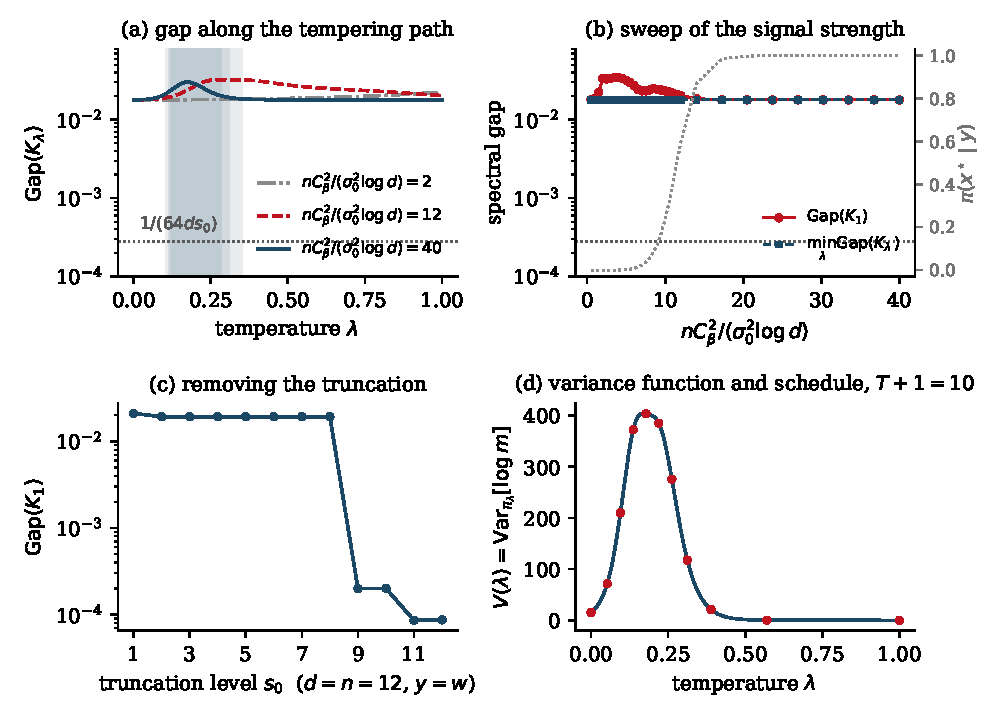
\includegraphics[width=\textwidth]{binary_numerics.pdf}
        \caption{Exact computations on small instances.
        \textbf{(a)} $\Gap(K_\lambda)$ along the tempering
        path~\eqref{eq:binary_path} for three signal strengths; the shaded
        band is the union of the intervals of
        Proposition~\ref{prop:binary_badset} on which the margin
        condition~\eqref{eq:binary_margin} fails, for the strongest signal;
        the dotted line is the bound $1/(64ds_0)$ of
        Theorem~\ref{th:binary_gap_margin}.
        \textbf{(b)} $\Gap(K_1)$ and $\min_{\lambda\in[0,1]}\Gap(K_\lambda)$
        as the signal strength sweeps through the range in which the posterior
        mass $\pi(x^{\star}\mid y)$ (dotted, right axis) moves from $0$ to $1$.
        \textbf{(c)} $\Gap(K_1)$ as a function of the truncation level $s_0$
        for the example of \citet[Appendix~B]{YangWainwrightJordan2016}:
        $d=n=12$ and $y=w$ pure noise.
        \textbf{(d)} the variance function $V$ of~\eqref{eq:binary_V} and the
        schedule~\eqref{eq:binary_schedule} it produces (dots).}
        \label{fig:binary_numerics}
    \end{figure}

    \paragraph{(a) The gap along the path}
    Over the whole sweep and the whole path, $\Gap(K_\lambda)$ stays in
    $[1.79\times10^{-2},\,3.45\times10^{-2}]$: it varies by less than a factor
    two, in $\lambda$ and in the signal strength together. The bound
    $1/(64ds_0)=2.79\times10^{-4}$ of Theorem~\ref{th:binary_gap_margin} holds,
    with a slack between $64$ and $124$. The slack is accounted for by the two
    crude steps of that proof: at $\lambda=0$ the measured gap is
    $1.7948\times10^{-2}$, against $1/(4d)=1.7857\times10^{-2}$, so the chain
    essentially realises the single-flip proposal probability of
    Lemma~\ref{lemma:binary_edge}, and what the bound gives away is the
    congestion factor $\Cong\leq16d$ and the length factor
    $\Len\leq4s_0$ of Theorem~\ref{th:binary_gap_margin}, whose product is
    $64s_0$.

    The shaded band is where the margin condition~\eqref{eq:binary_margin}
    fails. For the strongest signal it is the union of the three intervals
    $(0.114,0.353)$, $(0.119,0.286)$, $(0.104,0.310)$, which
    Proposition~\ref{prop:binary_badset} predicts to be contained in $[0,1]$
    and to exclude both endpoints, and on part of which all three influential
    covariates fail simultaneously, so $k_\lambda=3$. With
    $\Spread=10.6$ there, the factor
    $(8s^{\star}e^{\Spread})^{k_\lambda+1}$ of
    Theorem~\ref{th:binary_gap_hybrid} exceeds $10^{30}$. The measured gap on
    that band is not smaller than elsewhere; it is slightly larger. On this
    instance the price paid by Theorem~\ref{th:binary_gap_hybrid} is therefore
    an artefact of the proof and not a feature of the chain. That is a
    statement about this instance only; we do not claim that
    $e^{\Spread}$ can be removed in general, and
    Remark~\ref{rem:binary_price} recalls why some such factor must remain.

    \paragraph{(b) Sweeping the signal strength}
    As $nC_\beta^{2}/(\sigma_0^{2}\log d)$ runs from $0.5$ to $40$, the
    posterior mass $\pi(x^{\star}\mid y)$ moves from $0$ to $0.998$, so the
    sweep does cross the range in which the model is neither clearly
    identified nor clearly unidentifiable. Neither $\Gap(K_1)$ nor
    $\min_{\lambda}\Gap(K_\lambda)$ moves by more than a factor two across the
    sweep, and both stay two orders of magnitude above the bound.

    Two caveats. First, $\min_\lambda\Gap(K_\lambda)$ is attained at
    $\lambda=0$ for most of the sweep, and $\pi_0=p$ does not depend on the
    data, so the flatness of that curve is in part by construction; the
    informative curve is $\Gap(K_1)$. Second, this is one design at one small
    dimension, and a gap that does not collapse here is not evidence that it
    cannot collapse. Panel~(c) exhibits an instance where $\Gap(K_1)$ does
    collapse. Nor does anything here compare SMC with MCMC: the cost of SMC
    involves the horizon $T$ and, for standard SMC, the overhead $\mathcal D$
    of Lemma~\ref{lemma:binary_taubeta}, none of which is a spectral gap.

    \paragraph{(c) Removing the truncation}
    \citet[Appendix~B]{YangWainwrightJordan2016} show that with $d=n$, with
    $y=w$ pure noise, and with the sparsity prior left untruncated, the
    saturated model becomes a trap: it has $R^{2}=1$, so its marginal
    likelihood is large, and every neighbour is exponentially lighter. Panel
    (c) reproduces this with $d=n=12$, $\kappa=2$, $\alpha=3/2$, sweeping the
    truncation level. For $s_0\leq8$ the gap is $1.92\times10^{-2}$,
    independent of $s_0$; at $s_0=9$ it drops to $2.0\times10^{-4}$ and at
    $s_0=d=12$ to $8.7\times10^{-5}$, a factor $221$. This is the concrete
    content of item~2 of Section~\ref{sub:binary_practice}: the constraint
    $\abs x\leq s_0$ in the prior~\eqref{eq:binary_prior} is not a technical
    convenience, and the uniform prior on $\{0,1\}^{d}$ used by
    \citet{Schafer2013-yq} sits on the wrong side of it.

    \paragraph{(d) The schedule}
    The variance function $V$ of~\eqref{eq:binary_V} is concentrated near
    $\lambda\approx0.2$, which is where the mass of $\pi_\lambda$ leaves the
    null model, and it is nearly zero on $[0.5,1]$. The
    schedule~\eqref{eq:binary_schedule} places its steps accordingly: ten
    steps in all, of which eight lie in $[0,0.4]$, the last one covering
    $[0.57,1]$. The crude bound~\eqref{eq:binary_T_crude} gives
    $\lceil\sqrt{\bar V/\log2}\rceil=25$, so it is loose by a factor $2.5$
    here, which is what one expects from a bound that pays the worst variance
    along the whole path.


    %% ==================================================================
    \subsection{From spectral gaps to $\beta$-mixing times}
    \label{sub:binary_taubeta}
    %% ==================================================================

    Theorems~\ref{th:main_thm}, \ref{th:normalising_smc}
    and~\ref{th:boosted_smc}, which govern standard SMC, are stated in terms of
    the $\beta$-mixing time $\tau_\beta$ rather than of the spectral gap.
    Section~\ref{sec:spectral_gap_limitation} showed that the two can be far
    apart in either direction. On a finite space they differ by at most
    $\tfrac12\log\abs{\ambientspace}$, and in the direction unfavourable to
    standard SMC.

    \begin{lemma}
        \label{lemma:binary_taubeta}
        Let $\ambientspace$ be finite and let $K$ be reversible and
        non-negative definite with respect to a probability measure
        $\pi_\bullet$ of full support, with spectral gap $\gamma_\bullet>0$.
        Then for all $\xi\in(0,1)$ and $\omega\geq1$,
        \begin{equation}
            \label{eq:binary_taubeta}
            \tau_\beta(\xi,\omega,K)\ \leq\
            \frac{1}{\gamma_\bullet}\left(\frac12\log\abs{\ambientspace}
            +\log\frac{\omega}{2\xi}\right).
        \end{equation}
    \end{lemma}

    \begin{proof}
        \emph{Step 1: from $\chi^{2}$ to total variation.} For any probability
        measure $\mu\ll\pi_\bullet$, Cauchy--Schwarz gives
        \begin{equation*}
            2\,\TV(\mu,\pi_\bullet)
            =\sum_{z}\pi_\bullet(z)
            \left|\frac{\mu(z)}{\pi_\bullet(z)}-1\right|
            \ \leq\ \left\{\sum_z\pi_\bullet(z)
            \left(\frac{\mu(z)}{\pi_\bullet(z)}-1\right)^{2}\right\}^{1/2}
            =\chi^{2}(\mu\mid\pi_\bullet)^{1/2} .
        \end{equation*}

        \emph{Step 2: contraction.} A $\pi_\bullet$-reversible, non-negative
        definite kernel with spectral gap $\gamma_\bullet$ has operator norm
        $1-\gamma_\bullet$ on $\calL^{2}_{0,\pi_\bullet}$; applying this to
        $h=\dd\mu/\dd\pi_\bullet-1$, whose $\calL^{2}$-norm squared is
        $\chi^{2}(\mu\mid\pi_\bullet)$, gives
        $\chi^{2}(\mu K\mid\pi_\bullet)\leq(1-\gamma_\bullet)^{2}
        \chi^{2}(\mu\mid\pi_\bullet)$ and, by iteration,
        \begin{equation*}
            \chi^{2}(\delta_xK^{q}\mid\pi_\bullet)
            \ \leq\ (1-\gamma_\bullet)^{2q}
            \chi^{2}(\delta_x\mid\pi_\bullet)
            =(1-\gamma_\bullet)^{2q}
            \left\{\frac{1}{\pi_\bullet(x)}-1\right\}.
        \end{equation*}
        With Step~1, $\TV(\delta_xK^{q},\pi_\bullet)\leq
        \tfrac12(1-\gamma_\bullet)^{q}\pi_\bullet(x)^{-1/2}$.

        \emph{Step 3: averaging over a warm start.} Let $\mu$ be
        $\omega$-warm, that is $\mu(x)\leq\omega\pi_\bullet(x)$ for every $x$.
        Then
        \begin{equation*}
            \int\TV(\delta_xK^{q},\pi_\bullet)\,\mu(\dd x)
            \ \leq\ \frac{\omega}{2}(1-\gamma_\bullet)^{q}
            \sum_{x\in\ambientspace}\pi_\bullet(x)\pi_\bullet(x)^{-1/2}
            =\frac{\omega}{2}(1-\gamma_\bullet)^{q}
            \sum_{x}\pi_\bullet(x)^{1/2}
            \ \leq\ \frac{\omega}{2}(1-\gamma_\bullet)^{q}
            \abs{\ambientspace}^{1/2},
        \end{equation*}
        the last step by Cauchy--Schwarz,
        $\sum_x\pi_\bullet(x)^{1/2}\leq\{\abs{\ambientspace}
        \sum_x\pi_\bullet(x)\}^{1/2}$. Using $(1-\gamma_\bullet)^{q}\leq
        e^{-\gamma_\bullet q}$ and requiring the right-hand side to be at most
        $\xi$ gives~\eqref{eq:binary_taubeta}.
    \end{proof}

    Since
    $\abs{\ambientspace}=\sum_{k\leq s_0}\binom dk\leq(ed/s_0)^{s_0}$, the
    overhead of $\tau_\beta$ over $1/\gamma_\bullet$ is at most
    \begin{equation}
        \label{eq:binary_D}
        \mathcal{D}\ \coloneq\ \tfrac12\log\abs{\ambientspace}
        \ \leq\ \frac{s_0}{2}\log\frac{ed}{s_0} .
    \end{equation}
    It is a power of $s_0$, not a logarithm of it, and it is the price standard
    SMC pays over waste-free SMC on this problem. The contrast with the
    continuous case of Section~\ref{sec:spectral_gap_limitation} is
    instructive: there, a warm-start device
    (Proposition~\ref{prop:smc_mala_warm_start}) made $\tau_\beta$ smaller than
    $\gamma^{-1}$; here $\mathcal D$ comes from $\min_x\pi_\bullet(x)$ being
    exponentially small in $s_0$, and no analogue of that device is available.


    %% ==================================================================
    \subsection{Complexity}
    \label{sub:binary_complexity}
    %% ==================================================================

    We now collect the three inputs. Write
    \begin{equation}
        \label{eq:binary_G}
        \mathcal{G}\ \coloneq\ \min\Bigl\{
        1792\ d^{2}s_0s^{\star}2^{s^{\star}}d^{\kappa s^{\star}}
        e^{\Omega_\star},\ \
        7168\ d^{2}s_0\max(k_\star,1)
        \bigl(8s^{\star}e^{\Spread}\bigr)^{k_\star+1}\Bigr\},
        \qquad
        k_\star\coloneq\max_{t=0,\dots,T}k_{\lambda_t},
    \end{equation}
    for the inverse spectral gap, the better of
    Theorems~\ref{th:binary_gap_all} and~\ref{th:binary_gap_hybrid} along the
    schedule; $\mathcal D$ as in~\eqref{eq:binary_D} for the mixing-time
    overhead of Lemma~\ref{lemma:binary_taubeta}; and
    $T\leq C_V\sqrt{\mathcal{J}_\star/\log2}$ for the horizon of
    Proposition~\ref{prop:binary_horizon}\ref{it:binary_horizon_kl} with
    Corollary~\ref{cor:binary_J}.

    \begin{theorem}
        \label{th:binary_main}
        Assume the hypotheses of Theorem~\ref{th:binary_gap_all} and of
        Corollary~\ref{cor:binary_J}, and run the samplers of
        \cref{alg:smc,alg:wf_smc,alg:smc_size,alg:boosted} on the
        path~\eqref{eq:binary_path} with the schedule~\eqref{eq:binary_schedule}
        and the kernels $K_{\lambda_t}$. Then, on the event $\Good$,
        Assumptions~\ref{ass:chisquare_is_small} and~\ref{ass:spg} hold with
        $\gamma\geq1/\mathcal{G}$ as in~\eqref{eq:binary_G}, and the number of
        Markov steps sufficient for~\eqref{eq:garantee}, respectively
        for~\eqref{eq:garantee_Z}, is bounded as follows, up to factors
        logarithmic in $T$, $1/\eta$ and $1/\varepsilon$.
        \begin{center}
            \begin{tabular}{c|c|c}
                \arrayrulecolor{black}
                \textbf{Estimate} & \textbf{Algorithm} & \textbf{Markov steps} \\
                \hline
                \multirow{3}{*}{$\widehat\pi_{T-1}(f)$}
                & Alg.~\ref{alg:smc}
                & $T\,\mathcal{G}\,\mathcal{D}\,\varepsilon^{-2}$ \\
                \hhline{~--}
                & Alg.~\ref{alg:wf_smc}
                & \newres $T\,\mathcal{G}\,\varepsilon^{-2}$ \\
                \hhline{~--}
                & Alg.~\ref{alg:smc_size}
                & \newres $\mathcal{G}\,(T+\varepsilon^{-2})$ \\
                \hline
                \multirow{4}{*}{$\widehat Z_T$}
                & Alg.~\ref{alg:smc}
                & \newres $T^4\,\mathcal{G}\,\mathcal{D}\,\varepsilon^{-2}$ \\
                \hhline{~--}
                & Alg.~\ref{alg:smc} with medians
                & \newres $T^3\,\mathcal{G}\,\mathcal{D}\,\varepsilon^{-2}$ \\
                \hhline{~--}
                & Alg.~\ref{alg:wf_smc}
                & \newres $T^4\,\mathcal{G}\,\varepsilon^{-2}$ \\
                \hhline{~--}
                & Alg.~\ref{alg:boosted}
                & \newres $T^3\,\mathcal{G}\,\varepsilon^{-2}$ \\
                \hline
            \end{tabular}
        \end{center}
        The rows for $\widehat Z_T$ using Algorithms~\ref{alg:smc}
        and~\ref{alg:wf_smc} hold with $\eta=1/4$.
    \end{theorem}

    \begin{proof}
        Assumption~\ref{ass:chisquare_is_small} holds along the
        schedule~\eqref{eq:binary_schedule} by
        Proposition~\ref{prop:binary_horizon}\ref{it:binary_schedule}, and
        Assumption~\ref{ass:spg} holds with $\gamma\geq1/\mathcal G$ by
        Theorems~\ref{th:binary_gap_all} and~\ref{th:binary_gap_hybrid},
        applied at each $\lambda_t\in[0,1]$. Since $K_{\lambda_t}$ is
        non-negative definite, Lemma~\ref{lemma:binary_taubeta} applies and
        gives, for every $t$,
        \begin{equation}
            \label{eq:binary_taubeta_G}
            \tau_\beta(\xi,2,K_{\lambda_t})\ \leq\
            \mathcal{G}\bigl\{\mathcal{D}+\log(1/\xi)\bigr\},
        \end{equation}
        using $\log(2/(2\xi))=\log(1/\xi)$; hence the same bound for the
        uniform $\tau_\beta(\xi,2)$ of Section~\ref{sec:smc}. The total number
        of Markov steps is $(T+1)MP$ for Algorithms~\ref{alg:smc}
        and~\ref{alg:wf_smc}, $M\sum_{t}P_t$ for Algorithm~\ref{alg:smc_size},
        and $J(T+1)MP$ for Algorithm~\ref{alg:boosted}. The seven rows follow.
        \begin{itemize}[leftmargin=1.6em]
            \item Row~1. Theorem~\ref{th:main_thm} with $\bar\chi^{2}=2$ needs
            $M=\OO(\varepsilon^{-2}\log(T/\eta))$ and
            $P\geq\tau_\beta(\eta/(2MT),2)
            =\OO(\mathcal G\{\mathcal D+\log(MT/\eta)\})$
            by~\eqref{eq:binary_taubeta_G}. Hence
            $(T+1)MP=\widetilde\OO(T\mathcal G\mathcal D\varepsilon^{-2})$.
            \item Rows~2 and~3. Theorems~\ref{th:main_wf}
            and~\ref{th:wf_smc_greedy} with $M=1$ and
            $\gamma^{-1}\leq\mathcal G$; for Row~3 the greedy schedule has
            $P_t=\OO(\mathcal G\log(T/\eta))$ for $t<T$ and
            $P_T=\OO(\mathcal G\varepsilon^{-2}\log(T/\eta))$, whose sum is
            $\widetilde\OO(\mathcal G(T+\varepsilon^{-2}))$.
            \item Row~4. Theorem~\ref{th:normalising_smc} with
            $M=\Omega(T^{3}\varepsilon^{-2})$ and
            $P=\Omega(\tau_\beta(1/(MT)))$.
            \item Row~5. Theorem~\ref{th:boosted_smc} with
            $J=\Omega(\log(T/\eta))$, $M=\Omega(T^{2}\varepsilon^{-2})$ and
            $P=\Omega(\tau_\beta(1/(MT)))$.
            \item Rows~6 and~7. Theorems~\ref{th:strong_normalising_constant}
            and~\ref{th:boosted} with $M=1$ and, respectively,
            $P=\Omega(T^{3}\gamma^{-1}\varepsilon^{-2})$ and
            $P=\Omega(T^{2}\gamma^{-1}\varepsilon^{-2})$ with
            $J=\Omega(\log(T/\eta))$. \qedhere
        \end{itemize}
    \end{proof}

    \begin{corollary}[The polynomial regime]
        \label{cor:binary_poly}
        Take $\kappa,\alpha,L,\Ltil,C_m,r,c_2,s^{\star},C_V,\Spread,k_\star
        =\OO(1)$ and a signal at the detection threshold in the sense of
        Remark~\ref{rem:binary_E}, so that $\Energy=\OO(\log d)$,
        $\Omega_\star=\mathcal{J}_\star=\OO(\log d)$,
        $\mathcal G=\OO(s_0d^{q})$ for a constant
        $q$, $\mathcal D=\OO(s_0\log d)$ and $T=\OO(\sqrt{\log d})$. Then the
        marginal likelihood is estimated within relative error $\varepsilon$
        with probability $1-\eta$ using
        \begin{equation*}
            \widetilde\OO\bigl(d^{q}s_0(\log d)^{3/2}\varepsilon^{-2}\bigr)
            \quad\text{Markov steps by Algorithm~\ref{alg:boosted}, that is}
            \quad
            \widetilde\OO\bigl(n\,d^{q}s_0^{2}(\log d)^{3/2}
            \varepsilon^{-2}\bigr)\quad\text{operations,}
        \end{equation*}
        and $\pi(f)$ is estimated within absolute error $\varepsilon$ using
        $\widetilde\OO(d^{q}s_0\{\sqrt{\log d}+\varepsilon^{-2}\})$ Markov
        steps by Algorithm~\ref{alg:smc_size}. Both are polynomial in
        $(d,n,s_0,\varepsilon^{-1})$.
    \end{corollary}

    \begin{proof}
        Substitute the stated orders into the table of
        Theorem~\ref{th:binary_main}, using $T^{3}=\OO((\log d)^{3/2})$ for
        Algorithm~\ref{alg:boosted} and $T=\OO(\sqrt{\log d})$ for
        Algorithm~\ref{alg:smc_size}. The conversion into operations
        multiplies by the $\OO(ns_0+s_0^{2})=\OO(ns_0)$ cost of one evaluation
        of $m$, valid since $s_0<n$.
    \end{proof}

    \paragraph{Comparison with MCMC.}
    Corollary~1 of \citet{YangWainwrightJordan2016} states that the chain $K_1$
    started at the worst state returns $x^{\star}$ after
    $\OO(\alpha nds_0^{2}\log d)$ steps. Consider instead starting it at $\nu$,
    which is the only practical option and the one SMC uses. By the
    contraction inequality of Step~2 in the proof of
    Lemma~\ref{lemma:binary_taubeta}, the number of steps needed for the law of
    the chain to be within $\xi$ of $\pi$ is of order
    $\gamma^{-1}\{\ell_\nu+\log(1/\xi)\}$ with
    $\ell_\nu\coloneq\log\chi^{2}(\nu\mid\pi)$, and estimating $\pi(f)$ to
    accuracy $\varepsilon$ costs $\OO(\gamma^{-1}\varepsilon^{-2})$ further
    steps. Now $\chi^{2}(\nu\mid\pi)=\bbE_\nu[\dd\nu/\dd\pi]$, so Jensen's
    inequality gives
    \begin{equation*}
        \ell_\nu\ \geq\ \bbE_\nu\Bigl[\log\frac{\dd\nu}{\dd\pi}\Bigr]
        =\KL(\nu\mid\pi)\ \geq\ \mathcal{J}-\KL(\pi\mid\nu).
    \end{equation*}
    So MCMC pays $\widetilde\OO(\mathcal G\{\ell_\nu+\varepsilon^{-2}\})$ where
    Algorithm~\ref{alg:smc_size} pays
    $\widetilde\OO(\mathcal G\{\sqrt{\mathcal J}+\varepsilon^{-2}\})$: the cost
    of reaching the target from the prior falls from an amount proportional to
    $\mathcal J$ to one proportional to $\sqrt{\mathcal J}$. This is the
    general phenomenon of Section~\ref{sec:main}, here made explicit. Moreover
    MCMC returns no estimate of $Z_T$ with a comparable guarantee, which is the
    reason \citet{Schafer2013-yq} use SMC on this problem in the first place.


    %% ==================================================================
    \subsection{Consequences for practice}
    \label{sub:binary_practice}
    %% ==================================================================

    \begin{enumerate}[leftmargin=2.2em]
        \item \emph{Start from the prior, and temper the marginal likelihood
        only.} This is the path~\eqref{eq:binary_path}. Property~\ref{P:penalty}
        is what makes Theorems~\ref{th:binary_gap_all}
        and~\ref{th:binary_gap_hybrid} hold at every temperature: the penalty
        $d^{-\kappa}$ charged for each null covariate is the same at every
        $\lambda$, so the $d$ ways of adding one are beaten uniformly in
        $\lambda$ as soon as $\kappa>1$
        (Lemma~\ref{lemma:binary_block_mass}). Tempering the whole posterior,
        $\pi_\lambda\propto(pm)^{\lambda}$, destroys this. The initial
        distribution is then sampled exactly by~\ref{P:exact}, and
        $\widehat Z_T$ estimates the marginal likelihood directly.

        \item \emph{Take $\kappa>1$ and truncate at $s_0=\OO(n/\log d)$.}
        \citet{Schafer2013-yq} take the uniform prior on $\{0,1\}^{d}$, that is
        $\kappa=0$ and $s_0=d$. Then the $\lambda=0$ half of the sparsity
        budget~\eqref{eq:binary_budget_endpoints} fails,
        Lemma~\ref{lemma:binary_block_mass} fails with it, and so does every
        bound of Sections~\ref{sub:binary_gap} and~\ref{sub:binary_adapted};
        Assumption~\ref{ass:binary_D} fails as well. Both are repaired by the
        prior~\eqref{eq:binary_prior} with $\kappa>1$ and $s_0$ of the order
        that Assumption~\ref{ass:binary_D} allows. This is not only a
        limitation of the proof: panel~(c) of
        Figure~\ref{fig:binary_numerics} shows the exact gap of the local
        kernel dropping by a factor $221$ when the truncation is removed, on
        the example of \citet[Appendix~B]{YangWainwrightJordan2016}.

        \item \emph{Spend the sparsity budget: take
        $\kappa+\alpha\geq1+a_0+c_\kappa$.} This is
        Assumption~\ref{ass:binary_budget} at $\lambda=1$, in the form
        \eqref{eq:binary_budget_endpoints}: the sparsity penalty $d^{-\kappa}$
        and the Occam factor $(1+g)^{-\abs x/2}=d^{-\alpha+\OO(1)}$ must
        together beat both the $d$ ways of adding a covariate and the largest
        amount of likelihood $d^{a_0}$ that a null covariate can buy. By
        Propositions~\ref{prop:binary_null_over}
        and~\ref{prop:binary_null_gen}, $\kappa+\alpha\gtrsim L+\Ltil$ suffices
        when the proxy energy $\Xi$ of~\eqref{eq:binary_proxy} is $\OO(\log
        d)$, and $\kappa+\alpha=\Omega(s^{\star})$ is needed in the worst case.
        Since Assumption~\ref{ass:binary_C} constrains only $\kappa+\alpha$
        from below as well, and since $\kappa$ is also constrained on its own
        by the $\lambda=0$ half of~\eqref{eq:binary_budget_endpoints}, the
        practical recipe is: fix $\kappa$ slightly above $1$ for the prior end
        of the path, and then raise $\alpha$, that is $g$, until the budget
        holds at $\lambda=1$. Raising $\alpha$ is free.

        \item \emph{The local kernel has a polynomial but large inverse gap.}
        Theorem~\ref{th:binary_gap_all} gives $\gamma^{-1}\leq\mathcal G$,
        which without the margin condition is $d^{2+\kappa s^{\star}}$ up to
        factors. This is polynomial, and it is also large enough to explain the
        observation of \citet{Schafer2013-yq} that their sampler does not work
        with local kernels. Their global kernel, an independent
        Metropolis--Hastings kernel with a fitted proposal, has spectral gap
        equal to $\min_x q_{\theta_t}(x)/\pi_{t-1}(x)$, for which we have no
        lower bound and which can be exponentially small in $d$; we prove
        nothing about it.

        \item \emph{The exchange move is not needed.} The ensemble of
        Definition~\ref{def:binary_ensemble} uses single flips only, because it
        deletes null covariates before it adjusts the influential ones. So
        Theorems~\ref{th:binary_gap_margin} and~\ref{th:binary_gap_hybrid}, and
        also Proposition~\ref{prop:binary_within}, hold for the flip-only
        kernel, which is cheaper per step and simpler to implement than
        $K_\lambda$. As explained in Remark~\ref{rem:binary_beats}, the
        exchange move is what costs \citet{YangWainwrightJordan2016} the second
        factor $s_0$ in their $\OO(1/(ds_0^{2}))$.

        \item \emph{Use Algorithm~\ref{alg:smc_size} for moments and
        Algorithm~\ref{alg:boosted} for the marginal likelihood.} This is the
        recommendation of Section~\ref{sub:practical}, and it is reinforced
        here: standard SMC has no compensating advantage on this problem,
        because the factor $\mathcal{D}=\OO(s_0\log d)$ of
        Lemma~\ref{lemma:binary_taubeta} comes from $\min_x\pi_\bullet(x)$
        being exponentially small in $s_0$ and no analogue of
        Proposition~\ref{prop:smc_mala_warm_start} removes it.
    \end{enumerate}


    \bibliographystyle{imsart-nameyear}
    \bibliography{draft,bvs}

\end{document}
